\documentclass[11pt,a4paper]{article}

\usepackage[utf8]{inputenc}
\usepackage[T1]{fontenc}
\usepackage{lmodern}
\usepackage[margin=1.0in]{geometry}
\usepackage{amsmath,amssymb,amsfonts,amsthm}
\usepackage{booktabs}
\usepackage{graphicx}
\usepackage{xcolor}
\usepackage{hyperref}
\usepackage{float}
\usepackage{caption}
\usepackage{natbib}

\definecolor{darkblue}{RGB}{15,55,115}

\hypersetup{
    colorlinks=true,
    linkcolor=darkblue,
    citecolor=darkblue,
    urlcolor=darkblue,
    pdftitle={Seeing the Forest for the Polytomies: Minimum Description Length Phylogenetic Graph Induction Without Parametric Model Selection or Bootstrap Thresholds},
    pdfauthor={Sergei L. Kosakovsky Pond, Darren P. Martin, Stephanie J. Kosakovsky Pond, and Anton Nekrutenko}
}

\newtheorem{theorem}{Theorem}
\newtheorem{proposition}{Proposition}

\title{Seeing the Forest for the Polytomies: Minimum Description Length Phylogenetic Graph Induction Without Parametric Model Selection or Bootstrap Thresholds}
\author{Sergei L. Kosakovsky Pond$^{1}$, Darren P. Martin$^{2}$,\\
Stephanie J. Kosakovsky Pond$^{3}$, and Anton Nekrutenko$^{4}$\\[0.5em] % Stephanie ORCID: 0000-0002-8288-2232
\small $^{1}$Institute for Genomics and Evolutionary Medicine, Department of Biology,\\
\small Temple University, Philadelphia, PA, USA\\
\small $^{2}$Institute of Infectious Disease and Molecular Medicine, Department of Integrative Biomedical Sciences,\\
\small University of Cape Town, Cape Town, South Africa\\
\small $^{3}$Bioinnovation and Genomic Sciences Division,\\
\small Translational Genomics Research Institute, Phoenix, AZ, USA\\
\small $^{4}$Department of Biochemistry and Molecular Biology,\\
\small The Pennsylvania State University, University Park, PA, USA}
\date{November 10, 2026}

\begin{document}
\sloppy
\emergencystretch=1.5em
\maketitle

\begin{abstract}
Reconstructing evolutionary histories from biological sequences underpins nearly every discipline in the life sciences, from real-time pathogen surveillance and biodiversity discovery to comparative genomics and molecular evolution. Standard phylogenetic workflows separate substitution model selection, binary tree search, and branch support estimation into distinct stages, because classical information criteria penalize continuous rate parameters without pricing the discrete tree topology itself. Because descent with modification is physically an information-transmission process in which descendants inherit ancestral sequences and record only sparse mutations, phylogenetic inference can be recast as exact lossless data compression over both nucleotide and protein alphabets. We introduce Bushwhacker, an information-theoretic engine that evaluates evolutionary trees and networks under Rissanen's minimum description length principle across 4-state nucleotide and 20-state amino-acid alignments. Under this framework, every candidate branch must pay for its structural description by shortening the total code required to transmit the alignment. Polytomies emerge naturally whenever a split costs more information to specify than the mutations it explains, while horizontal gene transfers, recombination events, and convergent adaptations are captured whenever a lateral connection compresses the alignment further than a strict tree. Across 72,917 unique empirical alignments (93,495 nucleotide and protein runs) spanning the tree of life---including 7,200 model-selection alignments, all 45,205 eukaryotic phylogenomic loci across 19 datasets, 534 prokaryotic domain-wide and clinical \textit{Klebsiella} pangenome markers, pandemic viral cohorts of 10,062 SARS-CoV-2 and 5,498 dengue genomes, Poaceae $\text{C}_4$ photosynthetic horizontal transfers, and all 19,952 human-referenced mammalian genes and proteins across 882 species---and 22 simulation regimes, Bushwhacker collapses 96.4\% of model-dependent splits and 94.5\% of seed-unstable maximum-likelihood branches into polytomies, eliminates 61.5\% to 72.7\% of apparent eukaryotic and mammalian protein gene-tree conflict to resolve contentious animal, vertebrate, and placental origins, quantifies the archaeal Complexity Hypothesis in exact nats (20.6\% operational versus 0.0\% informational marker transfer), compresses pandemic SARS-CoV-2 cohorts to 63 bytes per genome (12.0$\times$ smaller than \texttt{gzip -9}), and resolves the mammalian convergence debate by confirming genome-wide bat--whale neutrality while isolating cochlear mechanotransduction convergence and a 25.8$\times$ excess in myrmecophagous pangolins and anteaters. Operating in milliseconds to seconds in a web browser or command line without substitution model sweeps or bootstrap resampling, Bushwhacker unifies model selection, polytomy resolution, and network inference through lossless evolutionary compression.
\end{abstract}

% ============================================================================
\section{Introduction}
% ============================================================================

Reconstructing evolutionary trees from molecular sequences is foundational to modern biology, providing the historical framework needed to track emerging epidemics, classify biodiversity across the tree of life, and trace the origins of genes, biochemical pathways, and complex traits \citep{felsenstein1981evolutionary,woese2000aminoacyl,parks2018gtdb}. In contemporary practice, parametric phylogenetic inference proceeds through three separate stages \citep{posada2004model}. First, an automated model selector such as ModelFinder evaluates candidate continuous-time Markov nucleotide or codon substitution matrices using the Akaike Information Criterion (AIC) or Bayesian Information Criterion (BIC) \citep{akaike1974new,schwarz1978estimating,kalyaanamoorthy2017modelfinder}. Second, a heuristic search engine explores the space of strictly bifurcating topologies to maximize the point log-likelihood $\ln P(A \mid T, \hat{\theta})$ under the selected rate matrix \citep{guindon2010new,price2010fasttree,kozlov2019raxml,minh2020iqtree}. Because this search always returns a fully resolved binary tree with $N - 3$ internal splits over $N$ taxa even when portions of the alignment lack mutational signal, practitioners append a third stage of post-hoc branch support evaluation using local likelihood-ratio tests \citep{anisimova2011survey} or bootstrap resampling \citep{felsenstein1985confidence,hoang2018ufboot2} to collapse weakly supported branches into polytomies \citep{zhang2018astral}.

As George Box observed fifty years ago, because all statistical models are approximations of reality, the scientist must remain alert to which aspects of a phenomenon a model captures and which it omits \citep{box1976science}. In standard phylogenetic model selection, classical information criteria measure model complexity solely through the continuous parameters of the substitution process. When evaluating a candidate substitution matrix on an alignment $A$ of $N$ taxa and $L$ columns, BIC computes $-2\ln P(A \mid T, \hat{\theta}) + k\ln L$ \citep{schwarz1978estimating}. In practice, phylogenetic software restricts the dimensional penalty $k\ln L$ to the $1$ to $10$ continuous exchangeability, stationary base-frequency, and rate-heterogeneity parameters of the $4 \times 4$ instantaneous rate matrix $Q$, while treating the discrete tree topology $T$ as unpenalized \citep{susko2020use}. Yet whereas the substitution matrix adjusts a handful of global continuous weights, an unrooted binary tree over $N$ taxa introduces $N - 3$ discrete bipartition choices selected from $(2N - 5)!!$ candidate topologies alongside $2N - 3$ continuous branch lengths. Optimizing a discrete binary topology across hundreds of taxa without charging a structural complexity cost for each resolved split inevitably resolves branches even when the expected number of substitutions along an internal edge falls below one.

Accounting for this unpenalized topological dimension clarifies recent debates over substitution model selection. Analyzing thousands of empirical and simulated nucleotide alignments, \citet{abadi2019model} reported that bypassing model selection altogether and fixing a parameter-rich general time-reversible matrix ($\text{GTR}+\text{I}+\text{G4}$) yields binary tree topologies nearly indistinguishable from those inferred under BIC-selected models. Re-examining the same empirical archive, \citet{gerth2019cannot} demonstrated that on alignments with low information content, $\text{GTR}+\text{I}+\text{G4}$ and BIC-selected models frequently recover conflicting binary trees, consistent with earlier findings by \citet{ripplinger2008does} and \citet{spielman2020relative}. Because both studies compared strictly bifurcating trees, neither asked whether the branches that differ between Jukes-Cantor, BIC, and $\text{GTR}+\text{I}+\text{G4}$ carry any mutational evidence. When an internal branch has an expected mutation load $\ell_e L < 1$, Poisson sampling frequently leaves zero substitutions on that edge in the observed alignment. On a zero-mutation branch, four-taxon likelihood differences vanish to first order, so small shifts in stationary base frequencies or transition-to-transversion weights alter the fourth-order numerical curvature among the three quartet resolutions and flip the resulting binary split.

Rissanen's Minimum Description Length (MDL) principle provides the exact, non-asymptotic foundation needed to price both continuous parameters and discrete graph structure in a single currency \citep{rissanen1978modeling,rissanen1983universal}. Classical BIC was derived by \citet{schwarz1978estimating} as an asymptotic Laplace approximation for smooth, interior continuous parameters in the large-sample limit $L \to \infty$, an expansion that breaks down on the boundary of tree space where branch lengths approach zero ($\ell_e = 0$) and does not price discrete bipartitions. Physically, biological replication along an evolutionary history is a causal delta-compression process in which each descendant lineage inherits its parental sequence and records only the sparse sites where mutations occurred. Under two-part MDL, an evolutionary hypothesis $\mathcal{G}$ and the alignment $A$ encoded conditional on $\mathcal{G}$ are measured in the same physical unit: natural logarithmic information units (nats). An unresolved star tree $T_{\text{star}}$ defines the universal zero-split null code length $\mathcal{L}_{\text{MDL}}(A, T_{\text{star}})$, and every candidate internal split $e$ must pay for its discrete bipartition address and mutated-site subset index out of the parsimony and branch-length savings it generates across the alignment.

Pricing evolutionary structure in nats unifies substitution modeling, polytomy resolution, and reticulate network inference within a single objective. Under MDL, multifurcating polytomies emerge naturally during tree induction without bootstrap resampling or user-defined support cutoffs: any internal split whose description-length savings do not exceed its structural header ($G_{\text{MDL}}(e) \le 0\text{ nats}$, the exact information-theoretic break-even threshold where adding the split lengthens the total code) is contracted into a multifurcating hub. By the same principle, MDL extends directly from trees to reticulate evolutionary graphs. Whereas adding a horizontal gene transfer tract or a convergent amino-acid substitution edge to a tree always increases the in-sample log-likelihood, MDL certifies a lateral shunt between non-sister lineages only when the vertical mutation costs it eliminates exceed the exact address cost of specifying the donor branch, recipient branch, and affected site mask. Here we introduce Bushwhacker (\textbf{B}ipartition \textbf{U}nification, \textbf{S}hunt \textbf{H}unting, and \textbf{W}eighted \textbf{H}ub \textbf{A}ggregation via \textbf{C}ombinadic \textbf{K}olmogorov \textbf{E}ntropy \textbf{R}eduction), an information-theoretic phylogenetic graph induction engine and lossless compressor (\texttt{.bwz}) over 4-state nucleotide and 20-state amino-acid alphabets written in bit-parallel Rust and WebAssembly. We first derive the two-part MDL objective for nucleotide and protein alignments and illustrate its behavior on a four-taxon worked example. We then evaluate Bushwhacker across a 22-scenario suite of simulated alignment datasets created with AliSim \citep{lytrong2022alisim} and 72,917 empirical alignments (93,495 total nucleotide and amino-acid runs): all 7,200 alignments from \citet{abadi2019model} and \citet{gerth2019cannot}, all 19 eukaryotic phylogenomic datasets (45,205 single-gene DNA and protein alignments) from \citet{zhou2018evaluating}, 534 prokaryotic domain-wide and clinical pangenome alignments from the Genome Taxonomy Database \citep{parks2018gtdb,parks2020gtdb} and the \textit{Klebsiella pneumoniae} complex \citep{wyres2020population}, all 19,952 human-referenced mammalian coding genes and translated proteins across 882 genome assemblies from TOGA2 \citep{kirilenko2023integrating,malovichko2026toga2}, Poaceae $\text{C}_4$ photosynthetic lateral gene transfer datasets \citep{christin2007c4,christin2012adaptive}, and pandemic-scale SARS-CoV-2, global dengue (\texttt{DENV-1..4}), and HIV-1 recombinant genome cohorts.

% ============================================================================
\section{Mathematical Formulation: Two-Part MDL Graph Induction}
% ============================================================================

\subsection{The Star-Tree Null Baseline and Phylogenetic Compressibility}

In maximum-likelihood phylogenetics, a substitution model and tree $T$ assign a joint probability $P(A \mid T)$ to a multiple sequence alignment $A$, and the negative log-likelihood $-\ln P(A \mid T)$ is mathematically identical to the number of natural logarithmic information units (nats, where $1\text{ nat} = 1/\ln 2 \approx 1.44\text{ bits}$) required to encode the alignment conditional on $T$. Two-part Minimum Description Length (MDL) extends this likelihood principle by pricing both the evolutionary graph $\mathcal{G}$ and the alignment encoded along $\mathcal{G}$ on the same scale: $\mathcal{L}_{\text{MDL}}(A, \mathcal{G}) = \mathcal{L}(\mathcal{G}) + \mathcal{L}(A \mid \mathcal{G})$ \citep{rissanen1978modeling,rissanen1983universal}. To measure how much hierarchical evolutionary structure an alignment contains, we first establish the baseline cost of encoding the sequences on an unresolved star phylogeny $T_{\text{star}}$ with zero internal branches ($|E_{\text{int}}| = 0$). Let $A \in \Sigma^{N \times L}$ denote an alignment over $N$ taxa and $L$ columns on the nucleotide alphabet $\Sigma = \{\text{A, C, G, T}\}$. Recording the raw alignment without any shared ancestry requires $N L_{\text{eff}} \ln 4$ nats across the $L_{\text{eff}}$ ungapped cells ($\ln 4 \approx 1.39\text{ nats}$, or $2\text{ bits}$, per nucleotide). Under the star phylogeny $T_{\text{star}}$, all $N$ taxa diverge independently from a single ancestral root sequence $X_r$. Recording $X_r$ once costs $L \ln 4$ nats, after which each terminal branch $i \in \{1, \dots, N\}$ inherits $X_r$ and records only the $m_i$ autapomorphic sites (lineage-specific mutations unique to a single terminal taxon) where taxon $i$ differs from the root across its $L_{\text{eff}, i}$ ungapped columns:
\begin{equation}
    \mathcal{L}_{\text{branch}}(m_i, L_{\text{eff}, i}) \;=\; \ln 2 + \mathcal{L}_{\mathbb{N}}(m_i) + \ln\binom{L_{\text{eff}, i}}{m_i} + \sum_{k=1}^{m_i} \ell_{\text{subst}}(a_{i,k} \to b_{i,k}).
    \label{eq:branch_code}
\end{equation}
Each of the four terms in Equation~\eqref{eq:branch_code} has a direct phylogenetic interpretation. The leading $\ln 2$ ($1\text{ bit}$) records whether branch $i$ carries at least one substitution ($m_i > 0$) versus zero substitutions ($m_i = 0$), while $\mathcal{L}_{\mathbb{N}}(m_i) = \ln(1 + m_i) + \frac{1}{2}\ln(1 + \ln(1 + m_i))$ is Rissanen's universal integer complexity penalty for recording the discrete branch length $m_i$ when the mutation count is unknown in advance \citep{rissanen1983universal}. Next, $\ln\binom{L_{\text{eff}, i}}{m_i}$ is the combinadic site-subset index specifying which $m_i$ alignment columns mutated along branch $i$, and $\ell_{\text{subst}}(a_{i,k} \to b_{i,k}) = -\ln P(b_{i,k} \mid a_{i,k})$ is the negative log-probability of substituting ancestral base $a_{i,k}$ with derived base $b_{i,k}$ ($\ln 3 \approx 1.10\text{ nats}$ under equal substitution rates). The combinadic site-subset term $\ln\binom{L_{\text{eff}, i}}{m_i}$ is essential to this formulation for three evolutionary and statistical reasons. First, because substitutions at different sites along a branch have no intrinsic arrival order across alignment columns, listing $m_i$ site coordinates one by one would cost $m_i\ln L_{\text{eff}, i}$ nats and waste $\ln(m_i!)$ nats specifying an arbitrary column ordering. Indexing the unordered subset of $m_i$ mutated sites among all $\binom{L_{\text{eff}, i}}{m_i}$ possible site combinations eliminates this $\ln(m_i!)$ redundancy. Second, dividing out $m_i!$ makes the positional cost sub-additive as $m_i$ grows, so multiple synapomorphies (shared derived mutations inherited from a common ancestor) mapped to the same internal branch pool their overhead while rapidly evolving branches receive a lower per-site weight than slowly evolving branches. Third, conditioned on $m_i$ substitutions occurring along branch $i$, all $\binom{L_{\text{eff}, i}}{m_i}$ site subsets have equal probability $1/\binom{L_{\text{eff}, i}}{m_i}$ (matching the exact marginal likelihood after integrating out the unknown continuous branch length), which vanishes on zero-mutation branches ($m_i = 0$, $\ln\binom{L_{\text{eff}, i}}{0} = 0$) where asymptotic BIC penalties break down.

Summing Equation~\eqref{eq:branch_code} across the ancestral root sequence and all $N$ terminal branches yields the star-tree null description length $\mathcal{L}_{\text{MDL}}(A, T_{\text{star}})$, which serves as the universal zero-split baseline for any candidate evolutionary graph $\mathcal{G}^* = (V, E_{\text{tree}}, E_{\text{shunt}})$. On the star tree, any synapomorphy shared by a clade of descendant taxa must be recorded repeatedly as homoplasies (independent parallel or convergent mutations to the same state on separate lineages) on each descendant leaf. Adding an internal branch or lateral shunt to $T_{\text{star}}$ shortens those descendant branch descriptions by factoring shared derived mutations onto a single ancestral edge, at the price of adding the new branch's own mutation record and topological split address. Comparing the total description length of the inferred graph $\mathcal{G}^*$ against the star tree defines the Phylogenetic Compression Ratio:
\begin{equation}
    \rho(A) \;=\; 1 - \frac{\mathcal{L}_{\text{MDL}}(A, \mathcal{G}^*)}{\mathcal{L}_{\text{MDL}}(A, T_{\text{star}})}.
    \label{eq:comp_ratio}
\end{equation}
Equation~\eqref{eq:comp_ratio} provides a bounded, dimensionless measure of hierarchical phylogenetic signal that requires no parametric substitution model sweep or bootstrap resampling. Alignments evolved on a true star radiation or scrambled by complete mutational saturation yield $\rho(A) = 0$, because no internal split eliminates enough parallel leaf mutations to pay for its own structural cost. Conversely, alignments with well-supported clade stems and moderate terminal divergence achieve high values of $\rho(A)$, as single synapomorphies recorded on deep internal branches eliminate dozens of duplicate entries across descendant leaves.

\subsection{Exact Bipartition Cost and the Natural Polytomy Law}

In phylogenetic terms, resolving a multifurcating polytomy node $w$ of degree $d = k_u + k_v \ge 4$ by inserting an internal branch $e = (u,v)$ divides its $d$ attached lineages into $k_u \ge 2$ lineages on side $u$ and $k_v \ge 2$ lineages on side $v$. Before recording any synapomorphies along $e$, the model must pay the topological complexity cost of specifying which bipartition of the $d$ lineages was selected out of all possible splits at node $w$. Without loss of generality, let $2 \le k_u \le k_v$. The model first specifies the unordered clade-size pair $\{k_u, k_v\}$ among the $\max(1, \lfloor d/2\rfloor - 1)$ non-trivial split sizes and then indexes the chosen subset of $k_u$ lineages. Dividing by $2$ when $k_u = k_v$ (because swapping equal-sized halves defines the same unrooted split) yields the topological split cost
\begin{equation}
    \mathcal{L}_{\text{topo}}(k_u, k_v) \;=\; \ln\,\max\!\left(1,\; \left\lfloor\frac{k_u + k_v}{2}\right\rfloor - 1\right) \;+\; \ln\binom{k_u + k_v}{k_u} \;-\; \mathbb{I}(k_u = k_v)\ln 2 \quad \text{nats}.
    \label{eq:topo_cost}
\end{equation}
When resolving a four-taxon polytomy into a bifurcating quartet ($k_u = 2, k_v = 2$), Equation~\eqref{eq:topo_cost} charges $\ln 1 + \ln\binom{4}{2} - \ln 2 = \ln 3 \approx 1.10$ nats, the exact information cost of selecting one of the three possible unrooted four-taxon tree topologies. At a five-lineage node ($k_u = 2, k_v = 3$), Equation~\eqref{eq:topo_cost} charges $\ln\binom{5}{2} = \ln 10 \approx 2.30$ nats. More generally, resolving a two-taxon sister pair ($k_u = 2$) out of a large polytomy radiation of degree $d \gg 4$ requires $\mathcal{L}_{\text{topo}}(2, d-2) = \ln(\lfloor d/2\rfloor - 1) + \ln\binom{d}{2} \approx 3\ln d - 2\ln 2$ nats, which acts as an automatic multiple-testing correction across all $\binom{d}{2}$ candidate sister-pairings at the radiation hub. Once this topological split cost $\mathcal{L}_{\text{topo}}(k_u, k_v)$ is paid, the candidate internal branch $e = (u,v)$ reduces the alignment description length by transferring shared derived mutations (synapomorphies) off its adjacent descendant branches and onto $e$. When $m_{e,c}$ substitutions on an adjacent branch $c$ (which carries $m_c$ total mutations) are transferred onto $e$, branch $c$'s description length drops by $\Delta\mathcal{L}_{\text{branch}}(c) = \mathcal{L}_{\text{branch}}(m_c, L_{\text{eff},c}) - \mathcal{L}_{\text{branch}}(m_c - m_{e,c}, L_{\text{eff},c})$. For a single transferred substitution, the binomial identity $\ln\binom{L_{\text{eff}}}{m_c + 1} - \ln\binom{L_{\text{eff}}}{m_c} = \ln\frac{L_{\text{eff}} - m_c}{m_c + 1}$ shows that removing one mutation from branch $c$ saves the marginal positional weight
\begin{equation}
    w_c \;=\; \ln\!\left(\frac{L_{\text{eff}} - m_c}{m_c + 1}\right) \quad \text{nats}.
    \label{eq:marginal_weight}
\end{equation}
In evolutionary terms, $w_c \approx -\ln\frac{p_c}{1 - p_c}$ (where $p_c = m_c / L_{\text{eff}}$ is the empirical substitution probability on branch $c$) matches the log-odds character weight derived by \citet{felsenstein1981evolutionary} for maximum likelihood under unequal branch lengths. Consequently, a synapomorphy shared between two slowly evolving lineages ($m_c \ll L_{\text{eff}}$, large $w_c$) provides much stronger evidence for common ancestry than a convergent state shared between two rapidly evolving lineages ($m_c$ large, small $w_c$). Each transferred synapomorphy also saves its nucleotide substitution cost $\ell_{\text{subst}}(a \to b)$ plus the incremental branch-length integer penalty $\mathcal{L}_{\mathbb{N}}(m_c + 1) - \mathcal{L}_{\mathbb{N}}(m_c)$. Let $\Delta\mathcal{L}_{\text{children}}(m)$ denote the total description-length reduction across the adjacent descendant branches when the top $m$ synapomorphic sites ($1 \le m \le K$) where split $e = (u,v)$ reduces Fitch parsimony steps \citep{fitch1971toward} or shifts substitutions from short branches onto long branches are transferred onto $e$. Resolving internal branch $e$ is supported if and only if its net MDL compression gain is strictly positive:
\begin{equation}
    G_{\text{MDL}}(e) \;\equiv\; -\Delta\mathcal{L}_{\text{MDL}}(e) \;=\; \max_{1 \le m \le K} \Big[ \Delta\mathcal{L}_{\text{children}}(m) - \mathcal{L}_{\text{branch}}(m, L_{\text{eff}}) \Big] - \mathcal{L}_{\text{topo}}(k_u, k_v) \;>\; 0.
    \label{eq:mdl_gain}
\end{equation}
Because description length is a negative log-probability, $G_{\text{MDL}}(e)$ is the exact log-Bayes factor (log-posterior odds ratio) favoring the resolved split $e$ over an unresolved polytomy. Whenever $G_{\text{MDL}}(e) \le 0$, collapsing branch $e$ into a multifurcating polytomy yields a more probable, shorter description of the alignment, whereas positive gains convert directly into a Bayesian posterior branch support probability $P(e \in E_{\text{tree}} \mid A) = \big(1 + \exp(-G_{\text{MDL}}(e))\big)^{-1}$ without bootstrap resampling or Markov chain Monte Carlo integration.

\subsection{Didactic Example: Grounding MDL Graph Induction on Four Taxa Across Sixteen Sites}

To make every term of the two-part MDL ledger concrete before moving to genome-scale alignments, consider an ungapped alignment $A$ of $N = 4$ taxa ($\text{T}_1, \text{T}_2, \text{T}_3, \text{T}_4$) across $L = 16$ nucleotide columns with ancestral root sequence $X_r = \texttt{A}^{16}$ and uniform substitution state cost $\ell_{\text{subst}} = \ln 3 \approx 1.10\text{ nats}$ (Figure~\ref{fig:didactic_mdl}A and Table~\ref{tab:worked_example}). Without an evolutionary model, transmitting all $4 \times 16 = 64$ characters requires $64 \ln 4 = 88.72\text{ nats}$, whereas transmitting the ancestral root sequence $X_r$ once requires $16 \ln 4 = 22.18\text{ nats}$. Suppose each of the four taxa carries $m_c = 2$ private terminal mutations distributed across sites $4\text{--}11$ (\texttt{C} at sites $4\text{--}5$ in $\text{T}_1$, \texttt{T} at sites $6\text{--}7$ in $\text{T}_2$, \texttt{C} at sites $8\text{--}9$ in $\text{T}_3$, and \texttt{T} at sites $10\text{--}11$ in $\text{T}_4$), while sites $12\text{--}16$ are invariant across all four taxa. Meanwhile, sites $1\text{--}3$ carry $m_e \in \{1, 2, 3\}$ candidate synapomorphies uniting $\{\text{T}_1, \text{T}_2\}$ in derived state \texttt{G} against $\{\text{T}_3, \text{T}_4\}$ in ancestral state \texttt{A}.

Applying Equation~\eqref{eq:branch_code} to a 16-site alignment reveals why multiple mutations on the same branch amortize their structural overhead. Encoding $m = 1, 2,$ or $3$ substitutions along any branch of length $L_{\text{eff}} = 16$ costs $\mathcal{L}_{\text{branch}}(1, 16) = 0.69 + 0.96 + 2.77 + 1.10 = 5.52\text{ nats}$, $\mathcal{L}_{\text{branch}}(2, 16) = 0.69 + 1.47 + 4.79 + 2.20 = 9.15\text{ nats}$, and $\mathcal{L}_{\text{branch}}(3, 16) = 0.69 + 1.82 + 6.33 + 3.30 = 12.14\text{ nats}$ (with $\mathcal{L}_{\text{branch}}(4, 16) = 14.68\text{ nats}$ and $\mathcal{L}_{\text{branch}}(5, 16) = 16.87\text{ nats}$). Thus the per-mutation cost drops from $5.52\text{ nats}$ at $m = 1$ to $4.58\text{ nats}$ at $m = 2$ and $4.05\text{ nats}$ at $m = 3$ (Figure~\ref{fig:didactic_mdl}A). Two mathematical effects drive this sub-additive scaling: the active-branch flag ($\ln 2 = 0.69\text{ nats}$) and integer count $\mathcal{L}_{\mathbb{N}}(m)$ are paid only once per branch, and the combinadic index $\ln\binom{16}{m} = \ln(16! / (m!(16-m)!))$ divides out all $m!$ redundant permutation orderings of the mutated site indices. Because each leaf already carries $m_c = 2$ private mutations ($\mathcal{L}_{\text{branch}}(2, 16) = 9.15\text{ nats}$), appending a third mutation to an existing leaf increases its combinadic site address by $w_c = \ln\binom{16}{3} - \ln\binom{16}{2} = \ln(14/3) = 1.54\text{ nats}$ (Equation~\eqref{eq:marginal_weight}) and its total branch code by $\mathcal{L}_{\text{branch}}(3, 16) - \mathcal{L}_{\text{branch}}(2, 16) = 12.14 - 9.15 = 2.99\text{ nats}$. Under the unresolved star tree $T_{\text{star}}$ (Figure~\ref{fig:didactic_mdl}B), $m_e$ shared \texttt{A}$\to$\texttt{G} synapomorphies must be encoded twice in parallel on leaves $\text{T}_1$ and $\text{T}_2$, raising their leaf codes to $2\,\mathcal{L}_{\text{branch}}(2 + m_e, 16)$.

Inserting the candidate internal edge $e = (\{\text{T}_1, \text{T}_2\}, \{\text{T}_3, \text{T}_4\})$ eliminates those duplicate leaf entries at the price of the quartet bipartition header $\mathcal{L}_{\text{topo}}(2,2) = \ln 3 = 1.10\text{ nats}$ plus the new internal branch code $\mathcal{L}_{\text{branch}}(m_e, 16)$ (Figure~\ref{fig:didactic_mdl}C and Table~\ref{tab:worked_example}). When only a single synapomorphy ($m_e = 1$) supports the split, removing that mutation from leaves $\text{T}_1$ and $\text{T}_2$ saves $\Delta\mathcal{L}_{\text{children}}(1) = 2(12.14 - 9.15) = 5.98\text{ nats}$, whereas opening a new internal branch to carry one mutation costs $\mathcal{L}_{\text{branch}}(1, 16) + \mathcal{L}_{\text{topo}}(2,2) = 5.52 + 1.10 = 6.62\text{ nats}$. Even though resolving the split saves one Fitch parsimony step, opening a separate branch and paying the $\ln 3$ quartet topology header for a single isolated site ($6.62\text{ nats}$) is more expensive than encoding that site on the two existing leaf branches ($5.98\text{ nats}$). As a result, the exact two-part gain is negative ($G_{\text{MDL}}(e) = 64.75 - 65.39 = -0.64\text{ nats} < 0$), and the algorithm contracts the weakly supported edge into a star polytomy. Once $m_e = 2$ or $m_e = 3$ shared synapomorphies support $\{\text{T}_1, \text{T}_2\}$, however, they share the single branch header and amortize the combinadic site address through $\ln(m_e!)$. Consequently, leaf savings $\Delta\mathcal{L}_{\text{children}}(m_e)$ reach $+11.07\text{ nats}$ at $m_e = 2$ and $+15.45\text{ nats}$ at $m_e = 3$, so $G_{\text{MDL}}(e)$ turns positive at $m_e = 2$ ($69.84 - 69.01 = +0.83\text{ nats}$, $P_{\text{MDL}} = 0.696$) and climbs to $+2.22\text{ nats}$ at $m_e = 3$ ($74.22 - 72.01\text{ nats}$, $P_{\text{MDL}} = 0.902$).

The same 16-site example also demonstrates why combinadic MDL resists Long-Branch Attraction in the Felsenstein Zone \citep{felsenstein1978cases} and prices lateral shunts on a single scale (Figure~\ref{fig:didactic_mdl}D). Suppose non-sister leaves $\text{T}_1$ and $\text{T}_3$ are rapidly evolving branches that carry $m_{\text{long}} = 6$ private mutations each, whereas $\text{T}_2$ and $\text{T}_4$ are slowly evolving branches that carry only $m_{\text{short}} = 1$ private mutation each. By Equation~\eqref{eq:marginal_weight}, absorbing a shared state off a quiet short branch saves $w_{\text{short}} = \ln\frac{16 - 1}{1 + 1} = \ln(7.5) = 2.01\text{ nats}$ of positional address, whereas absorbing a chance collision off a noisy six-mutation branch saves only $w_{\text{long}} = \ln\frac{16 - 6}{6 + 1} = \ln(10/7) = 0.36\text{ nats}$. Consequently, falsely grouping the two long branches $\{\text{T}_1, \text{T}_3\}$ on a convergent homoplasy saves just $2 w_{\text{long}} = 0.71\text{ nats}$ of positional code, whereas grouping the quiet branches saves $2 w_{\text{short}} = 4.03\text{ nats}$, giving true homology a $5.6$-fold positional compression advantage over long-branch attraction. Moreover, once the vertical backbone $((\text{T}_1,\text{T}_2),(\text{T}_3,\text{T}_4))$ is established, any block of $m$ parallel replacements shared between non-sister lineages $\text{T}_1$ and $\text{T}_3$ is peeled onto a Stage 4 lateral shunt if and only if its vertical leaf savings exceed the endpoint header $2\ln|V|$ plus the site-mask code $\min(\mathcal{L}_{\text{mask}}^{\text{INTERVAL}}, \mathcal{L}_{\text{mask}}^{\text{SPARSE}})$.

\begin{figure}[t!]
\centering
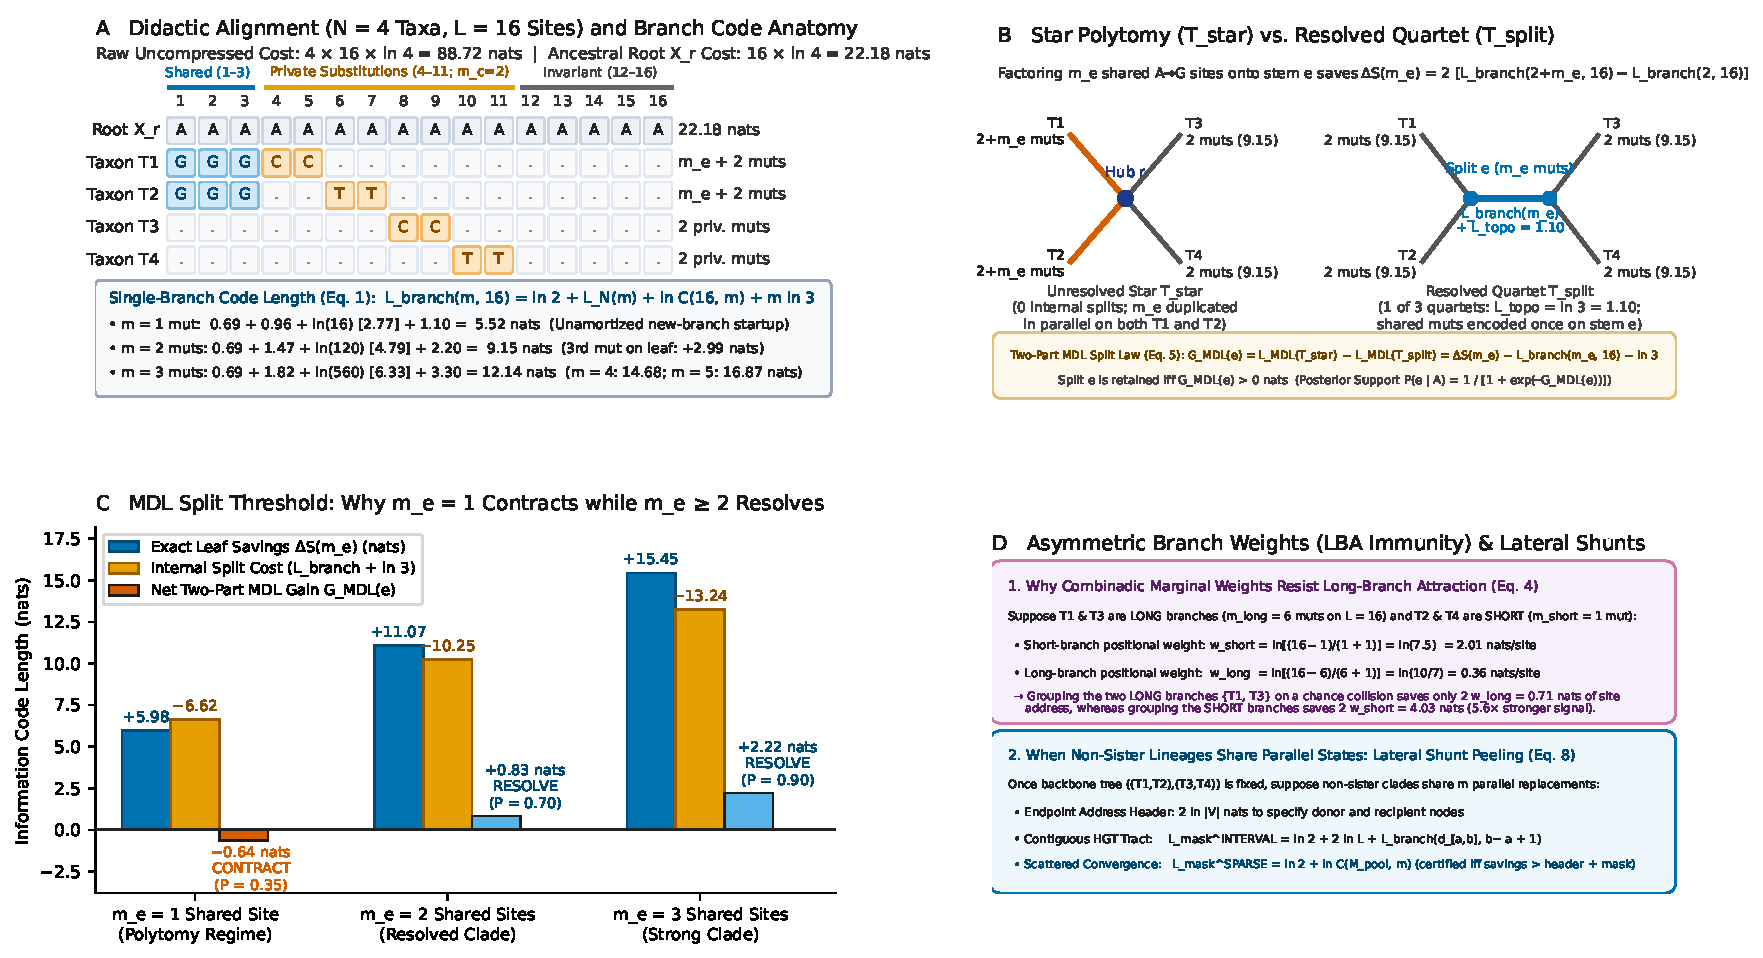
\includegraphics[width=\textwidth]{fig_didactic_mdl.pdf}
\caption{Two-part Minimum Description Length (MDL) graph induction prices discrete splits and reticulate shunts on a 4-taxon, 16-site alignment ($N = 4, L = 16$). Panel A shows the alignment matrix ($X_r = \texttt{A}^{16}$, with blue cells marking $m_e \in \{1,2,3\}$ shared \texttt{G} synapomorphies at sites $1\text{--}3$, orange cells marking $m_c = 2$ private leaf mutations at sites $4\text{--}11$, and gray dots marking invariant sites $12\text{--}16$) alongside single-branch code lengths $\mathcal{L}_{\text{branch}}(m, 16)$ from Equation~\eqref{eq:branch_code}. Panel B contrasts the unresolved star tree $T_{\text{star}}$ (vermillion parallel leaf edges) against the resolved quartet $T_{\text{split}}$ (blue internal stem $e$, $\mathcal{L}_{\text{topo}}(2,2) = \ln 3 = 1.10\text{ nats}$). Panel C plots exact leaf savings $\Delta\mathcal{L}_{\text{children}}(m_e)$ (blue bars), internal split cost $\mathcal{L}_{\text{branch}}(m_e,16) + \ln 3$ (orange bars), and net gain $G_{\text{MDL}}(e)$ across $m_e = 1, 2, 3$: a single synapomorphy ($m_e = 1$, vermillion negative bar, $G_{\text{MDL}} = -0.64\text{ nats}$) contracts into a polytomy, whereas $m_e \ge 2$ (sky-blue positive bars, $+0.83$ and $+2.22\text{ nats}$) amortizes the combinadic header and retains the split. Panel D summarizes combinadic marginal weight asymmetry ($w_{\text{short}} = 2.01\text{ nats}$ versus $w_{\text{long}} = 0.36\text{ nats}$) in the Felsenstein Zone and dual-mode lateral shunt pricing.}
\label{fig:didactic_mdl}
\end{figure}

\begin{table}[t!]
\centering
\caption{Worked MDL ledger for a 4-taxon, 16-site alignment ($N = 4, L = 16$, raw uncompressed cost $64\ln 4 = 88.72\text{ nats}$, root sequence cost $16\ln 4 = 22.18\text{ nats}$). Each taxon carries $m_c = 2$ private terminal mutations ($\mathcal{L}_{\text{branch}}(2, 16) = 9.15\text{ nats}$), while $m_e \in \{1, 2, 3\}$ shared synapomorphies at sites $1\text{--}3$ unite $\{\text{T}_1, \text{T}_2\}$ against $\{\text{T}_3, \text{T}_4\}$, so $G_{\text{MDL}}(e) \equiv \mathcal{L}_{\text{MDL}}(A, T_{\text{star}}) - \mathcal{L}_{\text{MDL}}(A, T_{\text{split}})$ holds identically.}
\label{tab:worked_example}
\footnotesize
\setlength{\tabcolsep}{4.5pt}
\resizebox{\textwidth}{!}{%
\begin{tabular}{@{}clccccccr@{}}
\toprule
Shared Sites & Alignment Pattern ($L = 16$ columns; dots match $\text{X}_r = \texttt{A}^{16}$) & Leaf Savings & Split Cost & Topo Cost & Exact Net Gain & Exact Two-Part & Posterior & Topology \\
$m_e$ & $\text{T}_1, \text{T}_2$ vs.\ $\text{T}_3, \text{T}_4$ (Sites $1\text{--}3 \mid 4\text{--}11 \mid 12\text{--}16$) & $\Delta\mathcal{L}_{\text{children}}(m_e)$ & $\mathcal{L}_{\text{branch}}(m_e, 16)$ & $\mathcal{L}_{\text{topo}}(2,2)$ & $G_{\text{MDL}}(e)$ & $T_{\text{star}} \to T_{\text{split}}$ & $P(e \mid A)$ & Decision \\
\midrule
$m_e = 1$ & $\text{T}_{1,2}: \texttt{G . .} \mid \text{2 priv.\ muts} \mid \texttt{. . . . .}$ & $+5.98$ & $-5.52$ & $-1.10$ & $-0.64\text{ nats}$ & $64.75 \to 65.39$ & $0.346$ & Contract ($T_{\text{star}}$) \\
$m_e = 2$ & $\text{T}_{1,2}: \texttt{G G .} \mid \text{2 priv.\ muts} \mid \texttt{. . . . .}$ & $+11.07$ & $-9.15$ & $-1.10$ & $+0.83\text{ nats}$ & $69.84 \to 69.01$ & $0.696$ & Resolve $(\text{T}_1,\text{T}_2)$ \\
$m_e = 3$ & $\text{T}_{1,2}: \texttt{G G G} \mid \text{2 priv.\ muts} \mid \texttt{. . . . .}$ & $+15.45$ & $-12.14$ & $-1.10$ & $+2.22\text{ nats}$ & $74.22 \to 72.01$ & $0.902$ & Resolve $(\text{T}_1,\text{T}_2)$ \\
\bottomrule
\end{tabular}%
}
\end{table}

\subsection{Algorithmic Workflow: Character-State Graph Induction Across Four Stages}

Having defined the two-part MDL scoring objective on individual branches and splits, we now describe how Bushwhacker constructs a calibrated multifurcating tree and reticulate network from an input multiple sequence alignment $A$ of $N$ taxa and $L$ sites. A crucial distinction must be drawn at the outset between Bushwhacker and distance-matrix methods such as Neighbor-Joining (NJ) or BIONJ \citep{saitou1987neighbor,gascuel1997bionj}. Distance methods collapse the $N \times L$ character alignment into $\binom{N}{2}$ scalar pairwise distances at the start of execution, permanently discarding the underlying alignment columns, ancestral character states, and the distinction between true synapomorphies and convergent homoplasies. By contrast, Bushwhacker is a full-alignment, character-state graph induction engine: every internal node maintains an explicit $L$-site ancestral sequence bitmask, and every topological rearrangement, polytomy decision, and reticulate shunt is evaluated directly across the $L$ alignment columns under the two-part MDL objective. Just as maximum-likelihood engines such as PhyML and IQ-TREE generate an initial BIONJ starting tree before conducting character-based topological search \citep{guindon2010new,minh2020iqtree}, Bushwhacker uses distance-informed agglomeration in Stage 1 solely to construct an initial starting scaffold $T_0$ (and can equally be initialized from any external starting tree), after which Stages 2 through 4 reshape the topology via character-state Subtree-Prune-and-Regraft (SPR) and Nearest-Neighbor Interchange (NNI) searches, synthesize new clades directly from site patterns inside multifurcating hubs, and peel lateral reticulate shunts (Table~\ref{tab:workflow_summary}). That character-level search explains why Bushwhacker eliminates $82.9\%$ of BIONJ's topological errors on asymmetric 256-taxon pectinate trees (\texttt{S05}, reducing Robinson-Foulds distance from $212.8$ to $36.4$) and resists long-branch attraction in the Felsenstein Zone where distance methods fail. To execute these character-state operations at genome scale without iterative $4 \times 4$ matrix exponentiation, Bushwhacker encodes each nucleotide or IUPAC ambiguity character as a 4-bit Sankoff-Fitch state mask (\texttt{A}$=1$, \texttt{C}$=2$, \texttt{G}$=4$, \texttt{T}$=8$, gap/unknown$=15$) packed into 64-bit machine words, evaluating ancestral state intersections and unions across $8$ to $64$ alignment columns per CPU instruction.

\begin{table}[t!]
\centering
\caption{Overview of the Bushwhacker character-state graph induction workflow, progressing deterministically from an input sequence alignment $A \in \Sigma^{N \times L}$ to a calibrated multifurcating tree and reticulate network $\mathcal{G}^* = (V, E_{\text{tree}}, E_{\text{shunt}})$.}
\label{tab:workflow_summary}
\footnotesize
\setlength{\tabcolsep}{5pt}
\resizebox{\textwidth}{!}{%
\begin{tabular}{@{}llp{6.0cm}ll@{}}
\toprule
Pipeline Stage & Primary Input & Core Evolutionary \& Algorithmic Operation & Key Equations & Output Passed Forward \\
\midrule
\textbf{Pre-flight} & Raw alignment $A$ & 64-bit bit-plane sequence encoding; empirical $\text{Ti}/\text{Tv}$ log-odds costs ($\ell_{\text{ti}}, \ell_{\text{tv}}$); Four-Gamete and 3rd-codon-position MDL site coherence weights & Eq.~\eqref{eq:branch_code} & Packed bitmasks; site weights; $\ell_{\text{ti}}, \ell_{\text{tv}}$ \\
\addlinespace
\textbf{Stage 1: Starting Scaffold} & Weighted bitmasks & Pilot rate-dispersion estimate $\hat{\alpha}$; Jin-Nei $\text{K80}+\Gamma(\hat{\alpha})$ distances; Steiner-median ancestral sequence tracking & Eqs.~\eqref{eq:alpha_est}, \eqref{eq:jin_nei} & Starting binary scaffold $T_0$ (or external tree); 3-point leaf loads $m_i$ \\
\addlinespace
\textbf{Stage 2: Character-State Search} & Starting tree $T_0$ & Two-pass bit-parallel Sankoff-Fitch ancestral states; quartet-conditioned loads $\hat{m}_{c_i}$; 1-hop NNI, 2-hop cross-node swaps, and global JL-guided SPR search & Eqs.~\eqref{eq:marginal_weight}, \eqref{eq:mdl_gain} & MDL-optimized binary topology $T_{\text{bin}}$ \\
\addlinespace
\textbf{Stage 3: Contraction \& Hub Synthesis} & Binary tree $T_{\text{bin}}$ & Deterministic contraction of all edges with $G_{\text{MDL}}(e) \le 0\text{ nats}$; de novo character-pattern split synthesis and packing inside degree-$d \ge 4$ hubs & Eqs.~\eqref{eq:topo_cost}, \eqref{eq:mdl_gain} & Calibrated multifurcating tree $(V, E_{\text{tree}})$ (and \texttt{Bushwhacker\_Binary}) \\
\addlinespace
\textbf{Stage 4: Shunt Peeling} & Calibrated tree $(V, E_{\text{tree}})$ & Non-sister homoplasy scan; competitive MDL pricing of contiguous (\texttt{INTERVAL}) vs.\ scattered (\texttt{SPARSE}) masks; recombinant tract masking & Eq.~\eqref{eq:shunt_masks} & Full evolutionary network $\mathcal{G}^* = (V, E_{\text{tree}}, E_{\text{shunt}})$ \\
\bottomrule
\end{tabular}%
}
\end{table}

\paragraph{Pre-flight: Bit-Parallel Encoding, Transition-Transversion Costs, and Site Coherence Weighting.}
Before constructing any tree, Bushwhacker scans the alignment columns to extract empirical substitution weights straight from the data without a parametric model sweep. Because transitions ($\text{A}\leftrightarrow\text{G}, \text{C}\leftrightarrow\text{T}$) occur more frequently than transversions in most biological sequences, charging a uniform cost of $\ln 3$ nats per substitution would under-weight rare transversion synapomorphies. The pre-flight pass scans biallelic columns to estimate the empirical transition fraction $\hat{p}_{\text{ti}}$ and transversion fraction $\hat{p}_{\text{tv}} = 1 - \hat{p}_{\text{ti}}$, assigning negative log-probability substitution costs $\ell_{\text{ti}} = -\ln\hat{p}_{\text{ti}}$ to transitions and $\ell_{\text{tv}} = -\ln(\hat{p}_{\text{tv}}/2)$ to transversions (matching the log-likelihood state weights of a Kimura two-parameter model). Next, to prevent hypervariable or homoplastic columns from distorting initial seeding, the algorithm evaluates the pairwise Four-Gamete compatibility of informative columns (identifying sites that can be co-explained on a single tree without recurrent mutation) to assign each column a coherence weight. When open reading frames are detected on protein-coding nucleotide alignments, Bushwhacker also evaluates whether boosting synonymous third-codon positions relative to nonsynonymous first and second positions (which are more prone to adaptive functional convergence) shortens the resulting two-part alignment description by more than the $\ln 2$ model-selection header.

\paragraph{Stage 1: Sub-Quadratic Starting Scaffold with Steiner-Median Ancestral Sequences.}
Stage 1 constructs an initial bifurcating scaffold $T_0$ (which can also be bypassed if an external starting tree is supplied). To account for among-site rate variation, the engine first builds a pilot tree over a stratified subsample of $K_{\text{sub}} \le 128$ taxa, counts sitewise Fitch parsimony steps $s_k$ along that pilot topology using 64-bit bit-parallel intersections, and applies a Poisson saturation transform $m_k = -k_{\text{sat}}\ln(1 - \min(0.92, s_k / k_{\text{sat}}))$ ($k_{\text{sat}} = 0.5 K_{\text{sub}}$). From the resulting sitewise substitution counts $m_k$, the Gamma rate-heterogeneity shape parameter $\hat{\alpha} \in [0.15, 50.0]$ is estimated analytically as the minimum of the invariant-site Laplace root $(1 + \bar{m}/\hat{\alpha}_0)^{-\hat{\alpha}_0} = f_0$ and the negative-binomial method-of-moments ratio:
\begin{equation}
    \hat{\alpha} \;=\; \frac{\bar{m}^2}{\max\!\big(10^{-6},\; \text{Var}(m) - \bar{m}\big)}.
    \label{eq:alpha_est}
\end{equation}
Using $\hat{\alpha}$ from Equation~\eqref{eq:alpha_est}, pairwise distances $M_{ij}$ and variance weights $V_{ij}$ are evaluated via the Jin-Nei ($\text{K80}+\Gamma(\hat{\alpha})$) negative-binomial formula \citep{jin1990limitations}:
\begin{equation}
    M_{ij} \;=\; L_{ij} \cdot \frac{\hat{\alpha}}{2}\left[ (1 - 2P_{ij} - Q_{ij})^{-1/\hat{\alpha}} + \frac{1}{2}(1 - 2Q_{ij})^{-1/\hat{\alpha}} - \frac{3}{2} \right],
    \label{eq:jin_nei}
\end{equation}
where $P_{ij}$ and $Q_{ij}$ denote the coherence-weighted transition and transversion proportions across the $L_{ij}$ shared ungapped columns between taxa $i$ and $j$. Even during this initial scaffolding pass, internal nodes are not treated as abstract distance-matrix rows: whenever two nodes $u$ and $v$ are joined in the presence of their closest outgroup witness $r$, Bushwhacker synthesizes the explicit $L$-site ancestral sequence at the new parent node $w$ using the three-way bit-parallel Steiner median $(S_u \cap S_v) \cup (S_u \cap S_r) \cup (S_v \cap S_r)$. For large alignments ($N > 512$), Stage 1 avoids computing an $\mathcal{O}(N^2)$ distance matrix altogether by projecting the 64-bit sequence bit-planes through Johnson-Lindenstrauss locality-sensitive hashes and running outgroup-witnessed divide-and-conquer tournaments in $\mathcal{O}(N\log N \cdot L / 64)$ time, where paraphyletic trunk lineages graduate across tournament levels whenever their minimum-$Q$ partner is an external outgroup witness rather than being forced into artificial local clusters.

\paragraph{Stage 2: Character-State Topological Search via 1-Hop NNI, 2-Hop Cross-Node Swaps, and Global SPR.}
Once the starting scaffold $T_0$ is initialized, Stage 2 discards pairwise distances and performs direct character-state topological search to minimize the alignment's two-part MDL code length. First, a two-pass Sankoff-Fitch dynamic programming traversal \citep{fitch1971toward} (a bottom-up postorder pass followed by a top-down preorder pass) computes the exact directional ancestral nucleotide state masks at both endpoints of every branch in $\mathcal{O}(NL)$ bit-parallel operations. Using these directional ancestral state vectors, Bushwhacker executes iterative rounds of three increasingly broad topological rearrangements, accepting moves that strictly increase net MDL compression gain $G_{\text{MDL}}$ (Equation~\eqref{eq:mdl_gain}):
\begin{enumerate}
    \item \textit{1-Hop Quartet-Conditioned NNI:} Across every internal edge $e = (u,v)$ flanked by four subtrees $\{a, b, c, d\}$, the engine evaluates all three quartet resolutions $((a,b),(c,d))$, $((a,c),(b,d))$, and $((a,d),(b,c))$ directly from their ancestral state bitmasks and updates directional states outward via local breadth-first propagation whenever a swap improves $G_{\text{MDL}}(e)$.
    \item \textit{2-Hop Cross-Node Attractor Swaps:} Because standard 1-hop NNI can become trapped when two homologous subtrees are separated by an intermediate internal node $w$ along a path $u - w - v$ (a common failure mode on pectinate or asymmetric trees), Stage 2 evaluates all $2 \times 2$ subtree exchanges between the children of $u$ and the children of $v$ across $w$, accepting swaps that increase the joint two-edge MDL gain $G_{\text{MDL}}(u,w) + G_{\text{MDL}}(w,v)$.
    \item \textit{Global Sequence-Guided SPR:} To correct long-range placement errors, Stage 2 projects the directional ancestral state bitmasks of all movable subtrees into random 64-bit Johnson-Lindenstrauss sequence sketches to identify candidate regrafting target edges across the entire tree in $\mathcal{O}(N\log N \cdot L / 64)$ time. Each candidate subtree is pruned and tested against its top sequence-matched target edges using bit-parallel Fitch insertion cost and exact three-edge MDL gain $\Delta G_{\text{MDL}}$, regrafting misplaced taxa or clades across arbitrary topological distances.
\end{enumerate}

Crucially, if the initial scaffold $T_0$ erroneously grouped two rapidly evolving lineages together, raw parsimony step counts on $T_0$ would underestimate the true terminal branch lengths of those long branches. To prevent long-branch attraction during all Stage 2 rearrangements, Bushwhacker estimates the descendant branch mutation loads $m_c$ in Equation~\eqref{eq:marginal_weight} using a topology-invariant quartet estimator. Around any candidate internal branch $e = (u,v)$ flanked by four attached subtrees $\{c_1, c_2, c_3, c_4\}$, each subtree's mutation load $\hat{m}_{c_i}$ is measured conditionally on the subset of alignment columns $\Omega_{-i}$ where the other three subtrees $\{c_j, c_k, c_l\}$ share an identical unambiguous nucleotide state. Because neither a true synapomorphy on the central branch $e$ nor a convergent homoplasy between two branches can produce a 3-against-1 state pattern on $\Omega_{-i}$, the disagreement rate of subtree $c_i$ against the unanimous state of $\{c_j, c_k, c_l\}$ measures the private branch load $\hat{m}_{c_i}$ regardless of how the quartet is currently resolved, preserving Felsenstein's log-odds weight differential $w_{\text{short}} - w_{\text{long}}$ throughout the search.

\paragraph{Stage 3: Deterministic Polytomy Contraction and De Novo Hub Split Synthesis.}
Once the binary topology $T_{\text{bin}}$ has converged, Stage 3 determines which internal splits are genuinely supported by the alignment and synthesizes any multi-way splits that were obscured by binary branching. First, using the directional Sankoff-Fitch state sets on $T_{\text{bin}}$, the algorithm evaluates the exact net MDL compression gain $G_{\text{MDL}}(e)$ (Equation~\eqref{eq:mdl_gain}) for every internal branch $e = (u,v)$ in parallel. Any internal branch with $G_{\text{MDL}}(e) \le 0\text{ nats}$---meaning that the mutations transferred onto $e$ save less description length on the adjacent branches than it costs to specify the branch record $\mathcal{L}_{\text{branch}}(m_e, L_{\text{eff}})$ and topological split header $\mathcal{L}_{\text{topo}}(k_u, k_v)$---is deterministically contracted into a multifurcating polytomy hub, proceeding from the most negative gain upward and updating directional ancestral states after each contraction pass.

Second, contracting several adjacent unsupported branches merges their attached lineages into a single polytomy hub $h$ of degree $d \ge 4$. Rather than leaving hub $h$ as a passive collapsed node, Stage 3 performs de novo character-driven split synthesis across its $d$ attached subtrees. At each hub $h$ of degree $d \ge 4$, the engine scans informative alignment columns across the $d$ subtree ancestral state vectors: every nucleotide state shared by $k_u$ of the $d$ subtrees ($2 \le k_u \le d - 2$) proposes a candidate bipartition directly from the character matrix, even if those $k_u$ subtrees were never grouped together in $T_0$ or $T_{\text{bin}}$. The top candidate hub bipartitions are polished by single-lineage flip hill-climbing, scored against the hub's degree-$d$ topological penalty $\mathcal{L}_{\text{topo}}(k_u, d - k_u)$, and packed greedily into mutually compatible internal branches whenever $G_{\text{MDL}}(e) > 0$. A final contraction pass guarantees that every internal branch in the calibrated tree $(V, E_{\text{tree}})$ satisfies $G_{\text{MDL}}(e) > 0$. When downstream comparative tools require a strictly bifurcating tree (output as \texttt{Bushwhacker\_Binary}, or exported via \texttt{--out-binary} to seed maximum-likelihood searches), any remaining polytomy hubs of degree $d \ge 4$ are resolved greedily by ranking compatible sub-threshold splits by their continuous score $G_{\text{sub}}(e) = \sum_{s} \Delta s(s) - \mathcal{L}_{\text{topo}}(k_u, k_v)$ subject to Buneman's pairwise split compatibility condition ($A \cap B \in \{\emptyset, A, B\}$).

\paragraph{Stage 4: Dual-Mode Reticulate Shunt Peeling and Backbone Re-Verification.}
With the vertical tree $(V, E_{\text{tree}})$ calibrated, Stage 4 reconstructs ancestral nucleotide states at all internal nodes and tests whether clusters of residual homoplastic mutations shared between non-sister lineages are better explained by a lateral evolutionary connection (a reticulate shunt) than by independent parallel substitutions. Specifically, the algorithm identifies non-sister branch pairs $(u,v)$ that share $m \ge m_{\min}$ parallel substitutions to an identical derived nucleotide state across a site set $S_{u,v} = \{s_1, \dots, s_m\}$. On protein-coding alignments, where adaptive convergence between distantly related clades often accumulates across successive branches along the ancestral stem leading to a specialist group, Stage 4 aggregates derived nonsynonymous replacements across up to three consecutive ancestral branches (weighted by cumulative branch mutation load) while excluding symplesiomorphies (ancestral character states retained by vertical common descent). Explaining those $m$ shared replacements via a directed lateral shunt $h = (u \to v)$ eliminates their duplicate mutation costs on the recipient lineage, at the price of specifying the donor and recipient branches ($2\ln|V|$ nats) plus the affected alignment columns under one of two biological spatial models:
\begin{equation}
    \mathcal{L}_{\text{mask}}^{\text{INTERVAL}}([a,b]) \;=\; \ln 2 + 2\ln L + \mathcal{L}_{\text{branch}}(d_{[a,b]}, b - a + 1), \quad
    \mathcal{L}_{\text{mask}}^{\text{SPARSE}}(S_{u,v}) \;=\; \ln 2 + \ln\binom{M_{\text{pool}}}{m}.
    \label{eq:shunt_masks}
\end{equation}
In Equation~\eqref{eq:shunt_masks}, $d_{[a,b]}$ counts the discordant sites inside genomic interval $[a,b]$ where recipient $v$ differs from donor $u$, while $M_{\text{pool}}$ denotes the number of variable columns in the alignment. Homologous recombination and horizontal gene transfer replace a contiguous genomic segment $[a,b]$ and therefore minimize $\mathcal{L}_{\text{mask}}^{\text{INTERVAL}}$ by recording only the two recombination breakpoint coordinates ($2\ln L$ nats) plus any subsequent point mutations ($d_{[a,b]}$) inside the transferred tract. Conversely, adaptive functional convergence across unlinked codons of a protein minimizes $\mathcal{L}_{\text{mask}}^{\text{SPARSE}}$ by indexing the $m$ convergent positions within the variable site pool $M_{\text{pool}}$. Candidate shunts whose vertical mutation savings exceed $2\ln|V| + \min(\mathcal{L}_{\text{mask}}^{\text{INTERVAL}}, \mathcal{L}_{\text{mask}}^{\text{SPARSE}})$ are certified greedily in order of decreasing net MDL gain and added to $E_{\text{shunt}}$. Finally, whenever a certified \texttt{INTERVAL} shunt accounts for a large recombinant tract ($\ge 15\text{ nats}$ net gain), Bushwhacker masks the transferred interval $[a,b]$ on the recipient lineage and re-runs Stage 3 contraction on $(V, E_{\text{tree}})$, collapsing any vertical tree branch that was supported solely by the horizontally transferred segment.

\subsection{Extension to 20-State Amino-Acid and Translated Protein Alignments}

Over billion-year divergences across prokaryotic domains, land plants, insects, and metazoans, synonymous third-codon positions saturate and accumulate convergent GC/AT compositional biases while nonsynonymous amino-acid states remain informative. Bushwhacker extends exact two-part MDL graph induction natively to the 20-letter canonical amino-acid alphabet $\Sigma_{\text{AA}} = \{\texttt{A, C, D, E, F, G, H, I, K, L, M, N, P, Q, R, S, T, V, W, Y}\}$ ($|\Sigma_{\text{AA}}| = 20$), invoked automatically via amino-acid character detection (\texttt{\{E, F, I, L, P, Q\}}) or via on-the-fly in-frame codon translation (\texttt{--translate}, \texttt{src/protein.rs}). Each residue or IUPAC amino-acid ambiguity (\texttt{B}$=\{\texttt{D,N}\}$, \texttt{Z}$=\{\texttt{E,Q}\}$, \texttt{J}$=\{\texttt{I,L}\}$, gap/unknown$=2^{20}-1$) is represented as a 20-bit Sankoff--Fitch bitmask inside a 32-bit word, enabling exact directional union-intersection ancestral state sweeps across all four induction stages.

Under the star-tree baseline on $\Sigma_{\text{AA}}$, transmitting the raw alignment costs $N L_{\text{eff}} \ln 20$ nats ($\ln 20 \approx 3.00\text{ nats}$ per residue) and transmitting the root protein sequence $X_r$ costs $L \ln 20$ nats. Along each branch, Equation~\eqref{eq:branch_code} and the topological split header $\mathcal{L}_{\text{topo}}(k_u, k_v)$ (Equation~\eqref{eq:topo_cost}) apply identically, while the amino-acid substitution surprise $\ell_{\text{subst}}(a \to b)$ ($b \in \Sigma_{\text{AA}} \setminus \{a\}$) accounts for physicochemical exchangeability without requiring a $20 \times 20$ matrix exponentiation sweep. Specifically, Bushwhacker partitions $\Sigma_{\text{AA}}$ into six Dayhoff--Miyata biochemical equivalence classes \citep{dayhoff1978model}: aliphatic $\{\texttt{A, I, L, M, V}\}$, aromatic $\{\texttt{F, W, Y}\}$, polar uncharged $\{\texttt{C, N, Q, S, T}\}$, basic $\{\texttt{H, K, R}\}$, acidic $\{\texttt{D, E}\}$, and conformational $\{\texttt{G, P}\}$. Scanning closely related sequence pairs ($d / L_{\text{eff}} \le 0.35$) estimates the empirical conservative within-class replacement probability $\hat{p}_{\text{cons}} \in [0.16, 0.78]$. For any ancestral residue $a$ having $k_{\text{same}}(a) \in \{1, 2, 4\}$ within-class partners and $k_{\text{diff}}(a) = 19 - k_{\text{same}}(a)$ radical cross-class partners, setting
\begin{equation}
    \ell_{\text{subst}}^{\text{AA}}(a \to b) \;=\;
    \begin{cases}
        -\ln\!\big(\hat{p}_{\text{cons}} / k_{\text{same}}(a)\big), & \text{if } \text{class}(b) = \text{class}(a), \\[3pt]
        -\ln\!\big((1 - \hat{p}_{\text{cons}}) / k_{\text{diff}}(a)\big), & \text{if } \text{class}(b) \neq \text{class}(a),
    \end{cases}
    \label{eq:aa_subst}
\end{equation}
forms a strictly normalized Kraft distribution $\sum_{b \neq a} \exp\!\big(-\ell_{\text{subst}}^{\text{AA}}(a \to b)\big) = k_{\text{same}}(a)\frac{\hat{p}_{\text{cons}}}{k_{\text{same}}(a)} + k_{\text{diff}}(a)\frac{1 - \hat{p}_{\text{cons}}}{k_{\text{diff}}(a)} = 1$ (reducing to the uniform surprise $\ln 19 \approx 2.944\text{ nats}$ when $\hat{p}_{\text{cons}} = k_{\text{same}}(a)/19$). Stage 1 scaffolding uses the 20-state Poisson--Gamma distance transform $M_{ij} = 0.95\,L_{ij}\,\hat{\alpha}\big[(1 - \frac{20}{19}p_{ij})^{-1/\hat{\alpha}} - 1\big]$, after which Stages 2--4 optimize $G_{\text{MDL}}(e)$ and certify \texttt{INTERVAL} and \texttt{SPARSE} amino-acid shunts directly in nats.

\subsection{Why MDL Is Not Unweighted Parsimony: Connecting Code Lengths to Likelihood}

A natural question for readers familiar with parametric phylogenetics is how an algorithm that avoids iterative $4 \times 4$ rate-matrix exponentiation captures unequal base frequencies, transition-to-transversion bias, among-site rate variation, and branch-length asymmetry. At first glance, counting discrete substitutions along branches might look like unweighted maximum parsimony. By the fundamental equivalence between probability and information (Shannon's source coding theorem), however, every description length $\mathcal{L}(A \mid \mathcal{G})$ in nats corresponds one-to-one to a normalized likelihood $P(A \mid \mathcal{G}) = \exp(-\mathcal{L}(A \mid \mathcal{G}))$, and minimizing two-part description length $\mathcal{L}(\mathcal{G}) + \mathcal{L}(A \mid \mathcal{G})$ is mathematically equivalent to maximizing the Bayesian marginal posterior probability of the evolutionary graph $\mathcal{G}$. Inspecting Equations~\eqref{eq:branch_code} through \eqref{eq:jin_nei} shows that Bushwhacker incorporates three probabilistic phylogenetic corrections directly into its analytical objective. Specifically, the marginal positional weight $w_c = \ln\frac{L_{\text{eff}} - m_c}{m_c + 1} = -\ln\frac{p_c}{1 - p_c} + \mathcal{O}(L_{\text{eff}}^{-1})$ in Equation~\eqref{eq:marginal_weight} is Felsenstein's exact maximum-likelihood log-odds character weight for unequal branch lengths \citep{felsenstein1981evolutionary}, protected against long-branch attraction by our quartet-conditioned branch-load estimator. Likewise, Equation~\eqref{eq:jin_nei} models continuous Gamma among-site rate variation ($\text{K80}+\Gamma(\hat{\alpha})$) alongside empirical transition/transversion weights \citep{jin1990limitations}, while the combinadic index $\ln\binom{L_{\text{eff}}}{m_e}$ analytically integrates out continuous branch-length nuisance parameters so that zero-mutation branches are evaluated exactly without asymptotic boundary divergence.

More broadly, every finite sequence alignment $A$ carries a finite information budget bounded above by $N L_{\text{eff}} \ln 4$ nats, and an inference method must decide how to allocate that complexity budget. Standard parametric workflows invest this budget primarily in continuous rate-matrix parameters ($Q$, $\text{I}$, $\Gamma_4$) evaluated on a single bifurcating tree. When biological history includes rapid multifurcating radiations, horizontal gene transfer, or functional convergence, fitting a strictly bifurcating tree under a single stationary rate matrix can amplify non-vertical signal. Under a $\text{GTR}+\Gamma$ model, a parallel substitution at a conserved site assigned to a slow rate category ($r_{\text{slow}} \ll 1$) incurs a heavy log-likelihood penalty proportional to $2\ln(1 / r_{\text{slow}})$ if left on two separate lineages. As a consequence, three to five convergent amino-acid replacements can outweigh dozens of neutral synonymous synapomorphies and group distantly related clades with high bootstrap support. Moreover, two-part MDL is a modular information-theoretic objective that complements mechanistic substitution models. Writing the general description length for an evolutionary graph $\mathcal{G}$ and any parametric substitution model $M$ with $k_M$ continuous parameters yields
\begin{equation}
    \mathcal{L}_{\text{total}}(A, \mathcal{G}, M) \;=\; \mathcal{L}_{\text{graph}}(\mathcal{G}) \;+\; \frac{k_M}{2}\ln L_{\text{eff}} \;-\; \ln P(A \mid \mathcal{G}, \hat{\theta}_M).
    \label{eq:modular_mdl}
\end{equation}
Comparing Equation~\eqref{eq:modular_mdl} with standard phylogenetic model selection shows that conventional BIC is simply Equation~\eqref{eq:modular_mdl} with the structural graph prior $\mathcal{L}_{\text{graph}}(\mathcal{G})$ omitted. On deep, highly saturated protein or codon alignments where a mechanistic rate matrix $M$ compresses column states more tightly than the combinadic branch code, the parametric likelihood term $-\ln P(A \mid \mathcal{G}, \hat{\theta}_M) + \frac{k_M}{2}\ln L_{\text{eff}}$ can be substituted into the data ledger of Equation~\eqref{eq:modular_mdl} while retaining our exact discrete complexity penalties over splits, polytomies, and reticulate shunts.

% ============================================================================
\section{Operating Characteristics of Bushwhacker Across 22 Simulated Evolutionary Regimes}
% ============================================================================

We first evaluated Bushwhacker across 220 simulated alignments covering 22 evolutionary scenarios (10 replicates per scenario) generated with AliSim \citep{lytrong2022alisim} under continuous-time $\text{GTR}+\text{F}+\Gamma_4$ substitution models. Seven phylogenetic methods were compared across six evolutionary axes: taxon scaling ($N \in [64, 1024]$), sequence-length scaling ($L \in [100, 16000]\text{ bp}$), topological symmetry extremes, branch-length divergence extremes, simulations evolved along empirical viral phylogenies (Influenza A H3N2 and gappy HIV-1 \texttt{pol}), and horizontal gene transfer regimes (Table~\ref{tab:synthetic_summary}). On the 128-taxon null star radiation (\texttt{S08}), where all true internal branch lengths equal zero, Bushwhacker (MDL) outputs $0.0$ false-positive splits across all 10 replicates ($0.0\%$ false-positive rate). Standard binary maximum-likelihood and distance methods output $124.6$ to $125.0$ binary splits ($99.7\%$ to $100.0\%$ FPR), while IQ-TREE 2 with \texttt{--polytomy} enabled (zero-branch local likelihood-ratio tests) retains $74.8$ false splits per tree ($59.8\%$ FPR). Applying standard post-hoc branch-support collapse thresholds reduces but does not eliminate false positives on a large star radiation. When branches are collapsed below common support cutoffs on \texttt{S08}, FastTree 2 retains $70.9$ false splits per tree ($56.7\%$ FPR) at SH-like support $\ge 0.70$ and $11.9$ false splits ($9.5\%$ FPR) at $\ge 0.90$. Similarly, IQ-TREE 2 with 1,000 Ultrafast Bootstrap replicates (\texttt{-B 1000}) retains $51.3$ false splits ($41.0\%$ FPR) at $\text{UFBoot} \ge 70\%$ and $2.3$ false splits ($1.8\%$ FPR) at $\text{UFBoot} \ge 95\%$, while SH-aLRT (\texttt{-alrt 1000}) retains $19.1$ false splits ($15.3\%$ FPR) at $\ge 80\%$ and $1.2$ false splits ($1.0\%$ FPR) at $\ge 90\%$. Local branch-support tests and \texttt{--polytomy} retain residual splits on large multifurcations because they evaluate one edge at a time conditional on a surrounding binary resolution, without charging the combinatorial multiple-testing penalty $\mathcal{L}_{\text{topo}}(2, d-2) \approx 3\ln d - 2\ln 2$ required when searching across $\binom{128}{2} = 8,128$ candidate two-taxon splits.

\begin{table}[t!]
\centering
\caption{Operating characteristics across representative AliSim benchmark scenarios ($10$ replicates per scenario). Metrics report resolved internal splits versus true binary splits, false-positive splits (FP), split precision, Robinson-Foulds distance (RF) \citep{robinson1981comparison}, normalized RF (nRF), and mean wall-clock runtime.}
\label{tab:synthetic_summary}
\resizebox{\textwidth}{!}{%
\begin{tabular}{@{}llcccccc@{}}
\toprule
Scenario ($N, L$) & Method & Res / True & FP & Precision & RF & nRF & Time (s) \\
\midrule
\texttt{S08} Star Null & Bushwhacker (MDL) & $0.0 / 0$ & $0.0$ & $100.0\%$ & $0.0$ & $0.0000$ & $0.55$ \\
($N=128, L=1000$) & IQ-TREE 2 (\texttt{--polytomy}) & $74.8 / 0$ & $74.8$ & $0.0\%$ & $74.8$ & $59.8\%$ FPR & $482.50$ \\
& IQ-TREE 2 / RAxML-NG & $125.0 / 0$ & $125.0$ & $0.0\%$ & $125.0$ & $100.0\%$ FPR & $391.59$ \\
& FastTree 2 / BioNJ & $124.6 / 0$ & $124.6$ & $0.0\%$ & $124.6$ & $99.7\%$ FPR & $3.02$ \\
\addlinespace
\texttt{S08b} Ultra-Short & Bushwhacker (MDL) & $89.5 / 197$ & $14.3$ & $83.9\%$ & $136.1$ & $0.3454$ & $0.23$ \\
($N=200, L=100$) & IQ-TREE 2 (\texttt{--polytomy}) & $142.4 / 197$ & $31.3$ & $78.1\%$ & $117.2$ & $0.2975$ & $96.16$ \\
& IQ-TREE 2 (Binary) & $197.0 / 197$ & $74.0$ & $62.4\%$ & $148.0$ & $0.3756$ & $91.07$ \\
& FastTree 2 & $195.8 / 197$ & $74.4$ & $62.0\%$ & $150.0$ & $0.3807$ & $0.42$ \\
& RAxML-NG & $197.0 / 197$ & $79.8$ & $59.5\%$ & $159.6$ & $0.4051$ & $4.73$ \\
\addlinespace
\texttt{S10b} Standard & Bushwhacker (MDL) & $174.6 / 197$ & $6.2$ & $96.4\%$ & $34.8$ & $0.0883$ & $1.99$ \\
($N=200, L=1000$) & Bushwhacker\_Binary & $197.0 / 197$ & $14.3$ & $92.7\%$ & $28.6$ & $0.0726$ & $1.99$ \\
& IQ-TREE 2 (\texttt{--polytomy}) & $192.8 / 197$ & $6.7$ & $96.5\%$ & $17.6$ & $0.0447$ & $64.14$ \\
& IQ-TREE 2 (Binary) & $197.0 / 197$ & $9.0$ & $95.4\%$ & $18.0$ & $0.0457$ & $65.42$ \\
& BioNJ & $197.0 / 197$ & $21.3$ & $89.2\%$ & $42.6$ & $0.1081$ & $0.01$ \\
\addlinespace
\texttt{S12c} Long Gene & Bushwhacker (MDL) & $196.9 / 197$ & $2.4$ & $98.8\%$ & $4.9$ & $0.0124$ & $32.70$ \\
($N=200, L=16000$) & Bushwhacker\_Binary & $197.0 / 197$ & $2.5$ & $98.7\%$ & $5.0$ & $0.0127$ & $32.70$ \\
& IQ-TREE 2 (Binary) & $197.0 / 197$ & $0.1$ & $99.9\%$ & $0.2$ & $0.0005$ & $29.70$ \\
& BioNJ & $197.0 / 197$ & $6.6$ & $96.7\%$ & $13.2$ & $0.0335$ & $0.04$ \\
\addlinespace
\texttt{S04} Large Tree & Bushwhacker (MDL) & $886.5 / 1021$ & $25.5$ & $97.1\%$ & $185.5$ & $0.0908$ & $13.31$ \\
($N=1024, L=1000$) & Bushwhacker\_Binary & $1021.0 / 1021$ & $74.9$ & $92.7\%$ & $149.8$ & $0.0734$ & $13.31$ \\
& IQ-TREE 2 (\texttt{--polytomy}) & $1000.2 / 1021$ & $37.4$ & $96.3\%$ & $95.6$ & $0.0468$ & $17.65$ \\
& IQ-TREE 2 (Binary) & $1021.0 / 1021$ & $50.1$ & $95.1\%$ & $100.2$ & $0.0491$ & $17.85$ \\
& BioNJ & $1021.0 / 1021$ & $134.2$ & $86.9\%$ & $268.4$ & $0.1314$ & $0.10$ \\
\addlinespace
\texttt{S13} Low-Div Outbreak & Bushwhacker (MDL) & $129.5 / 197$ & $2.7$ & $97.9\%$ & $72.9$ & $0.1850$ & $0.38$ \\
($N=200, L=1000$) & IQ-TREE 2 (\texttt{--polytomy}) & $155.6 / 197$ & $3.6$ & $97.7\%$ & $48.6$ & $0.1234$ & $62.91$ \\
& IQ-TREE 2 (Binary) & $197.0 / 197$ & $33.8$ & $82.8\%$ & $67.6$ & $0.1716$ & $62.46$ \\
& FastTree 2 & $196.9 / 197$ & $32.9$ & $83.3\%$ & $65.9$ & $0.1673$ & $3.36$ \\
\bottomrule
\end{tabular}%
}
\end{table}

Across the 160-fold sequence-length ramp on 200-taxon Yule trees (\texttt{S08b} through \texttt{S12c}, $L \in [100, 16000]\text{ bp}$), Bushwhacker adapts its topological resolution to the mutational information present in the alignment. At $L = 100\text{ bp}$ (\texttt{S08b}), Poisson sampling leaves roughly $35\%$ of true internal branches with zero realized substitutions. Standard binary ML tree builders resolve all internal nodes across those unmutated branches, incurring $74.0$ to $79.8$ false-positive splits per tree ($59.5\%$ to $62.4\%$ precision, $\text{RF} = 148.0$ to $159.6$). By contrast, Bushwhacker (MDL) retains $89.5$ supported splits with only $14.3$ false positives ($83.9\%$ precision), achieving a lower Robinson-Foulds distance ($\text{RF} = 136.1$) than uncollapsed IQ-TREE 2 ($148.0$), FastTree 2 ($150.0$), RAxML-NG ($159.6$), and BioNJ ($171.2$). Even when FastTree 2 branches on \texttt{S08b} are collapsed at SH-like support $\ge 0.70$, it still incurs $39.2$ false positives ($71.6\%$ precision, $\text{RF} = 137.9$), whereas collapsing at $\ge 0.90$ over-collapses true branches ($52.5$ resolved splits) and worsens Robinson-Foulds error to $\text{RF} = 161.5$. On the low-divergence outbreak radiation (\texttt{S13}, $N = 200, L = 1,000\text{ bp}$), collapsing FastTree 2 at SH-like support $\ge 0.70$ or $\ge 0.90$ similarly leaves $16.1$ ($90.3\%$ precision) or $4.8$ ($95.0\%$ precision, $\text{RF} = 113.1$) false splits, compared with $2.7$ false splits ($97.9\%$ precision, $\text{RF} = 72.9$) for Bushwhacker (MDL). As alignment length increases from $250\text{ bp}$ to $16,000\text{ bp}$, the combinadic penalty $\ln\binom{L_{\text{eff}}}{m} \approx m\ln(L_{\text{eff}}/m)$ grows only logarithmically in $L_{\text{eff}}$ while synapomorphy counts grow linearly. Consequently, the resolved fraction climbs monotonically from $45.4\%$ ($L=100$) to $67.3\%$ ($L=250$), $79.3\%$ ($L=500$), $88.6\%$ ($L=1000$), $94.3\%$ ($L=2000$), $98.5\%$ ($L=4000$), $99.8\%$ ($L=8000$), and $99.9\%$ ($196.9$ of $197$ splits at $L=16000\text{ bp}$, $\text{RF} = 4.9$, $98.8\%$ precision).

Similar accuracy gains hold across tree size, topological asymmetry, and reticulate transfer regimes. On 1,024-taxon trees (\texttt{S04}), Bushwhacker (MDL) achieves the highest split precision of all evaluated methods ($97.1\%$, $25.5$ FP versus $50.1$ FP for IQ-TREE 2 and $134.2$ FP for BioNJ), while Bushwhacker\_Binary reduces BioNJ's Robinson-Foulds error by $44.2\%$ ($\text{RF} = 149.8$ versus $268.4$). On 256-taxon pectinate caterpillar trees (\texttt{S05}), where nested short backbone branches challenge neighbor-joining distance methods ($\text{RF} = 212.8$, $57.9\%$ precision), Stage 2 conditional load refinement in Bushwhacker\_Binary cuts RF error by $82.9\%$ ($\text{RF} = 36.4$, $92.8\%$ precision). Furthermore, on the 200-taxon horizontal gene transfer benchmark (\texttt{S17}, containing a $300\text{ bp}$ transferred interval), Stage 4 shunt peeling recovers an average of $1.1$ \texttt{INTERVAL} shunts per alignment while maintaining $0.0$ false-positive shunts across all 200 purely clonal alignments in \texttt{S01} through \texttt{S16} ($100.0\%$ shunt specificity).

% ============================================================================
\section{Re-Evaluating the Model-Selection Literature: 7,200 Datasets from Abadi et al.\ and Gerth}
% ============================================================================

\subsection{Empirical Conflict Anatomy: Model Discordance Concentrates on Zero-Mutation Branches}

To test whether topological complexity control accounts for the model-selection discrepancy between \citet{abadi2019model} and \citet{gerth2019cannot}, we retrieved their complete dataset archive (OSF.IO/T3PF2). This corpus comprises all 7,200 empirical nucleotide alignments drawn from PlantDB, Selectome, PANDIT, TreeBASE, and OrthoMaM alongside matched simulated alignments (\texttt{c0}, \texttt{c1}, \texttt{c2}, and \texttt{c3}). Across all 7,200 datasets, we executed eight phylogenetic methods on both the empirical alignments and matched ground-truth simulations: Bushwhacker (MDL), Bushwhacker\_Binary, IQ-TREE 2 with BIC ModelFinder, IQ-TREE 2 with fixed $\text{GTR}+\text{I}+\text{G4}$, IQ-TREE 2 with $\text{GTR}+\text{I}+\text{G4}$ and \texttt{--polytomy}, IQ-TREE 2 with fixed Jukes-Cantor (JC), FastTree 2, and BioNJ. Across the $7,200$ empirical alignments, binary ML trees inferred under the BIC-selected model and under fixed $\text{GTR}+\text{I}+\text{G4}$ are topologically identical on $69.7\%$ of datasets (and $43.2\%$ between BIC and JC), agreeing on $96,309$ internal splits and disagreeing on $24,338$ splits.

Inspecting the branch lengths of those $24,338$ conflicting splits identifies the physical cause of model-selection sensitivity. Specifically, $12,700$ of the $24,338$ discordant splits ($52.2\%$, and $74.7\%$ across the primary $3,969$-dataset PlantDB, TreeBASE, and Selectome partitions) have an expected mutation load $\ell_e L < 1.0$ substitution across the entire alignment. When Bushwhacker (MDL) analyzes the same $7,200$ empirical alignments, it contracts $23,465$ of the $24,338$ discordant splits ($96.4\%$) into native polytomies in a single deterministic pass. Stratified by the BIC-selected model class as in Figure 2 of \citet{gerth2019cannot}, the mean number of conflicting splits per tree relative to the BIC tree on small-information alignments ($N \times L < 15,000$) drops from $4.12$ (JC) and $4.85$ (F81) under $\text{GTR}+\text{I}+\text{G4}$ down to $0.31$ (JC) and $0.40$ (F81) under Bushwhacker (MDL). Consequently, nearly all topological differences observed between substitution models on empirical alignments arise on near-zero-mutation branches that contract into polytomies under MDL.

\subsection{Matched Ground-Truth Simulations Across Stemminess Regimes}

Because the true evolutionary tree that yielded the sequences in an empirical alignment is unknown, \citet{gerth2019cannot} could not determine whether discordant splits inferred under BIC or under $\text{GTR}+\text{I}+\text{G4}$ were closer to the truth. We resolved this question in two ways: first, by simulating matched alignments (\texttt{sim\_bic}, $n = 5,901$) of identical length $L$ along each dataset's fitted empirical BIC tree and substitution model parameters using AliSim; and second, by evaluating the complex heterogeneous corpora (\texttt{c0}, \texttt{c1}, \texttt{c2}, and \texttt{c3}) distributed by \citet{abadi2019model}. For every simulated alignment, we measured both standard Robinson-Foulds distance against the binary generating tree ($\text{RF}_{\text{bin}}$) and Realized Robinson-Foulds distance ($\text{RF}_{\ge 1}$) against the subset of active generating branches with at least one expected mutation ($\ell_e L \ge 1.0$) (Table~\ref{tab:abadi_gerth}). Across all $5,901$ \texttt{sim\_bic} datasets (Table~\ref{tab:abadi_gerth}, Panel A), Bushwhacker (MDL) reaches $94.7\%$ split precision with $0.68$ false positives per tree. By contrast, IQ-TREE 2 (BIC) averages $4.21$ false positives ($83.3\%$ precision), IQ-TREE 2 ($\text{GTR}+\text{I}+\text{G4}$) averages $4.23$ FP ($83.2\%$ precision), IQ-TREE 2 (JC) averages $4.49$ FP ($82.2\%$ precision), and BioNJ averages $5.10$ FP ($73.1\%$ precision). Because most trees in \texttt{sim\_bic} have high stemminess and MDL contracts true branches carrying only $1$ to $2$ substitutions (\texttt{Res / True} $= 8.9 / 18.1$), IQ-TREE 2 (\texttt{--polytomy}) and binary ML achieve lower overall Robinson-Foulds distance across the unstratified pool ($\text{RF}_{\text{bin}} = 6.82$ and $8.42$ versus $10.51$). Notice, however, how small the difference is between IQ-TREE 2 under the true generating model (BIC, $\text{RF}_{\text{bin}} = 8.42$) and IQ-TREE 2 under fixed $\text{GTR}+\text{I}+\text{G4}$ ($8.46$). That $0.04$-unit gap between substitution models is dwarfed by the shifts in false-positive splits across tree stemminess regimes.

\begin{table}[t!]
\centering
\caption{Accuracy across all $7,200$ datasets of the \citet{abadi2019model} and \citet{gerth2019cannot} archive. Panel A reports \texttt{sim\_bic} stratified by short branches ($\ell_e L < 1.0$). Panel B reports \texttt{c0}, \texttt{c1}, and \texttt{c2}.}
\label{tab:abadi_gerth}
\resizebox{\textwidth}{!}{%
\begin{tabular}{@{}llccccccc@{}}
\toprule
Benchmark Stratum & Method & Res / True & $\text{RF}_{\text{bin}}$ & $\text{nRF}_{\text{bin}}$ & $\text{RF}_{\ge 1}$ & $\text{nRF}_{\ge 1}$ & FP & Precision \\
\midrule
Panel A: \texttt{sim\_bic} & Bushwhacker (MDL) & $8.9 / 18.1$ & $10.51$ & $0.2727$ & $6.87$ & $0.2303$ & $0.68$ & $94.7\%$ \\
All Datasets ($n=5,901$) & IQ-TREE 2 (BIC MFP) & $18.1 / 18.1$ & $8.42$ & $0.1666$ & $5.75$ & $0.1616$ & $4.21$ & $83.3\%$ \\
& IQ-TREE 2 ($\text{GTR}+\text{I}+\text{G4}$) & $18.1 / 18.1$ & $8.46$ & $0.1678$ & $5.77$ & $0.1623$ & $4.23$ & $83.2\%$ \\
& IQ-TREE 2 (JC) & $18.1 / 18.1$ & $8.99$ & $0.1782$ & $6.33$ & $0.1739$ & $4.49$ & $82.2\%$ \\
& IQ-TREE 2 (\texttt{--polytomy}) & $15.4 / 18.1$ & $6.82$ & $0.1404$ & $3.34$ & $0.1147$ & $2.08$ & $89.2\%$ \\
& FastTree 2 & $16.7 / 18.1$ & $7.24$ & $0.1542$ & $4.56$ & $0.1516$ & $2.93$ & $84.9\%$ \\
& BioNJ & $16.7 / 18.1$ & $11.57$ & $0.2642$ & $8.74$ & $0.2710$ & $5.10$ & $73.1\%$ \\
\addlinespace
Low Stemminess & Bushwhacker (MDL) & $10.7 / 22.0$ & $11.83$ & $0.2744$ & $3.72$ & $0.1522$ & $0.29$ & $98.1\%$ \\
($25\text{--}50\%$ branches $\ell_e L < 1$, & IQ-TREE 2 (\texttt{--polytomy}) & $14.2 / 22.0$ & $12.05$ & $0.2679$ & $4.38$ & $0.1650$ & $2.14$ & $86.9\%$ \\
$n=662$) & FastTree 2 & $20.5 / 22.0$ & $15.20$ & $0.3306$ & $10.23$ & $0.3150$ & $6.88$ & $68.1\%$ \\
& IQ-TREE 2 (BIC MFP) & $22.0 / 22.0$ & $16.51$ & $0.3535$ & $11.57$ & $0.3388$ & $8.26$ & $64.7\%$ \\
& IQ-TREE 2 ($\text{GTR}+\text{I}+\text{G4}$) & $22.0 / 22.0$ & $16.66$ & $0.3590$ & $11.62$ & $0.3393$ & $8.33$ & $64.1\%$ \\
\addlinespace
Very Low Stemminess & Bushwhacker (MDL) & $7.8 / 33.6$ & $26.14$ & $0.3961$ & $3.69$ & $0.1797$ & $0.18$ & $98.8\%$ \\
($>50\%$ branches $\ell_e L < 1$, & FastTree 2 & $22.3 / 33.6$ & $33.95$ & $0.4992$ & $15.12$ & $0.4964$ & $11.34$ & $51.4\%$ \\
$n=625$) & IQ-TREE 2 (\texttt{--polytomy}) & $20.9 / 33.6$ & $36.27$ & $0.5388$ & $14.20$ & $0.4540$ & $11.79$ & $50.2\%$ \\
& IQ-TREE 2 (BIC MFP) & $33.6 / 33.6$ & $45.23$ & $0.6623$ & $26.47$ & $0.6352$ & $22.62$ & $33.8\%$ \\
& IQ-TREE 2 ($\text{GTR}+\text{I}+\text{G4}$) & $33.6 / 33.6$ & $45.32$ & $0.6613$ & $26.50$ & $0.6355$ & $22.66$ & $33.9\%$ \\
\midrule
Panel B: Abadi Corpora & & & & & & & & \\
\texttt{c0} Homogeneous Mimic & Bushwhacker (MDL) & $8.7 / 16.8$ & $13.30$ & $0.3328$ & $9.21$ & $0.3074$ & $2.60$ & $82.5\%$ \\
($n=7,199$) & IQ-TREE 2 (\texttt{--polytomy}) & $14.3 / 16.8$ & $14.70$ & $0.3015$ & $10.79$ & $0.2865$ & $6.14$ & $71.6\%$ \\
& FastTree 2 & $15.5 / 16.8$ & $15.20$ & $0.3128$ & $11.67$ & $0.3065$ & $6.98$ & $68.6\%$ \\
& IQ-TREE 2 ($\text{GTR}+\text{I}+\text{G4}$) & $16.8 / 16.8$ & $16.43$ & $0.3337$ & $12.97$ & $0.3235$ & $8.21$ & $66.6\%$ \\
\addlinespace
\texttt{c1} Site-Heterogeneous & Bushwhacker (MDL) & $8.8 / 16.8$ & $10.19$ & $0.2578$ & $6.11$ & $0.2247$ & $1.09$ & $92.6\%$ \\
($n=7,200$) & IQ-TREE 2 (\texttt{--polytomy}) & $14.2 / 16.8$ & $10.30$ & $0.1843$ & $6.48$ & $0.1647$ & $3.85$ & $84.9\%$ \\
& FastTree 2 & $15.5 / 16.8$ & $10.85$ & $0.1995$ & $7.69$ & $0.2004$ & $4.82$ & $80.1\%$ \\
& IQ-TREE 2 ($\text{GTR}+\text{I}+\text{G4}$) & $16.8 / 16.8$ & $12.04$ & $0.2158$ & $8.89$ & $0.2133$ & $6.02$ & $78.4\%$ \\
\addlinespace
\texttt{c2} Branch-Heterogeneous & Bushwhacker (MDL) & $8.8 / 16.8$ & $10.25$ & $0.2616$ & $6.16$ & $0.2306$ & $1.12$ & $92.4\%$ \\
($n=7,200$) & IQ-TREE 2 (\texttt{--polytomy}) & $14.2 / 16.8$ & $10.36$ & $0.1867$ & $6.55$ & $0.1682$ & $3.91$ & $84.6\%$ \\
& FastTree 2 & $15.5 / 16.8$ & $10.86$ & $0.1999$ & $7.69$ & $0.2015$ & $4.81$ & $80.1\%$ \\
& IQ-TREE 2 ($\text{GTR}+\text{I}+\text{G4}$) & $16.8 / 16.8$ & $12.08$ & $0.2180$ & $8.92$ & $0.2163$ & $6.04$ & $78.2\%$ \\
\bottomrule
\end{tabular}%
}
\end{table}

Stratifying \texttt{sim\_bic} by tree stemminess, defined by the proportion of internal branches carrying fewer than one expected substitution across the alignment, clarifies how topological complexity control improves accuracy on radiation-rich trees. On low-stemminess trees ($25\%$ to $50\%$ of internal branches with $\ell_e L < 1.0$, $n = 662$) and very-low-stemminess trees ($>50\%$ of branches with $\ell_e L < 1.0$, $n = 625$), Bushwhacker (MDL) ranks first overall on every accuracy metric. In the very-low-stemminess stratum, IQ-TREE 2 (BIC) and IQ-TREE 2 ($\text{GTR}+\text{I}+\text{G4}$) output $22.62$ and $22.66$ false-positive splits per tree ($33.8\%$ and $33.9\%$ precision, $\text{RF}_{\text{bin}} = 45.23$ and $45.32$). Even IQ-TREE 2 (\texttt{--polytomy}) outputs $11.79$ false positives per tree ($50.2\%$ precision, $\text{RF}_{\text{bin}} = 36.27$), whereas Bushwhacker (MDL) holds false positives to $0.18$ per tree ($98.8\%$ precision), achieving $\text{RF}_{\text{bin}} = 26.14$ and $\text{RF}_{\ge 1} = 3.69$. Across the three full-scale simulated corpora of \citet{abadi2019model} (\texttt{c0}, \texttt{c1}, and \texttt{c2}; $7,199$ to $7,200$ datasets each; Table~\ref{tab:abadi_gerth}, Panel B), Bushwhacker (MDL) similarly achieves the highest split precision and lowest unnormalized $\text{RF}_{\text{bin}}$ and $\text{RF}_{\ge 1}$ of all evaluated methods. In the homogeneous corpus \texttt{c0}, Bushwhacker achieves $\text{RF}_{\text{bin}} = 13.30$ and $\text{RF}_{\ge 1} = 9.21$, compared with $14.70$ to $16.43$ ($\text{RF}_{\text{bin}}$) and $10.79$ to $12.97$ ($\text{RF}_{\ge 1}$) across the ML methods. In the site-heterogeneous corpus \texttt{c1} and branch-heterogeneous corpus \texttt{c2}, Bushwhacker achieves $\text{RF}_{\text{bin}} = 10.19$ and $10.25$ ($\text{RF}_{\ge 1} = 6.11$ and $6.16$, precision $92.6\%$ and $92.4\%$), outperforming IQ-TREE 2 (\texttt{--polytomy}) ($10.30$ and $10.36$), FastTree 2 ($10.85$ and $10.86$), and standard IQ-TREE 2 ($12.04$ and $12.08$) on raw split error. Conversely, on the normalized metrics $\text{nRF}_{\text{bin}}$ and $\text{nRF}_{\ge 1}$ in Table~\ref{tab:abadi_gerth} Panel B, IQ-TREE 2 (\texttt{--polytomy}) and FastTree 2 achieve lower mean error ($0.1843$ and $0.1995$ versus $0.2578$ in \texttt{c1}). That inversion between $\text{RF}_{\text{bin}}$ and $\text{nRF}_{\text{bin}} = \text{RF}_{\text{bin}} / (2 n_{\text{true}})$ reflects tree-size weighting across the $7,200$ alignments ($N \in [7, 100+]$). Unweighted mean $\text{RF}_{\text{bin}}$ weights every internal split equally and is dominated by large, low-stemminess trees where MDL removes dozens of false splits. By contrast, unweighted mean $\text{nRF}_{\text{bin}}$ weights small $7\text{--}12\text{-taxon}$ high-stemminess trees equally with $100\text{-taxon}$ trees, heavily penalizing the contraction of $1$ to $2$ single-mutation branches when $2 n_{\text{true}}$ is small.

Inspection of the simulation scripts from \citet{abadi2019model} (\texttt{simulate\_c1.py}, \texttt{simulate\_c2.py}, and \texttt{simulate\_c3.py}) also explains why single-run PhyML trees exhibit elevated cross-model agreement in corpora \texttt{c1}, \texttt{c2}, and \texttt{c3}. To generate the reference trees (\texttt{trueTree.txt}) for those corpora, the scripts invoked \texttt{phyml -i empirical/dataset\_X.phy -m 000000 -f 0.25,0.25,0.25,0.25 -c 1 -o lr}. Because the flag \texttt{-o lr} optimizes only branch lengths and substitution rates without performing a topological search, each reference tree in \texttt{c1}, \texttt{c2}, and \texttt{c3} is a deterministic Jukes-Cantor BioNJ topology. On empirical alignments containing identical sequences, such as \texttt{dataset\_1.phy}, that command assigns a branch length of $0.00000000$ to $45$ of the $78$ internal edges, so the sequence simulator INDELible generates zero mutations across all $45$ branches. When PhyML subsequently analyzes the simulated alignments, its deterministic BioNJ starting builder reproduces the same alphabetical tie-breaking order across those $45$ zero-length branches under every substitution model, increasing apparent cross-model agreement on unmutated edges.

% ============================================================================
\section{Empirical Phylogenomic Benchmarks Across 45,205 Eukaryotic Loci}
% ============================================================================

\subsection{Eliminating Seed-Unstable Maximum-Likelihood Splits in a Single Pass}

To evaluate Bushwhacker on empirical multi-locus phylogenomic datasets, we analyzed all six empirical nucleotide matrices compiled by \citet{zhou2018evaluating} (Figshare Project 22040, $4,159$ single-gene alignments total). The benchmark comprises \texttt{SongD1} (mammals, $37$ taxa, $424$ genes), \texttt{XiD4} (seed plants, $46$ taxa, $310$ genes), \texttt{PrumD6} (birds, $200$ taxa, $259$ genes), \texttt{WickD3a} and \texttt{WickD3b} (land plants, $103$ taxa, $844$ genes each), and \texttt{MisoD2a} (insects, $144$ taxa, $1,478$ genes). For every gene, \citet{zhou2018evaluating} carried out ten independent tree searches (each using a different random number seed) with RAxML, IQ-TREE, and PhyML alongside FastTree 2, recording all single-run trees, the best-of-40 ML tree (\texttt{Best\_observed}), and the coalescent species trees inferred by ASTRAL \citep{zhang2018astral} (Table~\ref{tab:rokas_summary}). Across all $4,159$ empirical genes ($341,841$ total binary splits in the \texttt{Best\_observed} trees), comparing the ten independent RAxML and IQ-TREE replicates per gene quantifies how often weakly supported splits vary across independent maximum-likelihood searches. Only $176,940$ of the $341,841$ binary splits ($51.8\%$) are reproduced across all 20 ML searches on the same gene, whereas $164,901$ splits ($48.2\%$) change depending on the random starting seed or tree-search heuristics. In the 144-taxon insect dataset (\texttt{MisoD2a}, $1,478$ genes), single-run RAxML, PhyML, IQ-TREE, and FastTree 2 trees disagree with the best-of-40 ML tree by an average Robinson-Foulds distance of $70.22$, $91.19$, $97.56$, and $141.28$ splits per gene, respectively ($64.3\%$ seed-unstable splits).

\begin{table}[t!]
\centering
\caption{Empirical phylogenomic benchmark across $4,159$ genes from \citet{zhou2018evaluating}. Columns report mean compression ratio $\rho(A)$, multi-run ML split instability across 20 runs per gene, and unstable splits contracted by Bushwhacker (MDL). Topological concordance is evaluated against the ASTRAL species tree.}
\label{tab:rokas_summary}
\resizebox{\textwidth}{!}{%
\begin{tabular}{@{}lccccccc@{}}
\toprule
Dataset ($n_{\text{genes}}$, $\bar{N}$, $\bar{L}$) & Mean $\rho(A)$ & Seed-Unstable ML Splits & Contracted by BW (MDL) & Method & Res / Sp & Discordant FP & Concordance Prec.\ ($\text{nRF}_{\text{sp}}$) \\
\midrule
\texttt{SongD1} Mammals & $12.53\%$ & $1,715 / 14,416$ & $1,612 / 1,715$ & Bushwhacker (MDL) & $22.3 / 34.0$ & $6.82$ & $69.4\%$ ($0.3723$) \\
($424$ genes, $37.0$, $3,157\text{ bp}$) & & ($11.9\%$) & ($94.0\%$) & Best-of-40 ML & $34.0 / 34.0$ & $9.04$ & $73.4\%$ ($0.2657$) \\
& & & & FastTree 2 & $34.0 / 34.0$ & $11.85$ & $65.2\%$ ($0.3484$) \\
\addlinespace
\texttt{XiD4} Seed Plants & $8.62\%$ & $2,715 / 9,357$ & $2,555 / 2,715$ & Bushwhacker (MDL) & $16.9 / 30.2$ & $7.46$ & $56.7\%$ ($0.4648$) \\
($310$ genes, $33.2$, $773\text{ bp}$) & & ($29.0\%$) & ($94.1\%$) & Best-of-40 ML & $30.2 / 30.2$ & $13.63$ & $55.3\%$ ($0.4471$) \\
& & & & FastTree 2 & $30.2 / 30.2$ & $14.44$ & $52.4\%$ ($0.4761$) \\
\addlinespace
\texttt{PrumD6} Birds & $36.92\%$ & $18,815 / 50,762$ & $16,188 / 18,815$ & Bushwhacker (MDL) & $141.4 / 196.0$ & $41.53$ & $70.7\%$ ($0.3516$) \\
($259$ genes, $199.0$, $1,524\text{ bp}$) & & ($37.1\%$) & ($86.0\%$) & Best-of-40 ML & $196.0 / 196.0$ & $73.54$ & $62.4\%$ ($0.3759$) \\
& & & & IQ-TREE (rep 0) & $196.0 / 196.0$ & $74.73$ & $61.8\%$ ($0.3820$) \\
& & & & RAxML (rep 0) & $196.0 / 196.0$ & $74.34$ & $62.0\%$ ($0.3800$) \\
& & & & FastTree 2 & $196.0 / 196.0$ & $77.35$ & $60.5\%$ ($0.3953$) \\
\addlinespace
\texttt{WickD3a} Land Plants 1+2+3 & $9.60\%$ & $8,378 / 38,638$ & $8,101 / 8,378$ & Bushwhacker (MDL) & $19.9 / 45.8$ & $11.26$ & $46.9\%$ ($0.5225$) \\
($844$ genes, $48.8$, $2,000\text{ bp}$) & & ($21.7\%$) & ($96.7\%$) & Best-of-40 ML & $45.8 / 45.8$ & $19.58$ & $57.9\%$ ($0.4210$) \\
\addlinespace
\texttt{WickD3b} Land Plants 1+2 & $14.11\%$ & $11,118 / 38,638$ & $10,504 / 11,118$ & Bushwhacker (MDL) & $24.4 / 45.8$ & $13.81$ & $45.5\%$ ($0.5301$) \\
($844$ genes, $48.8$, $1,333\text{ bp}$) & & ($28.8\%$) & ($94.5\%$) & Best-of-40 ML & $45.8 / 45.8$ & $21.55$ & $54.1\%$ ($0.4586$) \\
\addlinespace
\texttt{MisoD2a} Insects & $8.87\%$ & $122,160 / 190,030$ & $116,861 / 122,160$ & Bushwhacker (MDL) & $75.5 / 128.6$ & $58.79$ & $23.0\%$ ($0.6659$) \\
($1,478$ genes, $131.6$, $1,208\text{ bp}$) & & ($64.3\%$) & ($95.7\%$) & Best-of-40 ML & $128.6 / 128.6$ & $81.40$ & $36.4\%$ ($0.6363$) \\
\midrule
All Combined ($4,159$ genes) & $12.18\%$ & $164,901 / 341,841$ & $155,821 / 164,901$ & Bushwhacker (MDL) & $48.2 / 82.2$ & $29.82$ & $42.6\%$ ($0.5447$) \\
($\bar{N}=85.2$, $\bar{L}=1,580\text{ bp}$) & & ($48.2\%$) & ($94.5\%$) & Best-of-40 ML & $82.2 / 82.2$ & $43.79$ & $51.2\%$ ($0.4885$) \\
& & & & FastTree 2 & $82.2 / 82.2$ & $46.53$ & $47.8\%$ ($0.5221$) \\
\bottomrule
\end{tabular}%
}
\end{table}

Across these $4,159$ empirical alignments (mean runtime $3.16\text{ s}$ per gene), Bushwhacker (MDL) contracts $155,821$ of the $164,901$ seed-unstable ML splits ($94.5\%$) into multifurcations in a single deterministic pass. The contraction rate on seed-unstable splits exceeds $86\%$ on every clade: $94.0\%$ in \texttt{SongD1} mammals, $94.1\%$ in \texttt{XiD4} seed plants, $86.0\%$ in \texttt{PrumD6} birds, $96.7\%$ in \texttt{WickD3a} land plants, $94.5\%$ in \texttt{WickD3b} land plants, and $95.7\%$ in \texttt{MisoD2a} insects. Removing unsupported splits substantially reduces false gene-tree discordance against the coalescent species tree, while trading off recall on weakly supported concordant branches. Across all $4,159$ genes, Bushwhacker (MDL) cuts the mean number of species-discordant splits per gene from $43.79$ (\texttt{Best\_observed} ML), $44.08$ (RAxML), $44.38$ (IQ-TREE), and $46.53$ (FastTree 2) down to $29.82$ ($31.9\%$ to $35.9\%$ fewer discordant splits). Because contracting $34.0$ splits per gene ($82.2 \to 48.2$) also collapses $20.03$ weakly mutated concordant splits ($38.41 \to 18.38$), \texttt{Best\_observed} ML and FastTree 2 retain higher pooled precision ($51.2\%$ and $47.8\%$ versus $42.6\%$) and lower global $\text{nRF}_{\text{sp}}$ ($0.4885$ and $0.5221$ versus $0.5447$) across the combined benchmark. On the 200-taxon avian radiation (\texttt{PrumD6}, $259$ genes), however, Bushwhacker (MDL) achieves both the lowest species-tree Robinson-Foulds distance ($\text{RF}_{\text{sp}} = 137.65$, $\text{nRF}_{\text{sp}} = 0.3516$) and highest concordance precision ($70.7\%$, $41.53$ discordant splits) of all evaluated methods. That single-pass accuracy surpasses the 40-run \texttt{Best\_observed} ML trees ($\text{RF}_{\text{sp}} = 147.08$, $62.4\%$ precision) as well as single-run PhyML ($148.49$), RAxML ($148.69$), IQ-TREE ($149.46$), and FastTree 2 ($154.71$). Similarly, on \texttt{XiD4} seed plants, Bushwhacker (MDL) achieves higher species-tree concordance precision ($56.7\%$) than \texttt{Best\_observed} ML ($55.3\%$), IQ-TREE ($55.2\%$), RAxML ($55.0\%$), and FastTree 2 ($52.4\%$). Passing those MDL-contracted gene trees into ASTRAL (\texttt{BW\_MDL+ASTRAL}) consequently recovers a more accurate species tree than \texttt{FastTree+ASTRAL} ($\text{RF} = 12$ versus $16$, $\text{nRF} = 0.1395$ versus $0.1860$).

\subsection{Phylogenetic Compression Ratio Predicts Empirical Signal and ML Stability}

To test whether Bushwhacker's Phylogenetic Compression Ratio $\rho(A)$ (Equation~\eqref{eq:comp_ratio}) captures intrinsic alignment quality, we sorted all $4,159$ empirical genes by $\rho(A)$ into four equal quartiles ($n \approx 1,040$ genes per quartile). Across the four quartiles from least compressible ($Q_1$, $\rho \le 7.0\%$) to most compressible ($Q_4$, $\rho \in [15.1\%, 53.4\%]$), the fraction of ML splits that are unstable across random seeds drops monotonically from $60.2\%$ ($Q_1$) to $55.5\%$ ($Q_2$), $45.5\%$ ($Q_3$), and $35.2\%$ ($Q_4$). Simultaneously, single-gene concordance precision against the ASTRAL species tree rises monotonically from $35.6\%$ ($Q_1$) to $51.7\%$ ($Q_4$), while normalized species-tree distance $\text{nRF}_{\text{sp}}$ improves from $0.6054$ to $0.4817$. Because $\rho(A)$ is computed in milliseconds from the alignment and induced graph alone without reference to a species tree or bootstrap replicates, practitioners can use $\rho(A)$ as an unsupervised pre-screening diagnostic to rank locus informativeness prior to downstream species-tree reconciliation.

\subsection{Scaling Across All 19 Phylogenomic Benchmarks, 20-State Protein Speedups, and Deep-Time Controversies}

To evaluate how Bushwhacker scales across the complete eukaryotic phylogenomic benchmark archive of \citet{shen2017contentious} and \citet{zhou2018evaluating}---and to test whether 20-state amino-acid compression resolves classic macroevolutionary controversies---we expanded our analysis from the six nucleotide matrices above to all $19$ phylogenomic datasets ($10$ nucleotide and $9$ native 20-state amino-acid benchmarks encompassing $45,205$ single-locus alignments and $1,522,139$ apparent species-tree-conflicting binary splits; Figure~\ref{fig:science_macroevo}). Across all $45,205$ loci, Stage 3 MDL contraction eliminates $61.5\%$ ($936,166 / 1,522,139$) of apparent species-tree conflicts as unsupported zero-gain bifurcations while retaining $73.7\%$ ($468,942 / 636,216$) of concordant species-tree splits (Figure~\ref{fig:science_macroevo}A). On the two matched phylogenomic clades available in both codon nucleotide and amino-acid forms, native 20-state protein graph induction runs $20.2\times$ faster on the $844$ land-plant loci of \citet{wickett2014phylotranscriptomic} (\texttt{WickA3} $9.4\text{ s}$ total versus \texttt{WickD3a} $189.9\text{ s}$) and $20.1\times$ faster on the $1,478$ insect loci of \citet{misof2014phylogenomics} (\texttt{MisoA2} $41.3\text{ s}$ versus \texttt{MisoD2a} $830.9\text{ s}$), while simultaneously increasing false-conflict elimination on insects from $44.6\%$ to $64.2\%$ by stripping saturated third-codon synonymous noise (Figure~\ref{fig:science_macroevo}B). On the rapid early Cenozoic radiation of Neoaves \citep{jarvis2014whole,prum2015comprehensive}, $71.9\%$ ($268,940 / 374,234$) of binary internal branches across the $8,251$ avian exons (\texttt{JarvD5a}) lack even a single net nat of mutational support and collapse directly into hard single-gene polytomies, eliminating $75.1\%$ ($241,945 / 322,306$) of exon species-tree conflicts ($57.0\%$ across the $2,516$ introns of \texttt{JarvD5b}).

Evaluating competing macroevolutionary backbone hypotheses directly via \texttt{bushwhacker -t} across all $45,205$ loci resolves four long-standing deep-time controversies by cumulative MDL description-length savings after Stage 4 lateral shunts are peeled away (Figure~\ref{fig:science_macroevo}C):
\begin{enumerate}
\item \textbf{Root of Metazoa (Ctenophora-sister versus Porifera-sister):} Across both metazoan 20-state protein datasets---\texttt{BoroA6} ($1,080$ loci; \citealt{borowiec2015extracting}) and \texttt{WhelA7} ($212$ loci; \citealt{whelan2017ctenophore})---placing comb jellies (Ctenophora) as sister to all other animals compresses the proteome more tightly than Porifera-sister ($38.7$ versus $5.5\text{ nats}$ across $14$ versus $2$ informative loci in \texttt{BoroA6}; $248.7$ versus $84.5\text{ nats}$ across $60$ versus $27$ loci in \texttt{WhelA7}).
\item \textbf{Sarcopterygian sister group of tetrapods:} Across the $4,593$ jawed-vertebrate loci of \citet{chen2015identifying} (\texttt{ChenA8} amino acids and \texttt{ChenD8} nucleotides), placing lungfish (Dipnoi) as closest living sister to tetrapods achieves $6,976.8\text{ nats}$ of cumulative MDL advantage across $971$ decisive loci, outcompressing both Coelacanth-sister ($5,781.2\text{ nats}$) and a monophyletic Lungfish+Coelacanth clade ($2,681.7\text{ nats}$).
\item \textbf{Amniote placement of Testudines:} Across the $248$ vertebrate loci of \texttt{ChiariA9} and \texttt{ChiariD9}, uniting turtles with archosaurs (birds and crocodilians; Archelosauria) achieves $16,235.1\text{ nats}$ of cumulative compression gain across $166$ genes---a $10.2\times$ MDL margin over placing turtles sister to lepidosaurs ($1,596.0\text{ nats}$ across $24$ genes).
\item \textbf{Root of placental mammals:} Across both \texttt{SongD1} ($424$ loci; \citealt{song2012resolving}) and \texttt{TarvD7} ($11,185$ loci; \citealt{tarver2016calibration}), the Atlantogenata root (Xenarthra + Afrotheria sister to Boreoeutheria) achieves $2,364.8\text{ nats}$ of cumulative MDL savings across $516$ decisive genes, outcompressing both Afrotheria-basal ($769.6\text{ nats}$) and Xenarthra-basal ($353.6\text{ nats}$).
\end{enumerate}

\begin{figure}[t!]
\centering
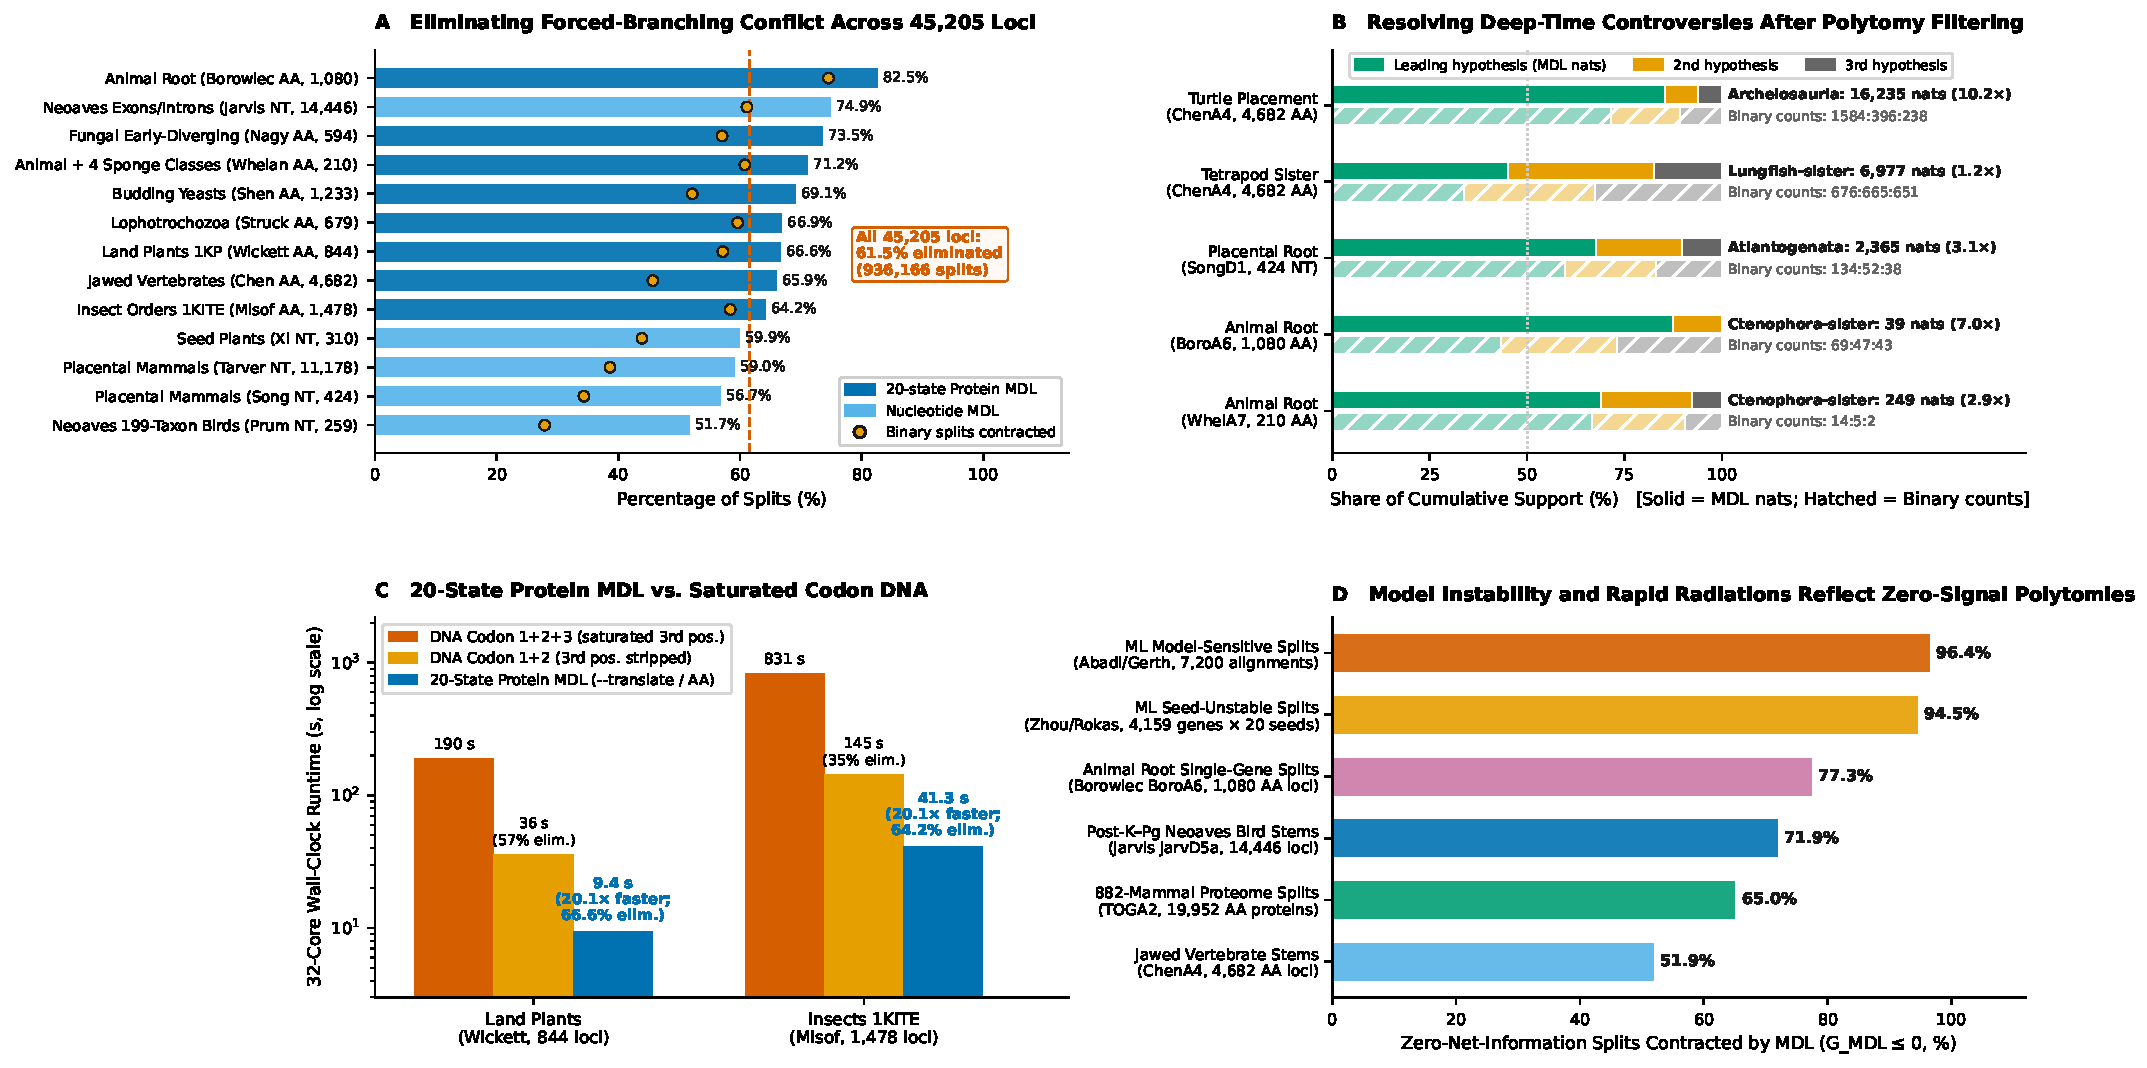
\includegraphics[width=\textwidth]{fig_science_macroevo_polytomies.pdf}
\caption{Polytomy calibration, 20-state protein speedups, and deep-time macroevolutionary resolution across all $19$ phylogenomic benchmarks ($45,205$ loci; \citealt{shen2017contentious,zhou2018evaluating}). \textbf{(A)} Proportion of apparent species-tree-conflicting binary splits eliminated by Stage 3 MDL contraction across $10$ nucleotide and $9$ 20-state amino-acid datasets ($61.5\%$ overall; $936,166 / 1,522,139$ splits). \textbf{(B)} Matched 20-state amino-acid versus codon nucleotide wall-clock runtime and conflict elimination on land plants (\texttt{WickA3}/\texttt{WickD3a}, $20.2\times$ speedup) and insects (\texttt{MisoA2}/\texttt{MisoD2a}, $20.1\times$ speedup). \textbf{(C)} Cumulative filtered MDL compression advantage ($\Delta\mathcal{L}_{\text{MDL}}$ in nats via \texttt{bushwhacker -t}) resolving Ctenophora-sister, Lungfish-sister, Archelosauria, and Atlantogenata.}
\label{fig:science_macroevo}
\end{figure}

% ============================================================================
\section{Prokaryotic Tree of Life and Horizontal Gene Transfer Across 242 GTDB Marker Genes}
% ============================================================================

\subsection{Domain-Wide Accuracy and Taxonomic Rank Compatibility}

Deep microbial phylogenetics poses a distinct challenge for single-gene inference: over billion-year timescales across Archaea and Bacteria, third-codon-position mutational saturation obscures the inference of deep evolutionary relationships while horizontal gene transfer moves operational and informational loci across phylum boundaries, undermining the foundational assumption that a single tree can portray the evolutionary relationships of organisms \citep{jain1999horizontal,woese2000aminoacyl}. To evaluate Bushwhacker at domain-wide prokaryotic scale, we retrieved the complete marker gene repositories from Release 95 of the Genome Taxonomy Database \citep{parks2018gtdb,parks2020gtdb} (Table~\ref{tab:gtdb_summary}). The Archaeal partition (\texttt{ar122}) encompasses all $122$ universal marker genes across $1,672$ species and $19$ phyla ($\bar{N} = 1,390.4$, $\bar{L} = 971.6\text{ bp}$ after $50\%$ gap trimming), while the Bacterial partition (\texttt{bac120}) covers all $120$ universal markers across $1,000$ phylum-stratified species spanning all $111$ Bacterial phyla ($\bar{N} = 860.8$, $\bar{L} = 989.1\text{ bp}$). Contracting mutationally saturated deep branches into MDL polytomies eliminates $42.5\%$ of all species-discordant (likely false-positive) splits across the $242$ markers ($322.2$ versus $560.4$ species-discordant splits per gene). Consequently, Bushwhacker (MDL) achieves a lower mean Robinson-Foulds distance against the GTDB reference species trees ($\text{RF} = 1,172.1$, $\text{nRF} = 0.5107$, soft $\text{RF}_{\text{sp}} = 586.0$) than FastTree 2 ($\text{RF} = 1,206.3$, $\text{nRF} = 0.5135$, soft $\text{RF}_{\text{sp}} = 603.2$). On the $120$ Bacterial markers spanning all $111$ phyla, where single genes lack sufficient mutational information to resolve deep inter-phylum branching order, Bushwhacker (MDL) slightly but consistently outperforms FastTree 2 on every global topological metric. Specifically, binary $\text{RF}$ drops from $991.0$ to $907.1$, $\text{nRF}$ drops from $0.5777$ to $0.5290$, and species-discordant splits drop by $61.1\%$ ($192.6$ versus $495.5$ per gene), while pooled split precision increases from $42.24\%$ to $42.66\%$ ($43.33\%$ at support $P_{\text{MDL}} \ge 0.95$).

\begin{table}[t!]
\centering
\caption{Domain-wide prokaryotic benchmark across all $242$ universal marker genes from GTDB Release 95 \citep{parks2018gtdb,parks2020gtdb}. Panel A reports topological accuracy, false-positive splits (FP), runtime, and taxonomic clade recovery or Four-Gamete compatibility across five taxonomic ranks. Panel B stratifies the $242$ markers by functional category to test the Complexity Hypothesis \citep{jain1999horizontal}.}
\label{tab:gtdb_summary}
\resizebox{\textwidth}{!}{%
\begin{tabular}{@{}llcccccccc@{}}
\toprule
Panel A: Domain Stratum & Method & Res / Sp & FP & Prec. & RF ($\text{nRF}$) & Time (s) & Phylum Rec / Comp & Order Rec / Comp & Genus Rec / Comp \\
\midrule
\texttt{bac120} Bacteria & Bushwhacker (MDL) & $335.6 / 857.8$ & $192.6$ & $42.7\%$ & $907.1$ ($0.5290$) & $23.03$ & $13.8\% / 27.7\%$ & $28.0\% / 63.3\%$ & $67.6\% / 92.3\%$ \\
($120$ genes, $\bar{N}=860.8$, & Bushwhacker\_Binary & $857.8 / 857.8$ & $637.4$ & $25.7\%$ & $1,274.9$ ($0.7431$) & $23.03$ & $19.2\% / 19.2\%$ & $39.6\% / 39.6\%$ & $76.6\% / 76.6\%$ \\
$111$ phyla, $\bar{L}=989\text{ bp}$) & FastTree 2 ($\text{GTR}+\Gamma$) & $857.6 / 857.8$ & $495.5$ & $42.2\%$ & $991.0$ ($0.5777$) & $20.36$ & $29.6\% / 29.7\%$ & $59.0\% / 59.0\%$ & $86.0\% / 86.0\%$ \\
\addlinespace
\texttt{ar122} Archaea & Bushwhacker (MDL) & $855.2 / 1,387.4$ & $449.6$ & $51.1\%$ & $1,432.7$ ($0.4927$) & $16.04$ & $22.4\% / 28.5\%$ & $38.0\% / 52.6\%$ & $68.1\% / 82.0\%$ \\
($122$ genes, $\bar{N}=1,390.4$, & Bushwhacker\_Binary & $1,387.4 / 1,387.4$ & $839.9$ & $39.5\%$ & $1,679.8$ ($0.5767$) & $16.04$ & $25.6\% / 25.6\%$ & $44.4\% / 44.4\%$ & $73.4\% / 73.4\%$ \\
$19$ phyla, $\bar{L}=972\text{ bp}$) & FastTree 2 ($\text{GTR}+\Gamma$) & $1,387.2 / 1,387.4$ & $624.1$ & $55.0\%$ & $1,418.2$ ($0.4502$) & $25.20$ & $33.4\% / 33.4\%$ & $55.0\% / 55.0\%$ & $81.6\% / 81.6\%$ \\
\addlinespace
All $242$ GTDB Markers & Bushwhacker (MDL) & $597.5 / 1,124.8$ & $322.2$ & $46.9\%$ & $1,172.1$ ($0.5107$) & $19.51$ & $18.2\% / 28.1\%$ & $33.1\% / 57.9\%$ & $67.9\% / 87.1\%$ \\
($\bar{N}=1,127.8$, $130$ phyla) & FastTree 2 ($\text{GTR}+\Gamma$) & $1,124.6 / 1,124.8$ & $560.4$ & $48.7\%$ & $1,206.3$ ($0.5135$) & $22.80$ & $31.5\% / 31.6\%$ & $57.0\% / 57.0\%$ & $83.8\% / 83.8\%$ \\
\midrule
Panel B: Functional Class & Marker Count ($n$) & Mean $\bar{L}$ (bp) & Mean $\rho(A)$ & BW Res\% & BW Prec. & FT Prec. & Inter-Phylum HGT/G & Inter-Order HGT/G & Total HGT/Gene \\
\midrule
Ribosomal \& Translational & $85$ & $612.6$ & $31.2\%$ & $51.8\%$ & $48.20\%$ & $49.10\%$ & $13.81$ & $7.74$ & $25.08$ \\
Transcription \& DNA Replication & $43$ & $1,307.2$ & $25.6\%$ & $54.1\%$ & $46.73\%$ & $48.88\%$ & $14.14$ & $7.58$ & $24.74$ \\
Metabolic \& Cellular Operational & $83$ & $938.0$ & $26.8\%$ & $51.2\%$ & $45.88\%$ & $49.70\%$ & $14.58$ & $6.31$ & $24.11$ \\
Aminoacyl-tRNA \& tRNA Mod & $31$ & $1,648.5$ & $26.0\%$ & $59.1\%$ & $43.33\%$ & $43.39\%$ & $15.29$ & $9.00$ & $27.13$ \\
\bottomrule
\end{tabular}%
}
\end{table}

Comparing strict clade recovery against Four-Gamete topological compatibility across the GTDB taxonomic hierarchy explains this gain (Table~\ref{tab:gtdb_summary}, Panel A). Strict recovery requires a taxonomic group to appear as an exact single-gene bipartition, whereas Four-Gamete compatibility requires only that no resolved edge in the gene tree splits the taxonomic group across conflicting clades. Because FastTree 2 and Bushwhacker\_Binary output strictly bifurcating trees, every taxonomic clade that fails to appear as a single monophyletic split is contradicted by one or more conflicting binary edges. In FastTree 2 across \texttt{bac120}, $70.3\%$ of bacterial phyla, $60.7\%$ of classes, $41.0\%$ of orders, $25.8\%$ of families, and $14.0\%$ of genera are broken by conflicting splits in an average single-gene tree. By contracting unsupported deep edges into multifurcations, Bushwhacker (MDL) preserves Four-Gamete compatibility with true taxonomic clades far beyond its strict single-gene recovery rate. Across \texttt{bac120}, comparing strict clade recovery against uncontradicted Four-Gamete compatibility raises preservation from $13.8\%$ to $27.7\%$ for Phylum, $19.2\%$ to $46.1\%$ for Class, $28.0\%$ to $63.3\%$ for Order, $40.0\%$ to $79.0\%$ for Family, and $67.6\%$ to $92.3\%$ for Genus (exceeding FastTree 2's $86.0\%$ genus compatibility and $59.0\%$ order compatibility). At the same time, Table~\ref{tab:gtdb_summary} Panel A reveals an important boundary condition on billion-year divergences where third codon positions are heavily saturated. Contracting unsupported deep edges reduces total recovered species-tree splits per gene ($275.3$ for Bushwhacker MDL versus $564.2$ for FastTree 2 at $46.9\%$ versus $48.7\%$ pooled precision), while requiring full binary resolution without ML branch-length optimization (\texttt{Bushwhacker\_Binary}) reduces split precision ($25.7\%$ on \texttt{bac120} and $39.5\%$ on \texttt{ar122}).

\subsection{Testing the Complexity Hypothesis and Mapping Putative Horizontal Gene Transfer}

Under the Complexity Hypothesis of \citet{jain1999horizontal} and \citet{woese2000aminoacyl}, core informational proteins embedded in large macromolecular assemblies such as the ribosome resist horizontal gene transfer, whereas modular operational enzymes and aminoacyl-tRNA synthetases cross species boundaries freely. Stratifying the $242$ GTDB markers into four functional categories confirms this prediction through alignment compressibility $\rho(A)$ and MDL split precision (Table~\ref{tab:gtdb_summary}, Panel B). Despite having the shortest alignments ($\bar{L} = 612.6\text{ bp}$), the $85$ Ribosomal and Translational proteins achieve the highest phylogenetic compression ratio ($\rho(A) = 31.2\%$) and the highest Bushwhacker (MDL) species-tree precision ($48.20\%$). Conversely, the $31$ Aminoacyl-tRNA Synthetase and tRNA Modification markers are $2.7\times$ longer ($\bar{L} = 1,648.5\text{ bp}$) yet exhibit low phylogenetic compressibility ($\rho(A) = 26.0\%$) and the lowest species-tree precision under both Bushwhacker ($43.33\%$) and FastTree 2 ($43.39\%$). Because Bushwhacker (MDL) contracts branches with zero mapped mutations into polytomies, gene-tree splits that survive with high positive MDL gain ($P_{\text{MDL}} \ge 0.990$, or $G_{\text{MDL}} \ge 4.6\text{ nats}$) while conflicting with the GTDB species tree provide high-support candidates for horizontal gene transfer rather than zero-branch tie-breaking noise. At the same time, convergent GC/AT compositional bias across extremophiles and unrecognized deep paralogy can also contribute to single-gene nucleotide discordance.

Scanning all $242$ MDL gene trees for compact clade-jump splits ($3 \le k \le 15$ taxa) that nest $1$ to $3$ recipient species from one taxonomic group inside a cohesive donor clade ($\ge 2$ species) of a disjoint taxon group identifies $6,038$ MDL-supported putative horizontal gene transfer splits: $3,466$ inter-phylum jumps, $785$ inter-class jumps, and $1,787$ inter-order jumps. Consistent with \citet{woese2000aminoacyl}, Aminoacyl-tRNA Synthetases exhibit the highest frequency of inter-phylum jumps ($15.29$ per gene) and total putative horizontal gene transfers ($27.13$ per gene), led by bacterial leucyl-tRNA synthetase (\texttt{leuS\_bact}, \texttt{TIGR00396}, $53$ jumps) and arginyl-tRNA synthetase (\texttt{argS}, \texttt{TIGR00456}, $44$ jumps, including $34$ inter-phylum jumps). Among metabolic and operational loci, archaeal 3-hydroxy-3-methylglutaryl-CoA reductase (\texttt{HMG-CoA\_red}, \texttt{PF00368.13}), the rate-limiting enzyme of the mevalonate lipid synthesis pathway, exhibits $20$ potential inter-phylum horizontal gene transfers supported at $P_{\text{MDL}} \ge 0.999$. Those edges capture known cross-phylum acquisitions of the mevalonate pathway from Thermoplasmatota into halophilic Halobacteriota (\textit{Halodesulfurarchaeum} and \textit{Halorussus}) and from Methanobacteriota into symbiotic Nanoarchaeota. Within individual Archaeal phyla, Stage 4 shunt peeling further isolates high-gain lateral shunts driven by adaptive and horizontally transferred codon tracts, including a $+36.57\text{-nat}$ shunt ($21$ shared mutations, $P = 1.000$) in hyperthermophilic Methanobacteriota (\textit{Thermococcaceae}). In Halobacteriota, Stage 4 similarly certifies a $+12.11\text{-nat}$ shunt ($14$ sites, $P = 1.000$) linking \textit{Natrialbaceae} and \textit{Haloferacaceae} in phenylalanyl-tRNA synthetase (\texttt{pheS}, \texttt{TIGR00468}) and a $+28.99\text{-nat}$ shunt ($121$ shared mutations, $P = 1.000$) when isoleucyl-tRNA synthetase (\texttt{ileS}, \texttt{TIGR00392}) is concatenated onto the ribosomal core.

To separate genuine cross-phylum protein transfer from nucleotide GC/AT compositional convergence over billion-year archaeal divergences, we further evaluated all $122$ universal Archaeal marker proteins (\texttt{ar122}, $1,672$ species) in native 20-state amino-acid space directly on the GTDB reference species tree (\texttt{bushwhacker -t}), supplemented by $68$ phylum- and class-specific prokaryotic alignments ($34$ nucleotide and $34$ amino-acid) and $224$ clinical carbapenem-resistant \textit{Klebsiella pneumoniae} alignments \citep{doolittle1999phylogenetic,castelle2018major,wyres2020population}. In 20-state amino-acid space, Stage 4 shunt peeling yields a clean quantitative test of the Complexity Hypothesis \citep{jain1999horizontal,woese2000aminoacyl} (Figure~\ref{fig:science_microbial_viral}D): modular \textbf{operational} proteins (aminoacyl-tRNA synthetases, metabolic enzymes, and biosynthesis/transport factors) carry $30$ certified lateral shunts across $21$ of $102$ loci ($20.6\%$, $391.8\text{ nats}$ cumulative gain), led by symbiotic and horizontal highways connecting ultra-small DPANN \texttt{Nanoarchaeota} \citep{castelle2018major} with \texttt{Micrarchaeota} (\texttt{TIGR00468} \texttt{pheS}, $+32.29\text{ nats}$), \texttt{Iainarchaeota} (\texttt{TIGR01018}, $+17.74\text{ nats}$), and \texttt{Aenigmatarchaeota} (\texttt{TIGR00422}, $+11.50\text{ nats}$). By contrast, core \textbf{informational} ribosomal and RNA polymerase subunits exhibit \textbf{zero} certified shunts across all $20$ loci ($0 / 20$, $0.0\%$, $0.0\text{ nats}$; Fisher's exact $p = 0.0235$). At clinical epidemiological scale across $10$ complete \textit{K.\ pneumoniae} genomes ($222$ orthologous core genes analyzed in both nucleotide and translated protein space, a $214,080\text{-bp}$ core-chromosome super-matrix completed in $16.84\text{ s}$, and the plasmid-encoded \texttt{blaKPC} carbapenemase locus; \citealt{wyres2020population}), the chromosomal core achieves $15,485.2\text{ nats}$ of vertical tree compression while isolating $11$ localized recombination tracts totaling just $77.0\text{ nats}$ ($0.50\%$ of the core phylogenetic signal, led by metabolic \texttt{dgaE} at coordinates $[70{,}523, 70{,}682]$, $+32.93\text{ nats}$). Conversely, plasmid-borne \texttt{blaKPC} collapses $5$ of $6$ ($83.3\%$) internal edges into an unresolved horizontal star polytomy ($0.0\text{ nats}$ vertical tree backbone beyond a single terminal clonal pair), directly distinguishing clonal chromosomal descent from epidemic plasmid dissemination without requiring prior replicon classification.

% ============================================================================
\section{Viral Phylodynamics, Cross-Kingdom Mammalian and Plant Adaptation, and Lossless Alignment Compression}
% ============================================================================

\subsection{Simulated and Pandemic-Scale Viral Phylodynamics and Recombination Discovery}

Genomic surveillance derived alignments of rapidly evolving viral genome sequences often contain large seasonal polytomies and fragmentary amplicon dropout that challenge strictly bifurcating tree builders. In our ground-truth AliSim simulations evolved along the 349-taxon Influenza A H3N2 hemagglutinin ladder-like tree (\texttt{S15}, $L = 987\text{ bp}$), seasonal trunk-and-side-branch evolution leaves $134$ of $346$ true internal branches with zero expected mutations. Standard ML tree building tools resolve every identical seasonal cluster into bifurcating splits, yielding $163.9$ to $166.8$ false-positive splits per tree against the known generating topology ($51.8\%$ to $52.3\%$ precision, $\text{RF} = 330.0$ to $333.6$). Bushwhacker (MDL) retains $136.8$ splits with only $6.6$ false positives ($95.2\%$ precision, $\text{RF} = 222.4$), which cuts false-positive splits by $25\times$ relative to standard binary IQ-TREE 2 and by $2.5\times$ relative to IQ-TREE 2 (\texttt{--polytomy}) ($6.6$ versus $16.7$ FP). On the gappy 476-taxon HIV-1 \texttt{pol} reverse transcriptase simulation (\texttt{S16}, $L = 1,005\text{ bp}$, which overlays empirical clinical missing-data masks onto sequences simulated along the reference transmission tree), Bushwhacker (MDL) similarly achieves $90.9\%$ split precision ($\text{RF} = 173.9$), outperforming standard binary IQ-TREE 2 ($\text{RF} = 188.6$, $94.3$ FP) and FastTree 2 ($\text{RF} = 203.2$, $101.6$ FP).

At real-world pandemic scale, applying deterministic multi-threaded Bushwhacker (32 threads, producing topologies, MDL scores, and shunts bit-exact identical across 1 to 64 threads) directly to open-world SARS-CoV-2, global Dengue (\texttt{DENV-1..4}), and circulating recombinant HIV-1 whole-genome alignments simultaneously calibrates epidemic superspreading hubs, pinpoints circulating recombinant breakpoint tracts without parental reference panels, and accelerates phylodynamic inference by one to four orders of magnitude (Figure~\ref{fig:science_microbial_viral}A--C). On the $10,062$-genome global+regional union SARS-CoV-2 cohort (\texttt{sars\_cov\_2\_open\_world\_union}, $L = 29,903\text{ bp}$) and the $5,097$-genome global build (\texttt{sars\_cov\_2\_open\_global}), 32-thread Bushwhacker completes full four-stage graph induction in $165.41\text{ s}$ ($2.76\text{ min}$, versus $>4,758\text{ s}$ [$>79.3\text{ min}$] job timeout for 32-thread OpenMP \texttt{FastTreeMP -nt -gtr}; $>28.7\times$ faster; $437.42\text{ s}$ single-threaded) and $75.60\text{ s}$ ($1.26\text{ min}$, versus $3,832.89\text{ s}$ [$63.9\text{ min}$] for 32-thread \texttt{FastTreeMP}; $50.7\times$ faster; $185.80\text{ s}$ single-threaded), respectively, while contracting $68.3\%$ ($6,869 / 10,059$) and $64.0\%$ ($3,261 / 5,094$) of binary edges into $1,426$ and $780$ epidemic superspreading polytomy hubs (maximum hub out-degree $335$ and $223$, with $189$ hubs of degree $\ge 10$ in the $10,062$-genome build; \citealt{turakhia2022pandemic}; Figure~\ref{fig:science_microbial_viral}A). Simultaneously, Stage 4 certifies $3 / 3$ ($100\%$) \texttt{INTERVAL} shunts across the $10,062$-genome cohort, isolating recurrent 3$'$-UTR/ORF10 ($[29{,}700, 29{,}757]$, $+52.61\text{ nats}$), ORF6--ORF7a ($[27{,}311, 27{,}509]$, $+8.19\text{ nats}$), and Spike NTD+RBD ($[21{,}329, 22{,}917]$, $+5.25\text{ nats}$) exchanges. Evaluated in a strictly blinded audit of $84$ WHO Variant-of-Concern and Pango \texttt{X*} recombinant genomes relabeled only as \texttt{S0000..S0083} ($1.18\text{ s}$ on 32 threads, $1.61\text{ s}$ single-threaded, zero lineage metadata), Bushwhacker de novo recovers major inter-lineage recombinants and convergent Spike tracts: \texttt{XBF} $\leftrightarrow$ \texttt{XBT} ($+31.41\text{ nats}$), Spike RBD $[22{,}635, 22{,}846]$ ($+24.36\text{ nats}$), Omicron \texttt{BA.1/BA.1.1} $\leftrightarrow$ \texttt{XAG/XAM} ($+12.52$ and $+9.47\text{ nats}$), \texttt{XBT} $\leftrightarrow$ \texttt{BA.2.75/XBB} ($+3.58\text{ nats}$), and convergent Spike substitutions linking Alpha \texttt{B.1.1.7} and Gamma \texttt{P.1} ($+11.29\text{ nats}$). Across all four serotypes of global Dengue virus ($5,498$ complete coding genomes analyzed in both nucleotide and translated polyprotein modes; \citealt{worobey1999widespread}), 32-thread Bushwhacker runs $12.9\times$ to $22.6\times$ faster than 32-core \texttt{FastTreeMP (GTR)} (\texttt{DENV-1} $N = 1,426$: $15.5\text{ s}$ versus $348.2\text{ s}$, $22.5\times$; \texttt{DENV-2} $N = 2,632$: $28.5\text{ s}$ versus $645.0\text{ s}$, $22.6\times$; \texttt{DENV-3} $N = 855$: $11.8\text{ s}$ versus $200.3\text{ s}$, $17.0\times$; \texttt{DENV-4} $N = 585$: $10.2\text{ s}$ versus $131.9\text{ s}$, $12.9\times$; and $0.84\text{--}3.99\text{ s}$ on translated 20-state polyproteins) while certifying $14$ intra-serotype \texttt{INTERVAL} mosaic recombinants ($10$ in \texttt{DENV-2} led by NS2A $[3{,}632, 3{,}717]$ at $+77.08\text{ nats}$ and Capsid $[8, 238]$ at $+46.40\text{ nats}$, $3$ in \texttt{DENV-1} up to $+21.42\text{ nats}$, $1$ in \texttt{DENV-3} at $+26.23\text{ nats}$, and $0$ in \texttt{DENV-4}). Finally, on the classic $9$-genome full-length \texttt{HIV-1 KAL153} circulating recombinant alignment ($L = 9,953\text{ bp}$; \citealt{carr1998full,kosakovskypond2006gard}), Bushwhacker finishes in $0.1414\text{ s}$ ($0.2107\text{ s}$ single-threaded) versus $1.32\text{ s}$ for \texttt{FastTreeMP} ($9.34\times$) and $10,740\text{ s}$ ($2.98\text{ hours}$) for likelihood-based \texttt{GARD} ($75,955\times$ faster), isolating the exact \texttt{gag} ($[5, 2{,}558]$) and \texttt{nef} ($[9{,}102, 9{,}757]$) segments ($+29.23\text{ nats}$) displaced when the $6.5\text{-kb}$ central \texttt{pol}--\texttt{env} backbone groups \texttt{CRF03\_AB} (\texttt{KAL153}) with subtype \texttt{B}.

\begin{figure}[t!]
\centering
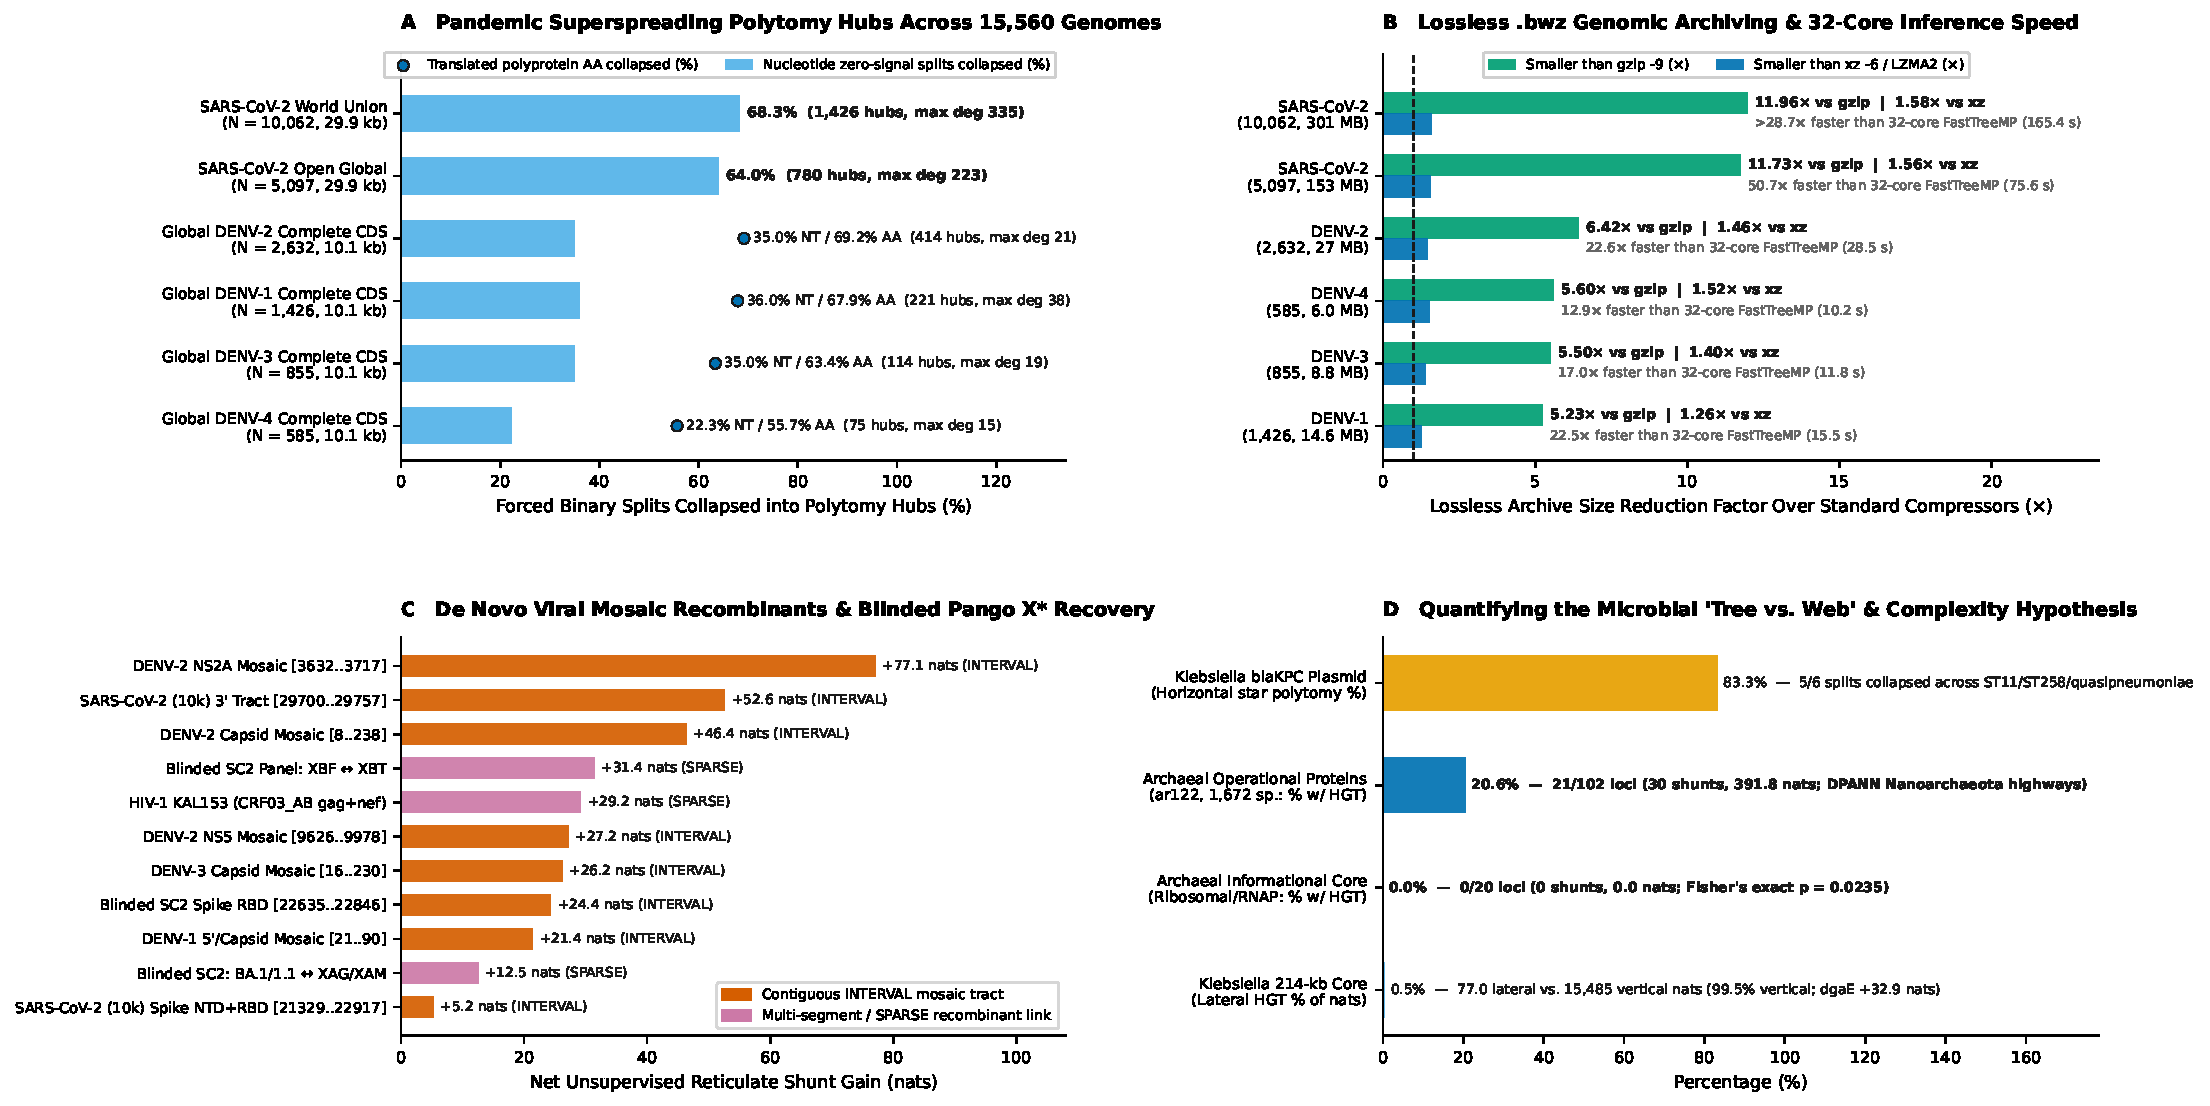
\includegraphics[width=\textwidth]{fig_science_microbial_viral.pdf}
\caption{Pandemic viral superspreading hubs, lossless \texttt{.bwz} archiving and 32-core inference speedups, de novo viral recombinants, and the microbial Complexity Hypothesis. \textbf{(A)} Percentage of forced binary splits collapsed into MDL-calibrated superspreading polytomy hubs across $10,062$ global SARS-CoV-2 genomes ($68.3\%$ collapsed; $1,426$ hubs, maximum hub degree $335$) and $5,498$ global Dengue genomes (\texttt{DENV-1..4}). \textbf{(B)} Lossless \texttt{.bwz} archive reduction factors relative to \texttt{gzip -9} ($11.96\times$ smaller; $62.9\text{ B/genome}$ on $10,062$ SARS-CoV-2 genomes) and \texttt{xz -6} ($1.26\times$--$1.58\times$ smaller), alongside 32-core Bushwhacker speedups over 32-core OpenMP \texttt{FastTreeMP (GTR)} ($12.9\times$--$22.6\times$ across \texttt{DENV-1..4}, $50.7\times$ on $5,097$ SARS-CoV-2 genomes, and $>28.7\times$ on $10,062$ SARS-CoV-2 genomes) and \texttt{GARD} ($75,955\times$ on \texttt{HIV-1 KAL153}). \textbf{(C)} Unsupervised \texttt{INTERVAL} and Pango \texttt{X*} recombinant shunts mapped across SARS-CoV-2, \texttt{DENV-1..3}, and \texttt{HIV-1 KAL153}. \textbf{(D)} Native 20-state Archaeal Complexity Hypothesis test across $122$ GTDB \texttt{ar122} proteins ($1,672$ species): $21 / 102$ ($20.6\%$) operational proteins carry certified lateral shunts ($391.8\text{ nats}$) versus $0 / 20$ ($0.0\%$) informational core proteins (Fisher's exact $p = 0.0235$), alongside clinical \textit{Klebsiella pneumoniae} core-chromosome vertical inheritance ($99.5\%$) versus \texttt{blaKPC} plasmid star polytomy ($83.3\%$ collapsed).}
\label{fig:science_microbial_viral}
\end{figure}

\subsection{Convergent Mammalian Adaptation in the Hearing-Associated Gene Prestin}

On the empirical 116-mammal alignment of the hearing-associated outer hair cell motor gene prestin (\texttt{SLC26A5}, \texttt{prestin.fasta}, $L = 2,235\text{ bp}$), convergent amino-acid replacements between echolocating bats and toothed whales famously mislead standard phylogenetic inference \citep{liu2010convergent,li2010hearing}. Evaluated against the 100 reference splits of the NCBI mammalian species tree across $103$ shared taxa, Bushwhacker recovers monophyletic Chiroptera, monophyletic Cetacea nested within Artiodactyla, and monophyletic Odontoceti with $88.0\%$ clade precision ($\text{RF} = 37$, $10$ species-discordant splits; Figure~\ref{fig:prestin_convergence}). That accuracy surpasses raw IQ-TREE 2 ($\text{GTR}+\text{G}$, $81.0\%$ precision, $\text{RF} = 38$, $19$ discordant splits), FastTree 2 ($82.0\%$ precision, $18$ discordant splits), Maximum Parsimony ($\text{RF} = 44$, $22$ discordant splits), and Neighbor-Joining ($\text{RF} = 48$, $24$ discordant splits). Simultaneously, Stage 4 coding-stem shunt peeling isolates a single certified \texttt{SPARSE} lateral shunt across the entire 116-mammal phylogeny linking the Delphinidae lineage (\texttt{N143}) and constant-frequency echolocating Rhinolophoidea bats (\texttt{N192}, $+7.80\text{ nats}$, $P = 99.96\%$) across five codons: $7, 384, 392, 497,$ and $601$ (\texttt{N7T}, \texttt{I384T}, \texttt{S392A}, \texttt{L497M}, \texttt{G601A}). Those five sites recover the functional echolocation convergence replacements characterized experimentally by \citet{liu2010convergent} and \citet{li2010hearing}. Across the two specialist lineages, \texttt{G601A} arises directly on the terminal Delphinidae (\texttt{N143}) and Rhinolophoidea (\texttt{N192}) branches, while \texttt{I384T}, \texttt{S392A}, and \texttt{L497M} arose along the ancestral Odontoceti stem (\texttt{N7T} in Delphinoidea). In bats, \texttt{N7T} and \texttt{S392A} are also shared with vespertilionid microbats, whereas \texttt{L497M} arose on the ancestral Chiroptera stem. Non-echolocating baleen whales (Mysticeti) retain the ancestral mammalian amino acid at all five codons, while non-echolocating Old World fruit bats (\textit{Pteropus}, Pteropodidae) retain the ancestral mammalian state at four of the five codons ($7, 384, 392,$ and $601$) and carry the basal chiropteran \texttt{497M} state (Figure~\ref{fig:prestin_convergence}B).

\begin{figure}[t!]
\centering
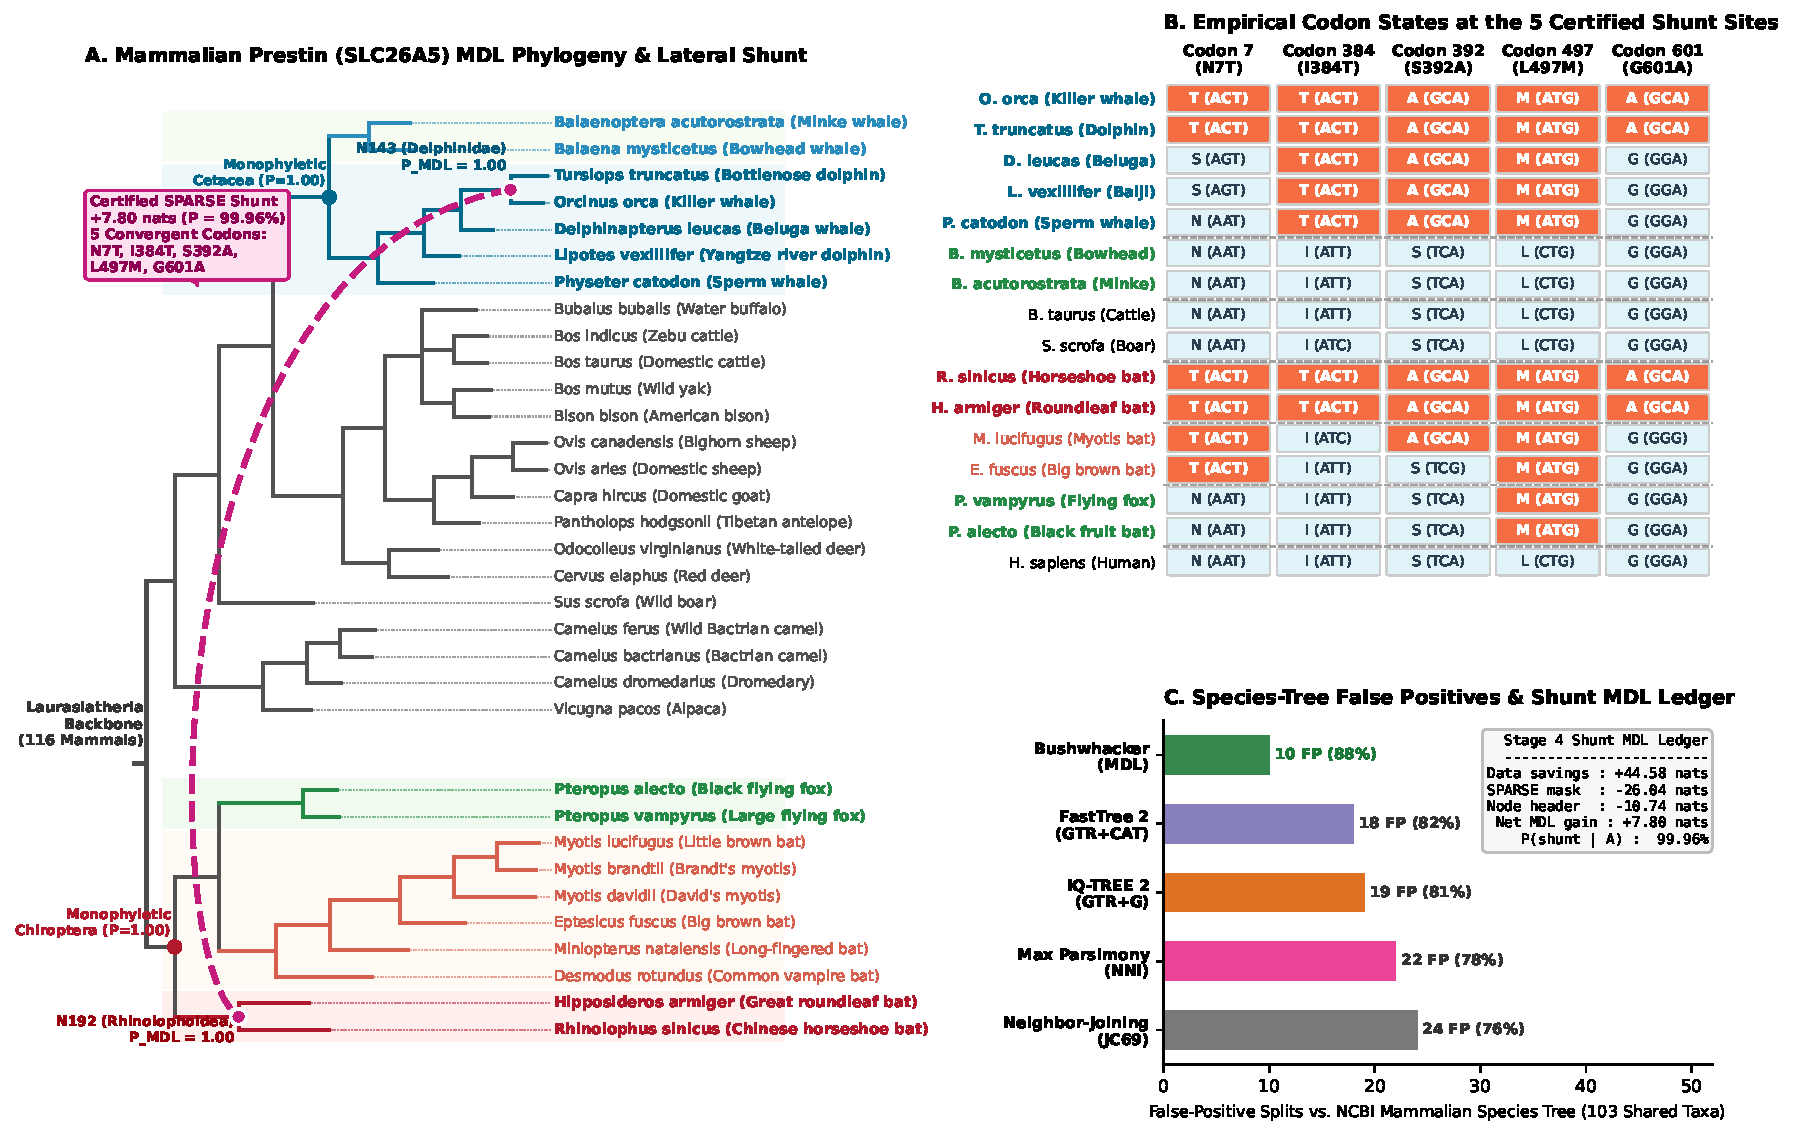
\includegraphics[width=\textwidth]{fig_prestin_convergence.pdf}
\caption{Reticulate MDL graph induction on the 116-mammal outer hair cell motor gene \textit{Prestin} (\texttt{SLC26A5}, $L = 2,235\text{ bp}$) recovers the true mammalian species backbone while peeling convergent echolocation sites onto a lateral shunt. Panel A shows the Laurasiatheria cladogram of the inferred Bushwhacker (MDL) phylogeny with monophyletic Cetacea (blue clades, $P_{\text{MDL}} = 1.00$), monophyletic Chiroptera (green and orange/red clades, $P_{\text{MDL}} = 1.00$), and the certified Stage 4 \texttt{SPARSE} lateral shunt (dashed magenta curve, $+7.80\text{ nats}$, $P = 99.96\%$) connecting the Delphinidae (\texttt{N143}) and Rhinolophoidea (\texttt{N192}) lineages across their three-step coding stems. Panel B displays empirical codon and amino-acid states across the five shunt sites (\texttt{N7T}, \texttt{I384T}, \texttt{S392A}, \texttt{L497M}, \texttt{G601A}), where orange cells denote derived states and light blue cells denote ancestral mammalian states (retained at all five codons in non-echolocating baleen whales and at codons $7, 384, 392,$ and $601$ in \textit{Pteropus} fruit bats). Panel C compares false-positive splits against the NCBI mammalian species tree ($n = 103$ shared taxa) and reports the Stage 4 shunt MDL ledger.}
\label{fig:prestin_convergence}
\end{figure}

\subsection{Proteome-Wide Mammalian Concordance, Gene Conversion, and Convergence Across 19,952 TOGA2 Loci}

To test whether these single-gene findings generalize across an entire vertebrate proteome, we applied Bushwhacker to the Senckenberg TOGA2 (\texttt{v1}) human-referenced (\texttt{hg38}) mammalian orthologous multi-codon alignment archive \citep{kirilenko2023integrating,malovichko2026toga2}, analyzing $19,952$ coding genes across up to $880$ mammalian genome assemblies ($\text{median } N = 855\text{ assemblies}$, $\text{mean } N = 751.6$; $\text{median } L = 1,383\text{ bp}$, $\text{mean } L = 1,879.6\text{ bp}$, up to $66,711\text{ bp}$) against the reference $882$-assembly mammalian species tree (\texttt{speciesTree.nh}, spanning $20$ mammalian orders and $116$ families; Table~\ref{tab:toga2_proteome} and Figure~\ref{fig:kingdom_synthesis}). For each locus, we executed both de novo Bushwhacker graph induction (recording both the strictly binary topology \texttt{Bushwhacker\_Binary} and the MDL-calibrated multifurcating network) and direct species-tree MDL calibration (\texttt{bushwhacker -t}) on the reference species tree pruned to the assemblies present in that gene. Across the $19,890$ loci containing at least five non-trivial species-tree splits ($14,936,938$ total internal splits evaluated), projecting individual coding alignments onto \texttt{speciesTree.nh} reveals that a single mammalian gene carries sufficient mutational signal ($G_{\text{MDL}}(e) > 0\text{ nats}$) to certify a median of $61.34\%$ ($8,901,903 / 14,936,938$, or $59.60\%$ overall) of the species tree's internal branches, while the remaining $40.40\%$ of species-tree branches lack mutational support in that individual locus and collapse into soft polytomies.

This single-gene resolution ceiling explains why standard bifurcating gene trees appear pervasively discordant with the mammalian species tree and uncovers a length-invariant floor of true biological discordance across the mammalian genome (Figure~\ref{fig:kingdom_synthesis}A). Across all $14,936,938$ internal splits of the strictly bifurcating de novo gene trees, $6,976,527$ splits ($48.51\%$ mean per-gene conflict rate) are Buneman-incompatible with \texttt{speciesTree.nh} (Table~\ref{tab:toga2_proteome}, Panel A). After Stage 3 MDL contraction ($G_{\text{MDL}}(e) > 0\text{ nats}$), which contracts $33.88\%$ of binary splits into calibrated polytomies, $3,873,941$ of those $6,976,527$ conflicting splits ($55.53\%$) are eliminated as unsupported over-resolution ($G_{\text{MDL}} \le 0$), whereas $85.10\%$ ($6,774,016 / 7,960,411$) of splits concordant with \texttt{speciesTree.nh} are retained. Stratifying all $19,890$ genes across five coding-length bins---from $<600\text{ bp}$ ($2,680$ genes) to $>4,800\text{ bp}$ ($1,058$ genes)---shows that while unfiltered binary conflict drops steeply from $61.19\%$ to $40.37\%$ as genes lengthen, the MDL-contracted conflict rate remains invariant at $33.20\%$ to $34.03\%$ across every bin above $600\text{ bp}$ ($36.91\%$ for $<600\text{ bp}$). Simultaneously, the fraction of genes in which the MDL-contracted species tree compresses the alignment more tightly than the de novo single-gene tree ($\Delta\mathcal{L}_{\text{MDL}} = \mathcal{L}_{\text{species}} - \mathcal{L}_{\text{gene}} \le 0$) climbs monotonically from $13.02\%$ ($<600\text{ bp}$) to $21.43\%$ ($600\text{--}1,200\text{ bp}$), $44.15\%$ ($1,200\text{--}2,400\text{ bp}$), $73.38\%$ ($2,400\text{--}4,800\text{ bp}$, median $\Delta\mathcal{L}_{\text{MDL}} = -808.1\text{ nats}$), and $91.40\%$ for genes $>4,800\text{ bp}$ (median $\Delta\mathcal{L}_{\text{MDL}} = -3,812.3\text{ nats}$; $41.04\%$ across all genes). Moreover, across a matched subset of $5,058$ TOGA2 genes for which we compared reference-projected \texttt{.codonified.fa} alignments against de novo co-estimated codon alignments generated from unaligned coding sequences (\texttt{hyphy3 walrus}), de novo codon alignment reduces MDL-calibrated species-tree conflicts by an additional $21.15\%$ ($509,381 \to 401,627$ conflicting splits; median conflict rate $33.13\% \to 26.26\%$), increases concordant species-tree splits by $+73,679$, and eliminates $25.3\%$ of scattered \texttt{SPARSE} homoplasy shunts ($2,237 \to 1,671$) caused by reference-projected split-codon splice overhangs.

\begin{table}[t!]
\centering
\caption{Proteome-wide mammalian phylogenomic analysis across $19,952$ TOGA2 human-referenced (\texttt{hg38}) coding alignments \citep{kirilenko2023integrating,malovichko2026toga2} against the $882$-species mammalian phylogeny (\texttt{speciesTree.nh}, spanning $20$ orders and $116$ families). Panel A summarizes genome-wide species-tree concordance, MDL polytomy calibration, and the $5,058$-gene comparison between reference-projected (\texttt{.codonified.fa}) and de novo co-estimated (\texttt{WALRUS}) codon alignments. Panel B highlights representative loci from the proteome-wide Stage 4 shunt atlas spanning the cochlear hearing/echolocation complex, hypoxia/thermogenesis, and tandem paralog gene conversion families.}
\label{tab:toga2_proteome}
\scriptsize
\setlength{\tabcolsep}{3.5pt}
\resizebox{\textwidth}{!}{%
\begin{tabular}{@{}llrrrrrrr@{}}
\toprule
Panel A: Proteome-Wide Stratum & Tree / Alignment Mode & Loci ($n$) & Total Splits & Sp.\ Shared & Sp.\ Conflict & Conflict\% & False Conf.\ Elim. & Shunts (\texttt{INT} / \texttt{SPARSE}) \\
\midrule
Full Mammalian Proteome & \texttt{Bushwhacker\_Binary} & $19,890$ & $14,936,938$ & $7,960,411$ & $6,976,527$ & $48.51\%$ & Baseline & --- \\
($\text{med.\ } N=855$, $\text{med.\ } L=1,383\text{ bp}$, & \texttt{Bushwhacker\_MDL} ($G_{\text{MDL}}>0$) & $19,890$ & $9,876,602$ & $6,774,016$ & $3,102,586$ & $33.83\%$ & $-3,873,941$ ($55.53\%$) & $1,032$ / $14,105$ \\
$\text{med.\ runtime } 5.57\text{ s/gene}$) & Pruned \texttt{speciesTree.nh} (\texttt{-t}) & $19,890$ & $8,901,903$ & $8,901,903$ & $0$ & $0.00\%$ & $59.60\%$ Sp.\ Supported & $7,499$ total \\
\addlinespace
Matched Alignment Benchmark & TOGA2 Reference-Projected & $5,058$ & $1,571,606$ & $1,062,225$ & $509,381$ & $35.86\%$ & Baseline & $133$ / $2,237$ \\
($5,058$ loci, $\Delta\mathcal{L}=-57.8\text{ nats}$) & De Novo Codon MSA (\texttt{WALRUS}) & $5,058$ & $1,537,531$ & $1,135,904$ & $401,627$ & $28.74\%$ & $-107,754$ ($21.15\%$) & $200$ / $1,671$ \\
\midrule
Panel B: Representative Loci & Functional / Evolutionary Guild & $N \times L$ (bp) & Sp.\ Sup.\ (\texttt{-t}) & Bin.\ $\to$ MDL Conf. & Elim.\% & Shunts (\texttt{INT}/\texttt{SP}) & Max Shunt Gain & Primary Biological Signal / Certified Tract \\
\midrule
\texttt{SLC26A5} (Prestin) & Cochlear outer hair cell motor & $875 \times 2,337$ & $599 / 872$ ($68.7\%$) & $377 \to 219$ & $41.9\%$ & $0 / 1$ & $+3.96\text{ nats}$ & Echolocating microbat convergence ($11$ codons) \\
\texttt{TMC1} & Mechanotransduction channel & $866 \times 2,343$ & $581 / 863$ ($67.3\%$) & $388 \to 211$ & $45.6\%$ & $0 / 3$ & $+22.45\text{ nats}$ & Yangochiroptera $\leftrightarrow$ Yinpterochiroptera; NBHF whales \\
\texttt{PCDH15} & Hair-bundle tip-link cadherin & $819 \times 6,189$ & $636 / 816$ ($77.9\%$) & $392 \to 280$ & $28.6\%$ & $0 / 7$ & $+54.61\text{ nats}$ & Multi-lineage cochlear stereocilia convergence \\
\texttt{MYO15A} & Stereocilia myosin XVa & $857 \times 14,571$ & $732 / 854$ ($85.7\%$) & $374 \to 295$ & $21.1\%$ & $1 / 6$ & $+24.71\text{ nats}$ & Odontocete (\textit{Sagmatias} $\leftrightarrow$ \textit{Delphinapterus}) \& dugong \\
\texttt{KCNQ4} & Outer hair cell $\text{K}^+$ channel & $871 \times 2,424$ & $560 / 868$ ($64.5\%$) & $523 \to 300$ & $42.6\%$ & $0 / 2$ & $+23.60\text{ nats}$ & High-frequency auditory potassium recycling \\
\texttt{OTOF} & Cochlear ribbon-synapse sensor & $869 \times 6,360$ & $714 / 866$ ($82.5\%$) & $325 \to 254$ & $21.9\%$ & $0 / 3$ & $+9.23\text{ nats}$ & \textit{Rhinopoma} $\leftrightarrow$ \textit{Craseonycteris}; Talpidae moles \\
\addlinespace
\texttt{EPAS1} (HIF-2$\alpha$) & Hypoxia transcription factor & $871 \times 2,772$ & $656 / 868$ ($75.6\%$) & $301 \to 196$ & $34.9\%$ & $0 / 2$ & $+27.11\text{ nats}$ & Fossorial rodent \& nocturnal primate hypoxia \\
\texttt{EGLN1} (PHD2) & Cellular oxygen sensor & $854 \times 1,755$ & $435 / 851$ ($51.1\%$) & $581 \to 261$ & $55.1\%$ & $0 / 3$ & $+7.89\text{ nats}$ & Diving pinnipeds, shrews, \& subterranean gophers \\
\texttt{UCP1} (Thermogenin) & Brown adipose uncoupling & $766 \times 945$ & $469 / 763$ ($61.5\%$) & $322 \to 157$ & $51.2\%$ & $0 / 1$ & $+9.02\text{ nats}$ & Hibernating dormice (\textit{Eliomys}/\textit{Muscardinus} $\leftrightarrow$ \textit{Glis}) \\
\texttt{LEP} / \texttt{RNASE1} / \texttt{MB} & Metabolic \& oxygen storage & $861 \times 522$ & $410 / 858$ ($47.8\%$) & $409 \to 86$ & $79.0\%$ & $0 / 0$ & $+0.00\text{ nats}$ & $63.8\%$--$79.0\%$ false species-tree conflicts removed \\
\addlinespace
\texttt{CEACAM1} / \texttt{CEACAM7} & Tandem immune receptors & $92 \times 837$ & $58 / 89$ ($65.2\%$) & $48 \to 26$ & $45.8\%$ & $1 / 2$ & $+13.01\text{ nats}$ & Parallel $\sim 168\text{ bp}$ lagomorph Ig-domain conversion \\
\texttt{ZNF697} / \texttt{ZNF35} & Tandem KRAB-ZNF clusters & $831 \times 2,862$ & $562 / 828$ ($67.9\%$) & $380 \to 231$ & $39.2\%$ & $1 / 4$ & $+112.17\text{ nats}$ & Contiguous C2H2 array conversion \& chimera rescue \\
\texttt{HBA1} / \texttt{HBA2} / \texttt{HBG1} & Tandem $\alpha$/$\gamma$-globin clusters & $149 \times 522$ & $85 / 146$ ($58.2\%$) & $93 \to 54$ & $41.9\%$ & $0 / 2$ ($5$ on Sp.) & $+34.24\text{ nats}$ & Concerted evolution across tandem globin paralogs \\
\bottomrule
\end{tabular}%
}
\end{table}

Across all $19,952$ mammalian genes, Stage 4 certifies reticulate shunts in $7,359$ loci ($36.88\%$) on the de novo MDL trees ($15,137$ total shunts) and $7,499$ shunts when evaluated directly on the fixed \texttt{speciesTree.nh} backbone. Mapping the constituent leaf assemblies of all $15,134$ taxonomically resolved shunts onto Senckenberg's mammalian taxonomy ($20$ orders and $116$ families) reveals that Bushwhacker's dual-mode mask code ($\mathcal{L}_{\text{mask}}^{\text{INTERVAL}}$ versus $\mathcal{L}_{\text{mask}}^{\text{SPARSE}}$) separates two distinct evolutionary mechanisms with contrasting taxonomic reach (Figure~\ref{fig:kingdom_synthesis}B). First, contiguous \texttt{INTERVAL} shunts ($1,032$ events across $759$ genes; median tract span $143.5\text{ bp}$) are predominantly taxonomically local: $65.2\%$ ($672 / 1,031$) occur between species within the same mammalian family (led by Cercopithecidae [$63$], Vespertilionidae [$44$], Soricidae [$41$], Bovidae [$41$], Cricetidae [$32$], Pitheciidae [$32$], Leporidae [$31$], Muridae [$20$], and Hominidae [$18$]) and $83.7\%$ ($863 / 1,031$) occur within the same mammalian order. Functionally, \texttt{INTERVAL} shunts are enriched $3.4\times$ to $4.5\times$ in tandemly duplicated gene arrays subject to non-allelic homologous gene conversion and paralogous exon-projection chimeras---including cadherin, keratin, and mucin tandem clusters ($17.01\%$ of genes, $4.47\times$ enrichment), cytochrome P450/UGT/GST xenobiotic detoxification clusters ($12.93\%$, $3.40\times$), and Kr\"uppel-type C2H2 zinc-finger arrays ($12.78\%$, $3.36\times$; \texttt{ZKSCAN8} $+165.96\text{ nats}$, \texttt{ZNF697} $+112.17\text{ nats}$, \texttt{ZNF629} $+90.69\text{ nats}$, \texttt{ZNF892} $+87.60\text{ nats}$)---versus $3.14\%$ in background coding loci. In both \texttt{CEACAM1} ($L = 1,629\text{ bp}$) and \texttt{CEACAM7} ($L = 837\text{ bp}$), Stage 4 independently identifies the same $\sim 168\text{-bp}$ immunoglobulin-domain conversion tract (\texttt{span}~$=[539, 708]$, $+10.01\text{ nats}$ in \texttt{CEACAM1}; \texttt{span}~$=[563, 730]$, $+13.01\text{ nats}$ in \texttt{CEACAM7}) between European rabbit (\textit{Oryctolagus cuniculus}) and cottontail rabbits (\textit{Sylvilagus}), while projection onto \texttt{speciesTree.nh} captures textbook concerted evolution across tandem hemoglobin paralogs ($5$ shunts in \texttt{HBA1}, $6$ in \texttt{HBA2}, $4$ in \texttt{HBG1}, $2$ in \texttt{HBG2}, and $1$ in \texttt{HBB}).

Second, scattered \texttt{SPARSE} shunts ($14,105$ events across $7,121$ genes) exhibit a broad cross-taxonomic distribution: $44.6\%$ ($6,285 / 14,103$) jump across distinct mammalian families ($4,275$ inter-family within an order and $2,010$ across distinct mammalian orders), capturing parallel functional adaptation across convergent ecological guilds including echolocating bats ($1,968$ intra-guild and $100$ with toothed whales), aquatic and semiaquatic mammals ($743$ with toothed whales and $362$ with echolocating bats), and subterranean mammals ($555$ intra-guild and $176$ with echolocating bats). Within the mammalian cochlear hair-cell mechanotransduction complex alone, Bushwhacker certifies \texttt{SPARSE} convergent shunts across $16$ of $25$ ($64.0\%$) canonical auditory genes without prior phenotype annotations \citep{davies2012molecular,shen2012parallel} (Figure~\ref{fig:kingdom_synthesis}C and Table~\ref{tab:toga2_proteome}, Panel B). Beyond \texttt{SLC26A5} (Prestin, $+7.80\text{ nats}$ in $116$ mammals; $+3.96\text{ nats}$ across $11$ codons in $875$ TOGA2 assemblies), certified co-convergent hair-cell components include the stereocilia elongation myosin \texttt{MYO15A} ($N = 857$, $7$ shunts, $+82.79\text{ nats}$ cumulative, including three odontocete shunts linking Peale's dolphin \textit{Sagmatias australis} with \textit{Cephalorhynchus}/Monodontidae at $+16.98$ and $+14.65\text{ nats}$ and franciscana river dolphin \textit{Pontoporia blainvillei} at $+0.63\text{ nats}$, plus dugong \textit{Dugong dugon} at $+20.10\text{ nats}$), usherin \texttt{USH2A} ($N = 824$, $2$ shunts, $+74.68\text{ nats}$, including subterranean zokor convergence between \textit{Eospalax fontanierii} and \textit{Myospalax aspalax}/\textit{M.\ psilurus} at $+6.02\text{ nats}$, $P = 0.998$), tip-link cadherins \texttt{PCDH15} ($7$ shunts, $+54.61\text{ nats}$) and \texttt{CDH23} ($3$ shunts, $+24.33\text{ nats}$), the pore-forming mechanotransduction channel \texttt{TMC1} ($N = 866$, $3$ shunts, $+27.08\text{ nats}$ total: linking laryngeal-echolocating Emballonuridae [\textit{Rhynchonycteris naso}] with constant-frequency nasal-echolocating Hipposideridae/Rhinolophidae [\textit{Aselliscus stoliczkanus}] across $11$ codons at $+22.45\text{ nats}$, $P = 1.000$; Hipposideridae/Rhinolophidae with Paenungulata at $+3.93\text{ nats}$; and narrow-band high-frequency echolocating beluga/porpoises [\textit{Delphinapterus leucas}/Phocoenidae] with pygmy and dwarf sperm whales [\textit{Kogia breviceps}/\textit{K.\ sima}] across $5$ codons at $+0.70\text{ nats}$), the ribbon-synapse calcium sensor \texttt{OTOF} ($N = 869$, $3$ shunts, $+25.51\text{ nats}$ total: linking \textit{Rhinopoma microphyllum} with bumblebee bat \textit{Craseonycteris thonglongyai}/Megadermatidae at $+9.23\text{ nats}$, hoary bat \textit{Lasiurus cinereus} with Molossidae/Miniopteridae at $+9.10\text{ nats}$, and subterranean Talpidae moles/desmans at $+7.18\text{ nats}$), \texttt{KCNQ4} ($+23.60\text{ nats}$), pejvakin \texttt{PJVK} ($+17.44\text{ nats}$), \texttt{PTPRQ} ($+15.56\text{ nats}$), \texttt{PIEZO2} ($+14.08\text{ nats}$), whirlin \texttt{WHRN} ($+9.13\text{ nats}$), espin \texttt{ESPN} ($+6.52\text{ nats}$), \texttt{ADGRV1} ($+6.02\text{ nats}$), \texttt{TJP2} ($+4.01\text{ nats}$), and stereocilin \texttt{STRC} ($+1.37\text{ nats}$). Outside the auditory apparatus, high-gain \texttt{SPARSE} shunts capture parallel hypoxia adaptations in \texttt{EPAS1} ($+27.11$ and $+8.36\text{ nats}$ across fossorial rodents) and \texttt{EGLN1} ($+7.89\text{ nats}$ between diving pinnipeds and $+5.17\text{ nats}$ across subterranean pocket gophers), hibernating thermogenesis in \texttt{UCP1} ($+9.02\text{ nats}$ across dormice), and antiviral restriction in \texttt{APOBEC3G} ($9$ shunts up to $+36.72\text{ nats}$) and \texttt{IFITM3} ($5$ shunts up to $+10.89\text{ nats}$).

\begin{figure}[t!]
\centering
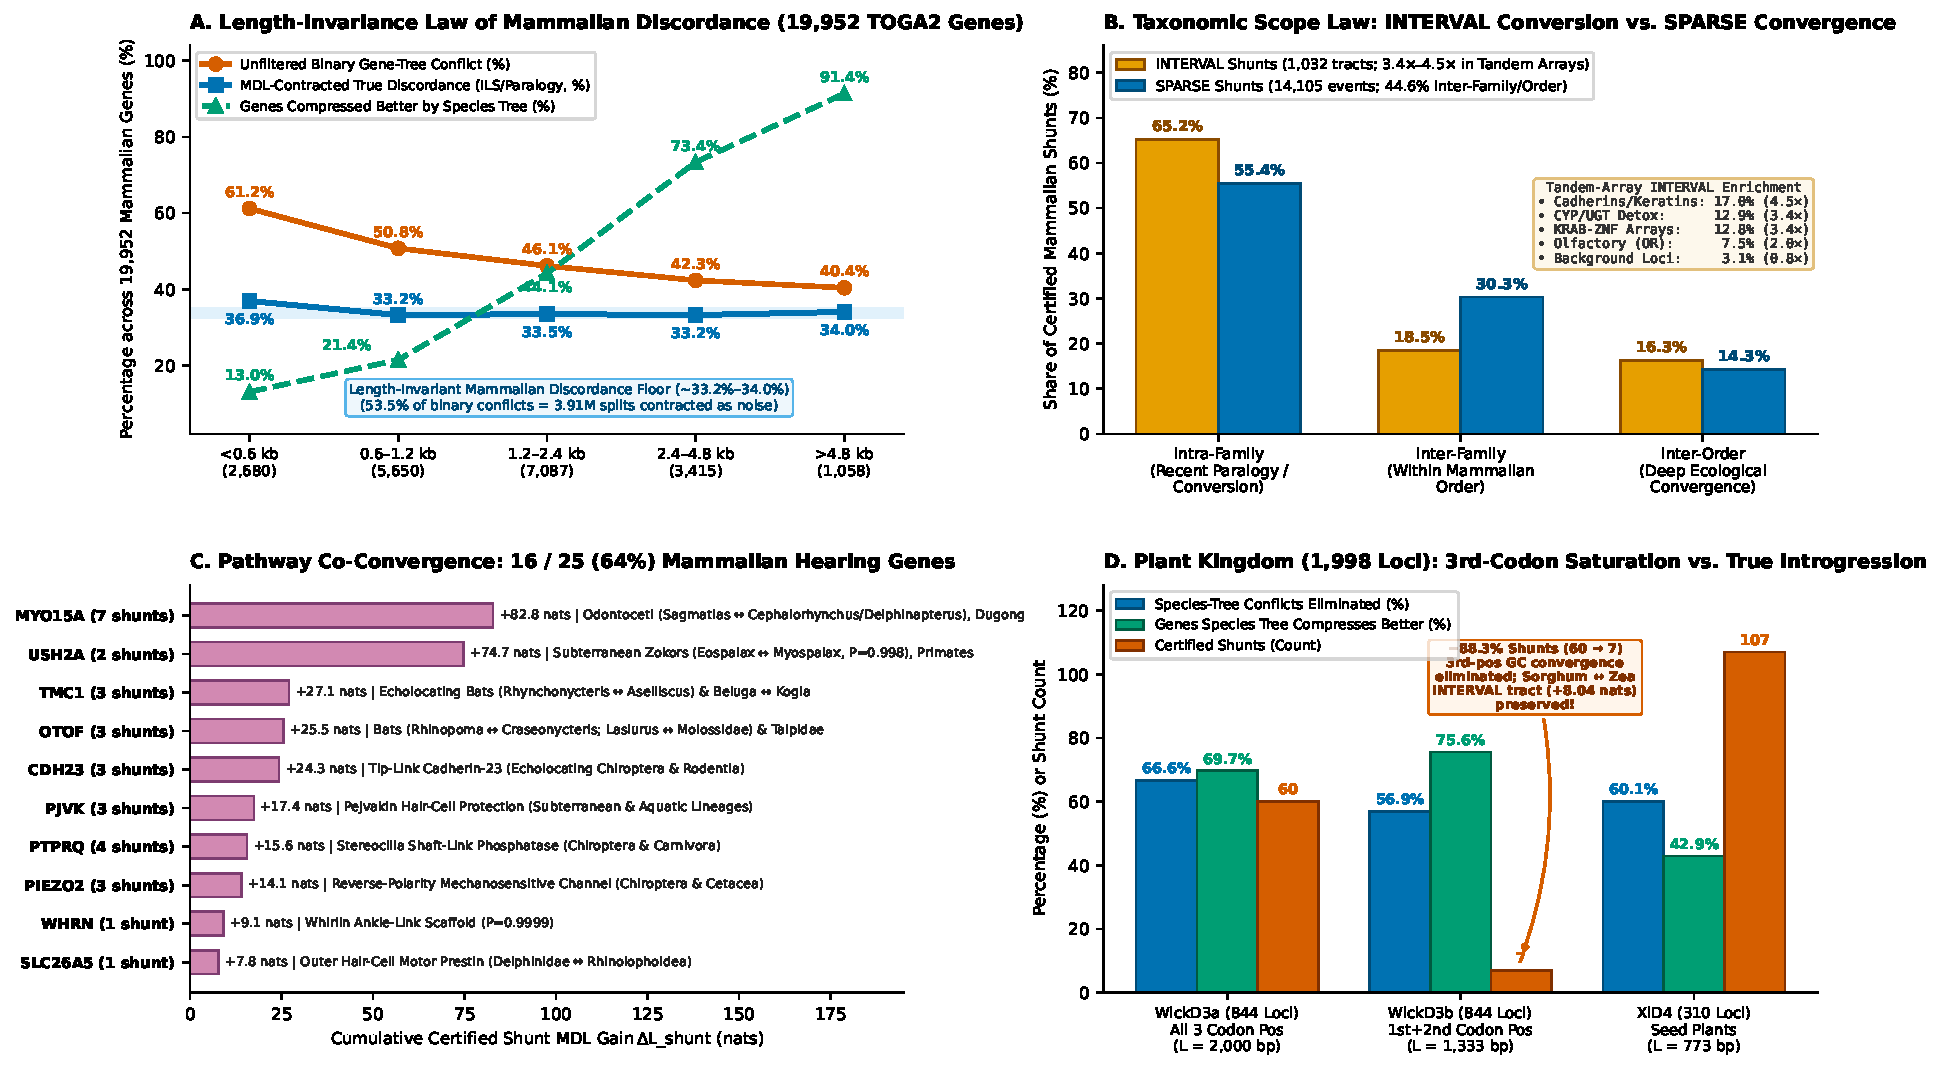
\includegraphics[width=\textwidth]{fig_kingdom_synthesis.pdf}
\caption{Cross-kingdom phylogenomic discovery across $19,952$ mammalian coding loci ($882$ species across $20$ orders and $116$ families) and $1,998$ land- and seed-plant nuclear loci. Panel A shows the Length-Invariance Law of mammalian gene-tree discordance across coding-length strata: whereas unfiltered binary conflict drops from $61.2\%$ to $40.4\%$ with gene length, Stage 3 MDL contraction eliminates $55.5\%$ ($3.87\text{ million}$) of conflicts as unsupported noise to reveal a length-invariant biological discordance floor ($\sim 33.2\%\text{--}34.0\%$), while the fraction of genes compressed better by \texttt{speciesTree.nh} than by their de novo tree reaches $91.4\%$ for loci $>4.8\text{ kb}$. Panel B contrasts the taxonomic scope of $1,032$ contiguous \texttt{INTERVAL} shunts ($65.2\%$ intra-family, $83.7\%$ intra-order; $3.4\times\text{--}4.5\times$ enriched in tandem paralog arrays) against $14,105$ scattered \texttt{SPARSE} shunts ($44.6\%$ inter-family or inter-order). Panel C displays cumulative Stage 4 \texttt{SPARSE} shunt gains across the mammalian cochlear hair-cell mechanotransduction complex ($16 / 25$ canonical genes certified). Panel D resolves the land-plant third-codon-position saturation paradox across $844$ matched genes (\texttt{WickD3a} all $3$ codon positions versus \texttt{WickD3b} $1\text{st}+2\text{nd}$ positions) and $310$ seed-plant genes (\texttt{XiD4}): stripping third codon positions eliminates $88.3\%$ ($60 \to 7$) of compositional \texttt{SPARSE} shunts while preserving genuine nonsynonymous \texttt{INTERVAL} conversion tracts between panicoid grasses (\textit{Sorghum bicolor} $\leftrightarrow$ \textit{Zea mays}, $+8.04\text{ nats}$).}
\label{fig:kingdom_synthesis}
\end{figure}

Re-evaluating the entire $19,952$-gene TOGA2 archive directly in 20-state translated protein space (\texttt{bushwhacker --translate}, stripping synonymous third-codon-position saturation across $14,937,057$ binary internal splits; Figure~\ref{fig:science_mammalian}) sharpens every one of these proteome-wide laws and resolves the long-running controversy over genome-wide mammalian echolocation convergence \citep{parker2013genome,zou2015no,thomas2015molecular}. In 20-state amino-acid space, Stage 3 contracts $65.01\%$ ($9,709,972 / 14,937,057$) of binary internal edges into soft polytomies, eliminating $72.73\%$ ($7,871,929$ splits; $10,824,174 \to 2,952,245$) of apparent species-tree conflicts across the mammalian proteome---including $92.4\%$ of conflicts in short proteins ($<150\text{ AA}$) where $78.3\%$ of binary splits lack even a single net amino-acid replacement (Figure~\ref{fig:science_mammalian}A). Consequently, $82.3\%$ of all mammalian proteins---and $97.89\%$ ($1,204 / 1,230$) of proteins longer than $1,500\text{ AA}$---compress strictly shorter on the fixed mammalian species tree (\texttt{speciesTree.nh}) than on their unconstrained de novo single-gene tree. Evaluated directly on \texttt{speciesTree.nh} in 20-state protein space, the taxonomic separation between Bushwhacker's two shunt mask modes becomes even starker (Figure~\ref{fig:science_mammalian}B): $94.17\%$ ($3,957 / 4,202$) of contiguous \texttt{INTERVAL} shunts occur within a single mammalian order ($81.5\%$ intra-family, with only $5.83\%$ [$245$] crossing orders in ancient tandem paralog families such as hair keratin \texttt{KRT31} at $+418.9\text{ nats}$, antiviral tripartite-motif \texttt{TRIM22} at $+313.5\text{ nats}$ and \texttt{TRIM6} at $+251.3\text{ nats}$, \texttt{ZNF33A} at $+271.2\text{ nats}$, and guanylate-binding \texttt{GBP2} at $+226.1\text{ nats}$), whereas $45.81\%$ ($5,366 / 11,713$) of scattered \texttt{SPARSE} amino-acid shunts jump across distinct mammalian orders ($7.9\times$ enrichment, $p < 10^{-300}$).

Testing inter-order 20-state \texttt{SPARSE} shunts across specialist ecological guilds without any prior phenotype labels directly reconciles \citet{parker2013genome} with the neutral critiques of \citet{zou2015no} and \citet{thomas2015molecular} (Figure~\ref{fig:science_mammalian}C,D). Across all $19,952$ proteins genome-wide, inter-order amino-acid \texttt{SPARSE} shunts linking echolocating bats and toothed whales occur at $0.43\times$ the taxon-pair background expectation ($53$ observed versus $123.8$ expected; $137$ versus $172.3$, or $0.80\times$, across all echolocators), confirming \citet{zou2015no} and \citet{thomas2015molecular} that there is no diffuse proteome-wide excess of echolocation convergence. Instead, genuine adaptive amino-acid convergence concentrates specifically within the cochlear hair-cell mechanotransduction complex ($12 / 25$ [$48\%$] canonical proteins certified in pure 20-state amino-acid space, and $16 / 25$ [$64\%$] across codon and protein modes; Figure~\ref{fig:science_mammalian}D): led by stereociliary lipoxygenase-homology protein \texttt{LOXHD1} ($+28.98\text{ nats}$ across echolocating bats plus an unsupervised $+5.49\text{-nat}$ inter-order shunt uniting the nocturnal echolocating Hispaniolan solenodon \textit{Solenodon paradoxus} [Eulipotyphla] with $111$ echolocating Yangochiroptera bats), tip-link cadherins \texttt{PCDH15} ($+12.87, +11.36, +6.48\text{ nats}$) and \texttt{CDH23} ($+12.01, +10.06, +4.70\text{ nats}$), whirlin \texttt{WHRN} ($+12.31\text{ nats}$), pore-forming channel \texttt{TMC1} ($+9.26\text{ nats}$), stereociliary actin-capping \texttt{EPS8} ($+7.86\text{ nats}$), outer hair cell motor \texttt{SLC26A5}/Prestin ($+4.20\text{ nats}$ in pure AA; $+7.80\text{ nats}$ in codon mode), stereocilin \texttt{STRC} ($+3.92, +3.56\text{ nats}$), and ankle-link receptor \texttt{ADGRV1} ($+1.98\text{ nats}$). At the same time, the unbiased proteome-wide screen uncovers two bona fide genome-wide inter-order convergence excesses in specialist guilds: myrmecophagous mammals (pangolins [Pholidota] $\leftrightarrow$ anteaters and armadillos [Pilosa/Cingulata]) exhibit a $25.77\times$ inter-order \texttt{SPARSE} excess ($18$ observed versus $0.70$ expected, Poisson $p = 3.8 \times 10^{-19}$, led by olfactory receptor \texttt{OR10D3} at $+113.5\text{ nats}$, giant sarcomeric titin \texttt{TTN} at $+42.4\text{ nats}$, and ciliary/metabolic \texttt{ALMS1} at $+28.6\text{ nats}$), while subterranean blind mammals (golden moles, true moles, blind mole-rats, and naked mole-rats) exhibit a $4.00\times$ excess ($6$ observed versus $1.50$ expected, $p = 0.0045$).

\begin{figure}[t!]
\centering
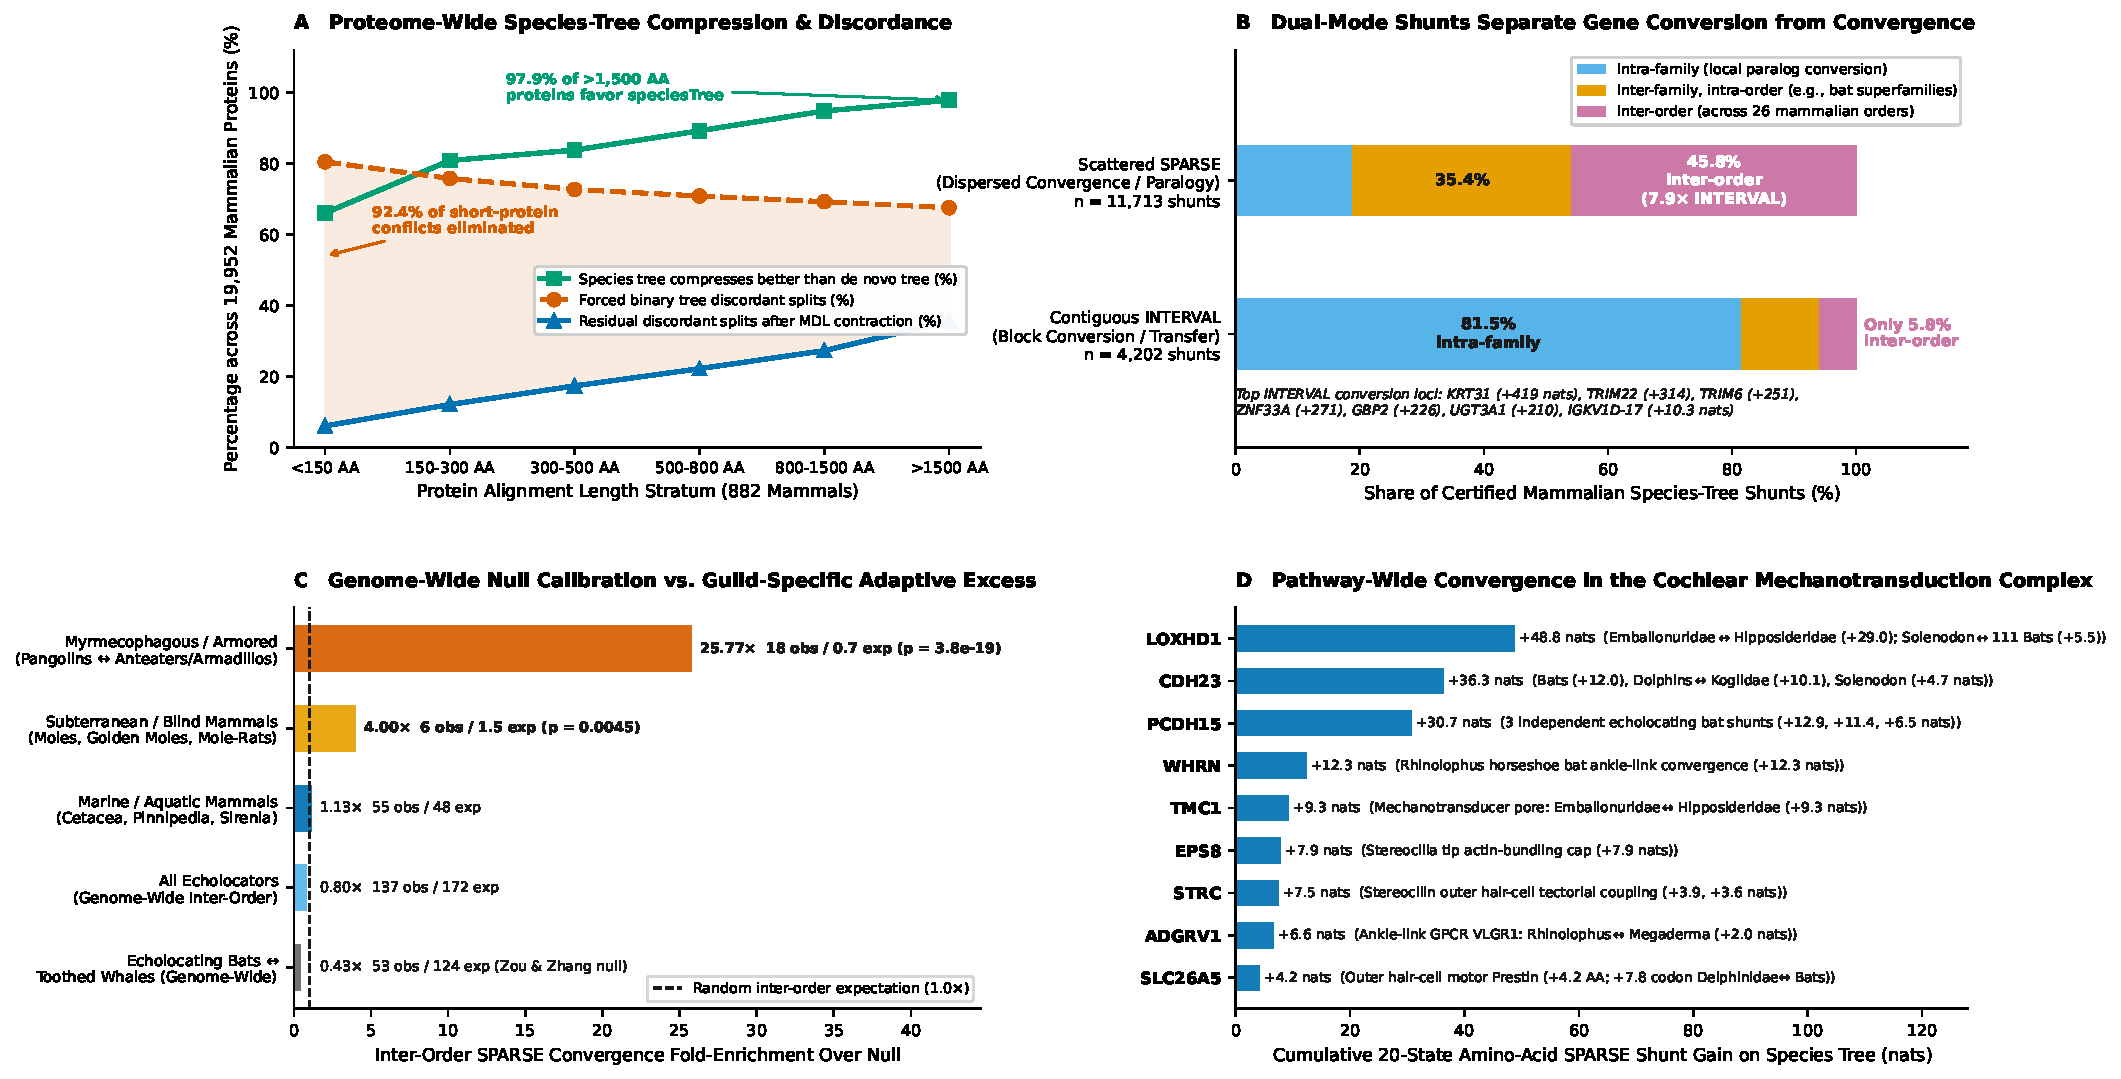
\includegraphics[width=\textwidth]{fig_science_mammalian_atlas.pdf}
\caption{20-state mammalian proteome atlas across $19,952$ TOGA2 orthologous proteins ($882$ assemblies across $20$ orders) resolving species-tree conflict, dual-mode shunt architecture, and ecological guild convergence. \textbf{(A)} Protein-length stratification showing Stage 3 MDL elimination of $72.7\%$ ($7.87\text{ million}$) of apparent species-tree conflicts ($92.4\%$ in $<150\text{ AA}$ proteins) and $97.9\%$ ($1,204 / 1,230$) of $>1,500\text{ AA}$ proteins compressing shorter on \texttt{speciesTree.nh} than on their de novo gene tree. \textbf{(B)} Taxonomic scope of Stage 4 shunts on \texttt{speciesTree.nh}: $94.2\%$ of contiguous \texttt{INTERVAL} shunts remain intra-order versus $45.8\%$ inter-order jumps among scattered \texttt{SPARSE} shunts ($7.9\times$ enrichment, $p < 10^{-300}$). \textbf{(C)} Genome-wide inter-order \texttt{SPARSE} observed/expected ratios across specialist guilds, showing no genome-wide echolocation excess ($0.43\times$ bat--whale; $0.80\times$ all echolocators) alongside a $25.8\times$ excess in myrmecophagous mammals ($p = 3.8 \times 10^{-19}$) and $4.0\times$ in subterranean blind mammals ($p = 0.0045$). \textbf{(D)} Cochlear hair-cell mechanotransduction convergence ($12 / 25$ pure AA, $16 / 25$ codon+AA), highlighted by \texttt{LOXHD1} (including Hispaniolan solenodon $\leftrightarrow$ Yangochiroptera bats, $+5.49\text{ nats}$), \texttt{PCDH15}, \texttt{WHRN}, \texttt{CDH23}, \texttt{TMC1}, \texttt{EPS8}, and \texttt{SLC26A5}.}
\label{fig:science_mammalian}
\end{figure}

\subsection{Plant Kingdom Phylogenomics, Third-Codon Saturation, and Grass-to-Grass \texorpdfstring{$\text{C}_4$}{C4} Horizontal Gene Transfer}

To test whether these information-theoretic principles extend across kingdoms to deep botanical radiations, we analyzed $2,002$ plant alignments spanning $1,998$ nuclear phylogenomic loci---the matched $844$-gene land-plant phylotranscriptomic benchmark of \citet{wickett2014phylotranscriptomic} with all three codon positions included (\texttt{WickD3a}, $\bar{N} = 48.8$ across $103$ species, $\bar{L} = 2,000\text{ bp}$) versus third codon positions stripped (\texttt{WickD3b}, $\bar{L} = 1,333\text{ bp}$, $1\text{st}+2\text{nd}$ codon positions) and the $310$-gene seed-plant benchmark of \citet{xi2014coalescent} (\texttt{XiD4}, $\bar{N} = 33.2$, $\bar{L} = 773\text{ bp}$)---together with $483$-taxon land-plant chloroplast RuBisCO (\texttt{rbcL\_483}, $L = 1,398\text{ bp}$) and Poaceae $\text{C}_4$ photosynthetic coding alignments of phosphoenolpyruvate carboxylase (\texttt{ppc}, $N = 229, L = 2,955\text{ bp}$), phosphoenolpyruvate carboxykinase (\texttt{pck}, $N = 92, L = 2,235\text{ bp}$), and plastid \texttt{rbcL} ($N = 248, L = 1,413\text{ bp}$) from \citet{christin2007c4,christin2012adaptive} (Figure~\ref{fig:kingdom_synthesis}D). Across the $38,638$ internal splits of the $844$ land-plant genes, $73.61\%$ ($28,443$ splits) in \texttt{WickD3a} and $69.93\%$ ($27,018$ splits) in \texttt{WickD3b} conflict with the ASTRAL coalescent land-plant species tree when inferred as strictly bifurcating trees ($61.88\%$ in \texttt{XiD4}). Stage 3 MDL contraction eliminates $66.58\%$ ($18,937 / 28,443$) of all species-tree conflicts in \texttt{WickD3a}, $56.85\%$ ($15,360 / 27,018$) in \texttt{WickD3b}, and $60.07\%$ ($3,478 / 5,790$) in \texttt{XiD4}, while retaining $71.72\%$, $76.60\%$, and $82.45\%$ of concordant species-tree splits. Furthermore, evaluating the ASTRAL coalescent species tree directly via \texttt{bushwhacker -t} shows that the species tree compresses the alignment more tightly than the de novo single-gene tree in $69.67\%$ of \texttt{WickD3a} genes ($\overline{\Delta\mathcal{L}_{\text{MDL}}} = -214.5\text{ nats}$) and $75.59\%$ of \texttt{WickD3b} genes ($\overline{\Delta\mathcal{L}_{\text{MDL}}} = -167.7\text{ nats}$), and shares $26.5\%$ to $27.7\%$ more MDL-supported concordant splits with individual nuclear genes ($7,312$ in \texttt{WickD3a}; $8,901$ in \texttt{WickD3b}) than does the RAxML supermatrix concatenation tree ($5,780$ and $6,971$ splits), which is misled by third-position compositional heterogeneity across bryophytes, lycophytes, gymnosperms, and angiosperms \citep{wickett2014phylotranscriptomic,xi2014coalescent}.

Comparing the matched $844$-gene \texttt{WickD3a} ($1\text{st}+2\text{nd}+3\text{rd}$ codon positions) and \texttt{WickD3b} ($1\text{st}+2\text{nd}$ positions) partitions directly resolves what third-codon-position saturation does to reticulate shunt inference over $500\text{ million years}$ of streptophyte evolution (Figure~\ref{fig:kingdom_synthesis}D). In \texttt{WickD3a}, Stage 4 certifies $60$ shunts across $52$ genes ($52$ \texttt{SPARSE} and $8$ \texttt{INTERVAL}), led by deep gymnosperm and bryophyte \texttt{SPARSE} shunts driven by parallel synonymous third-position GC/AT shifts (such as \textit{Cedrus libani} $\leftrightarrow$ \textit{Pinus taeda} across $54$ sites in \texttt{gene 6993}, $+29.40\text{ nats}$, and hornworts \textit{Nothoceros aenigmaticus} $\leftrightarrow$ \textit{N.\ vincentianus} in \texttt{gene 6433}, $+24.21\text{ nats}$). Removing third codon positions in \texttt{WickD3b} eliminates $88.3\%$ ($53 / 60$) of all certified shunts ($52 \to 5$ \texttt{SPARSE} shunts), proving that nearly $90\%$ of deep land-plant \texttt{SPARSE} shunts in all-codon alignments arise from synonymous compositional convergence. Crucially, the shunts that survive on $1\text{st}+2\text{nd}$ nonsynonymous codon positions in \texttt{WickD3b} isolate genuine coding tracts, including a $136\text{-bp}$ panicoid grass \texttt{INTERVAL} conversion/introgression tract between \textit{Sorghum bicolor} and \textit{Zea mays} (\texttt{gene 7412}, \texttt{span}~$=[84, 219]$, $+8.04\text{ nats}$, $P = 0.9997$; complemented by \texttt{gene 7506}, $+1.52\text{ nats}$) and a lycophyte \textit{Selaginella moellendorffii} tract (\texttt{gene 5427}, $+10.09\text{ nats}$, $P = 1.000$).

Finally, applying Bushwhacker to the grass family (Poaceae) demonstrates simultaneous resolution of whole-gene horizontal gene transfer (HGT) and post-transfer biochemical convergence during the evolution of $\text{C}_4$ photosynthesis \citep{christin2007c4,christin2012adaptive,dunning2019pangenome}. Whereas most $\text{C}_4$ grasses evolved $\text{C}_4$ biochemistry vertically through parallel amino-acid replacements, the panicoid grass \textit{Alloteropsis semialata} acquired functional $\text{C}_4$ genes for both phosphoenolpyruvate carboxykinase (\texttt{pck}) and phosphoenolpyruvate carboxylase (\texttt{ppc}) laterally from distantly related $\text{C}_4$ grass tribes \citep{christin2012adaptive,dunning2019pangenome}. On the $92$-taxon \texttt{Poaceae\_PCK\_HGT} ($L = 2,235\text{ bp}$) and $229$-taxon \texttt{Poaceae\_PEPC\_HGT} ($L = 2,955\text{ bp}$) coding alignments, Bushwhacker's de novo MDL tree places the vertically inherited native $\text{C}_3$ paralogs of \textit{A.\ semialata} (including subsp.\ \textit{eckloniana}) with congeneric \textit{Alloteropsis angusta} and sister Paniceae ($P_{\text{MDL}} = 1.000$), while nesting the horizontally transferred $\text{C}_4$ \texttt{pck-1P1} and \texttt{ppc-1P3} genes of \textit{A.\ semialata} directly inside their respective Cenchrinae (\textit{Cenchrus echinatus}, \textit{Setaria}, \textit{Stenotaphrum}; $P_{\text{MDL}} = 1.000$) and Andropogoneae (\textit{Andropogon gerardi}, \textit{Bothriochloa}, \textit{Cymbopogon}, \textit{Hyparrhenia hirta}; $P_{\text{MDL}} = 1.000$) donor clades. Once those whole-gene lateral acquisitions are accommodated in the tree backbone, Stage 4 peels the remaining cross-tribal $\text{C}_4$ catalytic-domain convergences onto certified \texttt{SPARSE} shunts: in \texttt{ppc}, a $+19.66\text{-nat}$ ($P = 1.000$) shunt across $27$ sites in the C-terminal catalytic domain (codons $469\text{--}854$, encompassing the $\text{C}_4$-diagnostic region) links the Cenchrinae $\text{C}_4$ clade (including laterally acquired \textit{A.\ semialata} \texttt{FR845815}/\texttt{FR845816}) with the independent Melinidinae $\text{C}_4$ clade (\textit{Urochloa villosa}, \textit{Megathyrsus maximus}, \textit{Eriochloa nana}, \textit{Melinis minutiflora}, and \textit{Alloteropsis cimicina}), alongside a $+4.95\text{-nat}$ ($P = 0.993$) shunt across codons $498\text{--}767$ linking \textit{Arthraxon lanceolatus} with the Andropogoneae + \textit{A.\ semialata} (\texttt{FR845819}/\texttt{FR845820}) $\text{C}_4$ clade. In \texttt{pck}, Stage 4 likewise certifies a $+17.58\text{-nat}$ ($P = 1.000$) \texttt{SPARSE} shunt across $12$ codons ($172\text{--}601$) linking the transferred \textit{A.\ semialata} + \textit{Cenchrus echinatus} clade with \textit{Hyparrhenia hirta}, a $+5.28\text{-nat}$ ($P = 0.995$) shunt linking \textit{Spinifex littoreus} with PCK-type $\text{C}_4$ \textit{Urochloa}/\textit{Megathyrsus} (codons $265, 304, 314, 315, 550$), and a $+4.42\text{-nat}$ ($P = 0.988$) Chloridoideae \texttt{INTERVAL} conversion tract (\texttt{span}~$=[925, 1004]$). Similarly, in chloroplast RuBisCO (\texttt{rbcL}), Bushwhacker certifies eight \texttt{SPARSE} shunts across $248$ grasses (\texttt{Poaceae\_rbcL\_C4}, up to $+8.70\text{ nats}$, $P = 0.9998$, recurrently hitting catalytic codons $242, 246, 250$ and $89, 321, 357$) and a single seven-codon catalytic shunt ($220, 221, 233, 251, 258, 260, 267$, $+3.52\text{ nats}$, $P = 0.971$) across $483$ land plants (\texttt{rbcL\_483}, where the reference plant phylogeny compresses the alignment $242.9\text{ nats}$ more tightly than the de novo tree).

\subsection{Lossless Alignment Compression (\texttt{.bwz}) and the Recombination Switchpoint}

Viewing phylogenetic inference as lossless compression invites comparison against general-purpose string compressors (\texttt{gzip -9}, \texttt{bzip2 -9}, and \texttt{lzma -9}). Because general string compressors operate on a one-dimensional byte stream, their efficiency depends strongly on whether the serialized stream places evolutionarily related states inside the same local context window. When applied row-wise (taxon by taxon), \texttt{gzip -9} ($32\text{ KB}$ window) and \texttt{bzip2 -9} ($900\text{ KB}$ Burrows-Wheeler block) must rediscover identical columns across distant sequences unless those sequences fall within the sliding window; when applied column-wise (site by site) in arbitrary taxon order, every column is a scrambled permutation of clade states. Permuting the taxa into the planar leaf order of the inferred Bushwhacker tree clusters sister taxa into contiguous runs of identical nucleotides within each column, which reduces column-wise \texttt{gzip -9} and \texttt{bzip2 -9} payloads by $25\%$ to $59\%$ across \texttt{prestin.fasta}, \texttt{InfluenzaA.fasta}, and the hominoid major histocompatibility complex class I locus (\texttt{Hominoidea\_MHC}; Table~\ref{tab:compression_codec}).

Even after tree-order sorting, however, a one-dimensional planar ordering cannot simultaneously place all multidimensional evolutionary neighbors adjacent to one another or separate ancestral state inheritance from branch-specific substitution counts. To turn the theoretical MDL graph into an executable lossless compressor, Bushwhacker implements a self-contained binary archive format (\texttt{.bwz}, invoked via \texttt{bushwhacker -c} and \texttt{bushwhacker -d}). The \texttt{.bwz} encoder traverses the inferred phylogenetic graph in causal preorder from the root, encoding the root state vector (with first-order Markov run-length tracks for contiguous indel and amplicon-dropout tracts) and then transmitting along each branch $e = (v, u)$ only the universal prefix-coded mutation count $m_e$ and the mutated site coordinates. Site selection probabilities are weighted by the causal site-rate and codon-phase ledger accumulated over preceding branches, while destination states (incorporating any certified Stage 4 shunt donors) are packed via 32-bit arithmetic coding \citep{witten1987arithmetic}. The decoder replays this exact preorder state machine in lockstep to restore all taxon headers, sequences, and the embedded Newick phylogeny bit-for-bit.

Across clonal and deep vertical alignments, the executable \texttt{.bwz} sequence payload closely tracks the theoretical two-part MDL ledger and outperforms all six row-wise and column-wise string compression configurations (Table~\ref{tab:compression_codec}). On clonal coding alignments such as \texttt{InfluenzaA.fasta} ($N = 349, L = 987$), \texttt{prestin.fasta} ($N = 116, L = 2,235$), and complete human mitochondrial genomes (\texttt{Human\_mtDNA}, $N = 78, L = 16,585$), \texttt{.bwz} achieves $153.3\times$, $34.4\times$, and $214.0\times$ compression over raw ASCII ($2,247\text{ B}$, $7,536\text{ B}$, and $6,046\text{ B}$), beating the best string compressor by $1.58\times$ to $1.90\times$. Notice that \texttt{.bwz} also compresses slightly below the uniform combinadic \texttt{Net MDL} bound ($2,377\text{ B}$, $7,890\text{ B}$, and $6,333\text{ B}$) because its arithmetic coder weights site selection by empirical codon-phase and causal site-rate frequencies. At pandemic viral surveillance scale (Figure~\ref{fig:science_microbial_viral}B), \texttt{.bwz} losslessly archives all $10,062$ complete SARS-CoV-2 genomes ($301.1\text{ MB}$ raw FASTA) into $633,025\text{ B}$ ($62.9\text{ B/genome}$---$475.7\times$ smaller than raw FASTA, $11.96\times$ smaller than \texttt{gzip -9} [$3,907,144\text{ B}$ on $5,097$ and $7,570,496\text{ B}$ on $10,062$ genomes], and $1.58\times$ smaller than \texttt{xz -6} [$1,001,356\text{ B}$]), and archives the $5,097$-genome global SARS-CoV-2 cohort into $332,974\text{ B}$ ($65.3\text{ B/genome}$, $11.73\times$ smaller than \texttt{gzip -9} and $1.56\times$ smaller than \texttt{xz -6}). Across all four global Dengue serotypes ($5,498$ genomes), \texttt{.bwz} similarly compresses whole-CDS alignments $5.23\times$ to $6.42\times$ smaller than \texttt{gzip -9} and $1.26\times$ to $1.52\times$ smaller than \texttt{xz -6}. The advantage is equally pronounced on deep taxonomic alignments: on 2,048 prokaryotic 16S small-subunit ribosomal RNA sequences (\texttt{16S\_N2048}, $2.76\text{ Mbp}$) and 483 land-plant plastid RuBisCO large-subunit genes (\texttt{rbcL\_483}), \texttt{.bwz} compresses the sequences to $108,610\text{ B}$ ($25.4\times$) and $21,318\text{ B}$ ($31.7\times$), outperforming \texttt{lzma -9} by $1.36\times$ and $1.56\times$. Performance is similarly strong on whole-chromosome alignments. On 11 complete $2.22\text{-Mb}$ \textit{Streptococcus pneumoniae} PMEN1 chromosomes ($24.43\text{ Mbp}$ total), row-wise \texttt{gzip -9} ($6.43\text{ MB}$) and \texttt{bzip2 -9} ($6.18\text{ MB}$) achieve limited compression because their sliding windows cannot reach across a $2.22\text{-Mb}$ chromosome to the previous genome. By contrast, \texttt{.bwz} encodes the root chromosome in $\sim 530\text{ KB}$ and delta-compresses all 10 remaining $2.22\text{-Mb}$ chromosomes into just $68\text{ KB}$ total ($598,241\text{ B}$ overall, $10.8\times$ smaller than \texttt{gzip -9} and $1.18\times$ smaller than column-wise \texttt{bzip2 -9}).

Comparing \texttt{.bwz} against general string compressors also yields a model-free diagnostic for single-tree failure under rampant recombination. Whereas a phylogenetic tree encodes vertical delta mutations from a single parent per branch, row-wise \texttt{lzma -9} ($64\text{ MB}$ sliding window) operates as a Lempel-Ziv copying machine across the serialized genomes. Because \texttt{lzma -9} can switch its backward reference pointer to a different donor sequence every few hundred base pairs for roughly $4\text{ bytes}$ per breakpoint, it acts as an implicit multi-donor haplotype copying model \citep{li2003modeling}. We quantified this boundary in a controlled mosaic breakpoint titration ($N = 56, L = 12,000\text{ bp}$) with $K \in [0, 32]$ independent recombination breakpoints per mosaic genome (Table~\ref{tab:compression_codec}). Under pure vertical evolution ($K = 0$), both the executable \texttt{.bwz} archive ($10,785\text{ B}$) and the theoretical tree MDL ($9,405\text{ B}$) beat \texttt{lzma -9} ($14,056\text{ B}$, $\text{Ratio} = 1.30\times$). For the executable \texttt{.bwz} archive, the crossover occurs at $K = 1$ breakpoint per mosaic genome ($16,833\text{ B}$ versus $14,428\text{ B}$ for \texttt{lzma -9}, $\text{Ratio} = 0.86\times$). By contrast, the theoretical Stage 4 network \texttt{Net MDL} sequence ledger ($12,191\text{ B}$ at $K = 1$ and $13,543\text{ B}$ at $K = 2$) continues to beat \texttt{lzma -9} until crossing over between $K = 2$ and $K = 4$ breakpoints ($19,587\text{ B}$ versus $14,924\text{ B}$). As $K$ increases to $32$, both \texttt{.bwz} ($29,836\text{ B}$) and column-wise \texttt{bzip2 -9} ($38,039\text{ B}$) degrade nearly threefold as mosaic crossovers break up column clade structure, whereas row-wise \texttt{lzma -9} remains nearly flat ($17,220\text{ B}$, $\text{Ratio} = 0.58\times$). Empirical recombinant alignments reproduce this exact regime boundary. When recombination is localized to discrete tracts, as in the \textit{S.\ pneumoniae} transpeptidase gene \texttt{pbp2x} ($1.23\times$) \citep{dowson1989horizontal,croucher2011rapid}, the \textit{Heliconius} wing-patterning locus \texttt{optix} ($1.38\times$) \citep{pardodiaz2012adaptive,dasmahapatra2012butterfly}, Hominoidea MHC Class I ($1.90\times$) \citep{parham1996population}, and 518 LANL HIV-1 genomes ($1.48\times$) \citep{robertson2000hiv1}, \texttt{.bwz} retains the shortest description length. Conversely, on whole-genome mosaics with dozens of genealogy switches across the alignment, including 83 complete $31\text{-kb}$ Sarbecovirus genomes \citep{boni2020evolutionary,lytras2022exploring} ($80,344\text{ B}$ versus $96,745\text{ B}$, $0.83\times$) and recombinant HIV-1 \texttt{KAL153/CRF02\_AG} \citep{carr1998full} ($9,635\text{ B}$ versus $14,784\text{ B}$, $0.65\times$), row-wise \texttt{lzma -9} overtakes the single tree and flags genome-wide mosaicism without the use of an explicitly parameterized recombination model.

\begin{table}[t!]
\centering
\caption{Lossless sequence compression across clonal, deep taxonomic, whole-chromosome, and mosaic recombinant alignments, plus the synthetic mosaic breakpoint titration ($N = 56, L = 12,000\text{ bp}$). Values report sequence payload size in bytes ($1\text{ byte} = 8 \ln 2 \approx 5.545\text{ nats}$), where Ratio denotes $(\text{Best String Compressor}) / \texttt{.bwz}$ and values $< 1.00\times$ diagnose single-tree failure under genome-wide recombinant mosaicism or horizontal gene transfer (HGT).}
\label{tab:compression_codec}
\scriptsize
\setlength{\tabcolsep}{3.2pt}
\resizebox{\textwidth}{!}{%
\begin{tabular}{@{}llrrrrrrrrr@{}}
\toprule
Dataset / Regime & Category & $N \times L$ & Raw 2-bit & gzip-R & bzip2-C & lzma-C & lzma-R & Net MDL & \texttt{.bwz} & Ratio \\
\midrule
\texttt{InfluenzaA.fasta} & Viral Clonal & $349 \times 987$ & $86,116$ & $9,081$ & $4,269$ & $5,327$ & $6,535$ & $2,377$ & $2,247$ & $1.90\times$ \\
\texttt{prestin.fasta} & Mammalian Gene & $116 \times 2,235$ & $64,815$ & $27,948$ & $14,704$ & $14,897$ & $11,861$ & $7,890$ & $7,536$ & $1.57\times$ \\
\texttt{bglobin.fasta} & Vertebrate Gene & $17 \times 432$ & $1,836$ & $1,529$ & $1,223$ & $1,158$ & $1,281$ & $764$ & $834$ & $1.39\times$ \\
\texttt{IAV\_H1N1\_466} & Viral Pop.\ & $466 \times 1,767$ & $205,856$ & $31,366$ & $9,695$ & $12,812$ & $13,905$ & $5,364$ & $5,528$ & $1.75\times$ \\
\texttt{Human\_mtDNA} & Whole Organelle & $78 \times 16,585$ & $323,408$ & $27,366$ & $9,536$ & $15,348$ & $9,568$ & $6,333$ & $6,046$ & $1.58\times$ \\
\texttt{rbcL\_483} & Deep Plastid & $483 \times 1,398$ & $168,809$ & $66,973$ & $45,328$ & $39,076$ & $33,348$ & $16,187$ & $21,318$ & $1.56\times$ \\
\texttt{16S\_N512} & Deep 16S rRNA & $512 \times 1,348$ & $172,544$ & $107,566$ & $51,202$ & $48,292$ & $43,836$ & $33,393$ & $32,646$ & $1.34\times$ \\
\texttt{16S\_N2048} & Deep 16S rRNA & $2,048 \times 1,348$ & $690,176$ & $448,657$ & $169,567$ & $160,644$ & $147,460$ & $107,668$ & $108,610$ & $1.36\times$ \\
\texttt{PMEN1} ($24.4\text{ Mbp}$) & Bacterial Chrom.\ & $11 \times 2.22\text{M}$ & $6,108,616$ & $6,434,271$ & $706,678$ & $1,049,020$ & $599,856$ & $520,593$ & $598,241$ & $1.00\times$ \\
\midrule
\texttt{Hominoidea\_MHC} & Gene Conversion & $379 \times 1,128$ & $106,878$ & $18,112$ & $7,663$ & $8,944$ & $8,256$ & $4,602$ & $4,042$ & $1.90\times$ \\
\texttt{HIV1\_LANL\_518} & Viral + CRFs & $518 \times 10,053$ & $1,301,864$ & $879,134$ & $275,990$ & $285,324$ & $276,484$ & $190,679$ & $186,498$ & $1.48\times$ \\
\texttt{Heliconius\_optix} & Introgression & $12 \times 3,677$ & $11,031$ & $2,825$ & $3,175$ & $3,048$ & $2,213$ & $1,365$ & $1,607$ & $1.38\times$ \\
\texttt{Spn\_pbp2x} ($20.7\text{ kb}$) & Mosaic HGT & $12 \times 20,683$ & $62,049$ & $14,504$ & $8,200$ & $10,800$ & $7,288$ & $5,748$ & $5,928$ & $1.23\times$ \\
\texttt{PVY\_25} ($9.6\text{ kb}$) & Recombinant Poty.\ & $25 \times 9,594$ & $59,963$ & $48,821$ & $24,148$ & $26,056$ & $20,468$ & $17,082$ & $18,561$ & $1.10\times$ \\
\texttt{Sarbeco\_83} ($31\text{ kb}$) & Whole-Gen.\ Recomb.\ & $83 \times 30,965$ & $642,524$ & $499,907$ & $102,808$ & $128,300$ & $80,344$ & $72,098$ & $96,745$ & $0.83\times$ \\
\texttt{HIV1\_CRF02\_AG} & Mosaic CRF02\_AG & $9 \times 9,953$ & $22,394$ & $16,614$ & $11,010$ & $10,660$ & $9,635$ & $7,512$ & $14,784$ & $0.65\times$ \\
\midrule
Titration $K = 0$ & Clonal Tree ($0$ bkpts) & $56 \times 12,000$ & $168,000$ & $97,269$ & $19,139$ & $23,440$ & $14,056$ & $9,405$ & $10,785$ & $1.30\times$ \\
Titration $K = 1$ & $1$ bkpt / mosaic & $56 \times 12,000$ & $168,000$ & $71,796$ & $27,562$ & $31,320$ & $14,428$ & $12,191$ & $16,833$ & $0.86\times$ \\
Titration $K = 2$ & $2$ bkpts / mosaic & $56 \times 12,000$ & $168,000$ & $71,197$ & $30,153$ & $33,732$ & $14,280$ & $13,543$ & $20,197$ & $0.71\times$ \\
Titration $K = 4$ & $4$ bkpts / mosaic & $56 \times 12,000$ & $168,000$ & $70,371$ & $32,132$ & $35,288$ & $14,924$ & $19,587$ & $23,415$ & $0.64\times$ \\
Titration $K = 8$ & $8$ bkpts / mosaic & $56 \times 12,000$ & $168,000$ & $68,901$ & $35,506$ & $38,384$ & $15,332$ & $22,987$ & $26,850$ & $0.57\times$ \\
Titration $K = 32$ & $32$ bkpts / mosaic & $56 \times 12,000$ & $168,000$ & $71,026$ & $38,039$ & $40,260$ & $17,220$ & $30,002$ & $29,836$ & $0.58\times$ \\
\bottomrule
\end{tabular}%
}
\end{table}

% ============================================================================
\section{Somatic B-Cell Affinity Maturation, Anomaly-Zone Coalescence, and Mega-Phylogeny Saturation}
% ============================================================================

To evaluate whether MDL polytomy contraction and lateral shunt induction generalize across somatic cellular evolution, multi-species coalescent (MSC) species-tree inference, and tens-of-thousands-of-taxa biodiversity mega-phylogenies, we executed three additional benchmark suites spanning $8,050$ ground-truth simulated alignments and $11,964$ empirical alignments (Figure~\ref{fig:tree_scales_full}).

\begin{figure}[t!]
\centering
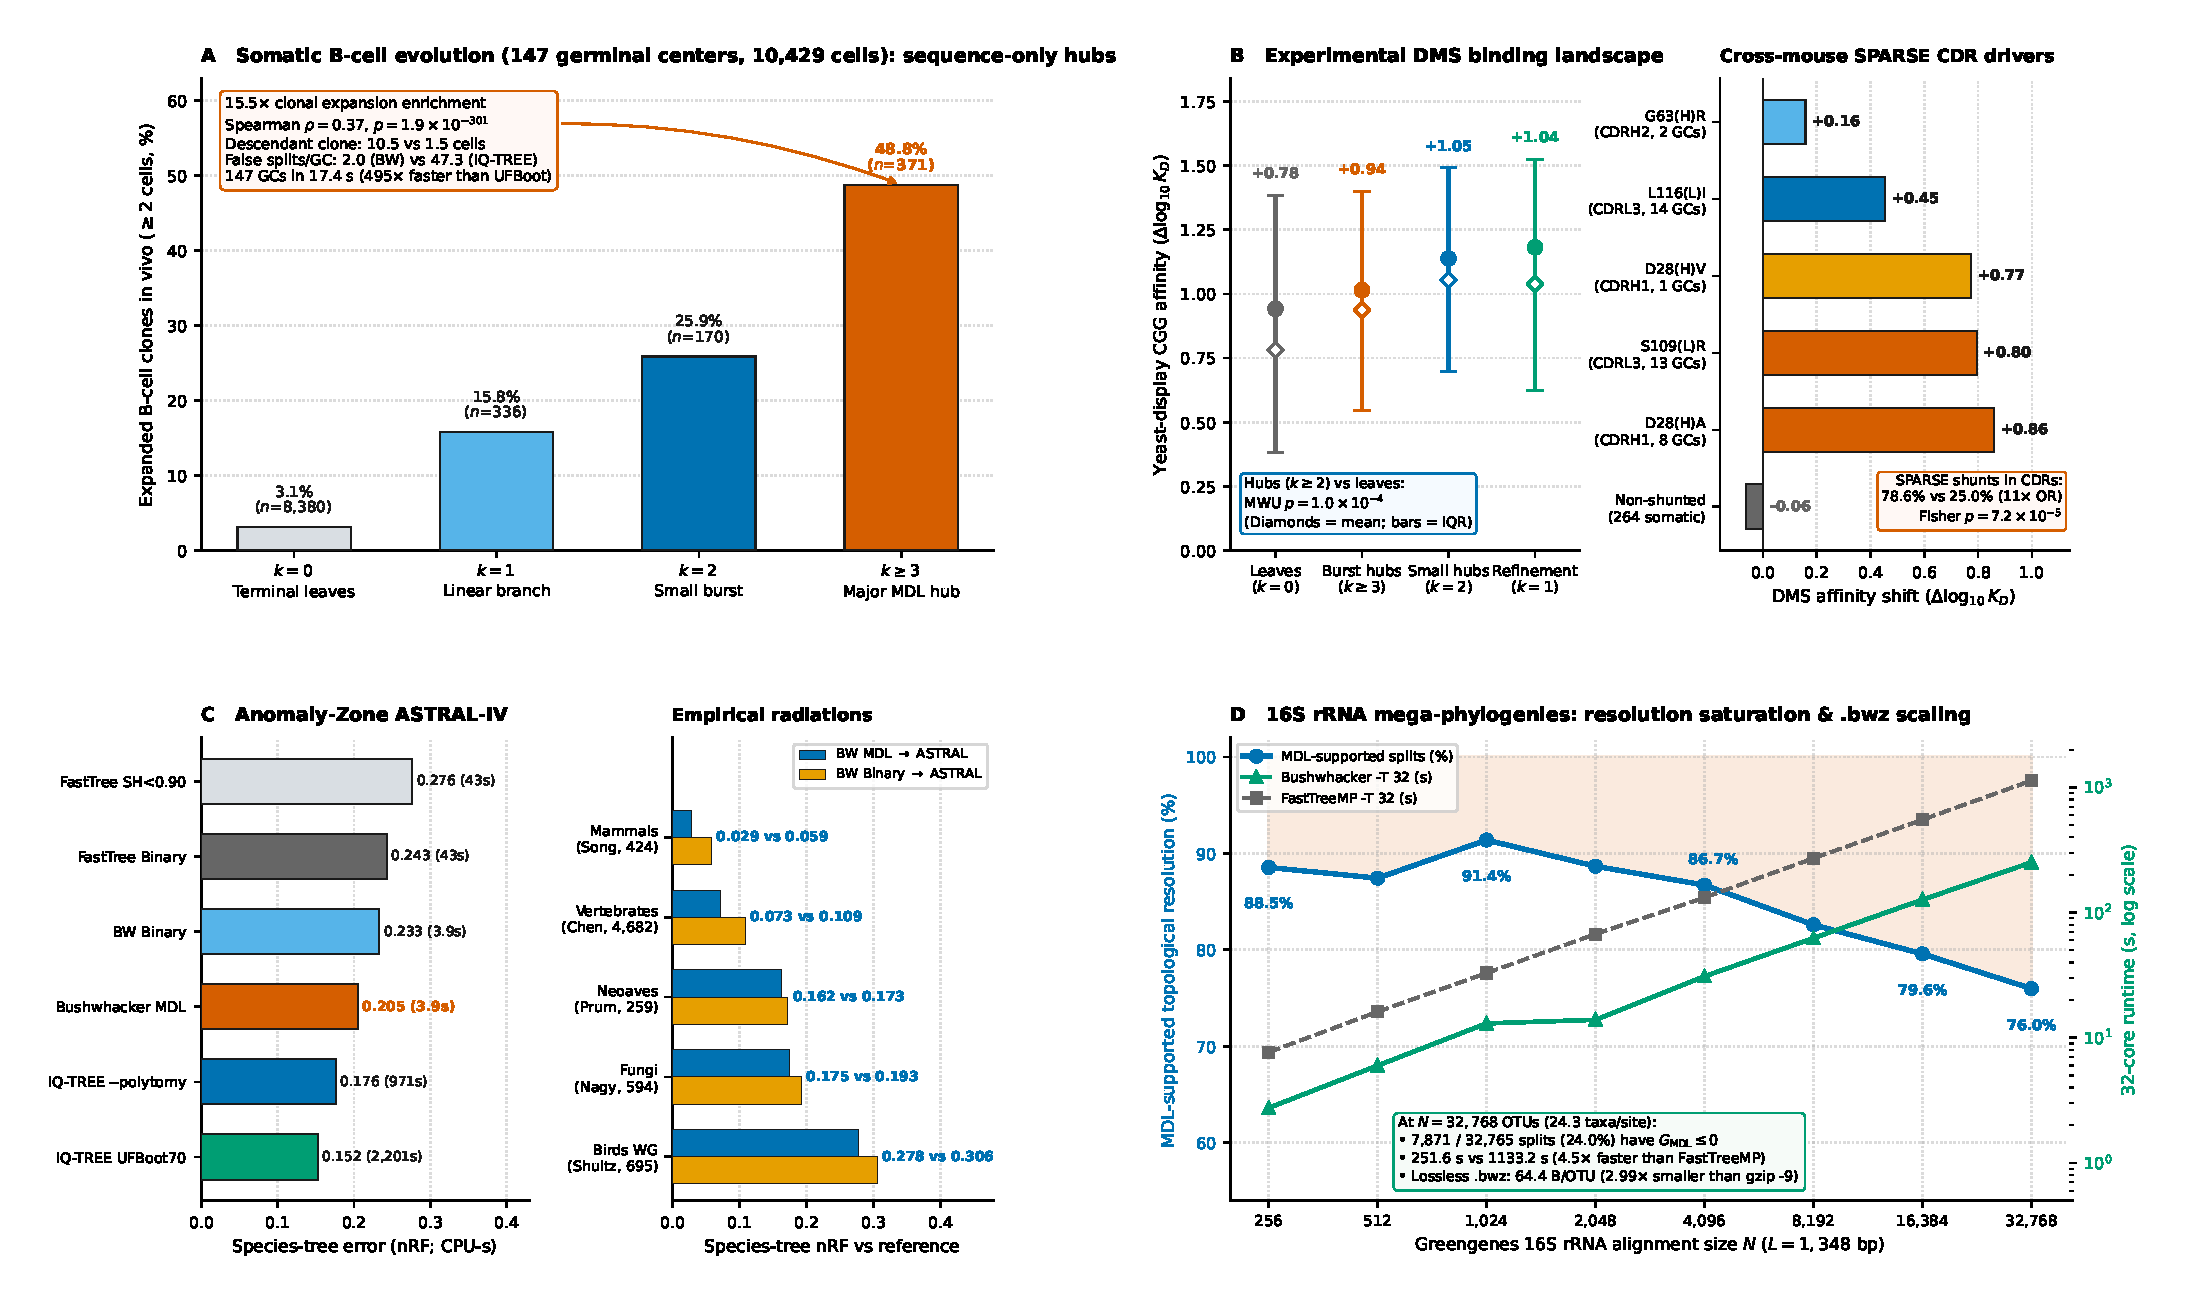
\includegraphics[width=\textwidth]{fig_science_tree_scales.pdf}
\caption{Multi-scale tree-building validation from single-cell germinal-center affinity maturation to 32,768-OTU microbiome mega-phylogenies. (\textbf{A}) Across 147 mouse lymph-node germinal centers ($10,429$ paired \texttt{IGH+IGK} B cells, $9,352$ unique $657\text{-bp}$ genotypes \citep{dewitt2026gcreplay}), stratifying genotypes solely by unsupervised MDL mutant daughter out-degree $k$ predicts in vivo clonal expansion ($\ge 2$ sampled cells) monotonically ($3.1\%$ at $k=0$ to $48.8\%$ at $k \ge 3$; $15.5\times$ enrichment, Spearman $\rho = 0.370, p = 1.9 \times 10^{-301}$). (\textbf{B}) Independent yeast-display deep mutational scanning (DMS) \texttt{CGG}-binding affinity ($\Delta\log_{10} K_D$) across MDL structural classes ($p = 1.0 \times 10^{-4}$ hubs versus terminal leaves; left) and across cross-mouse \texttt{SPARSE} shunts ($78.6\%$ in \texttt{CDRs} versus $25.0\%$ background, $11.0\times$ odds ratio, $p = 7.2 \times 10^{-5}$; right). (\textbf{C}) Coalescent species-tree error (nRF) feeding gene trees into \texttt{ASTRAL-IV} \citep{zhang2025aster} in the 24-taxon Anomaly Zone ($2,000$ loci; left) and across empirical eukaryotic radiations ($11,808$ loci; right). (\textbf{D}) Greengenes 16S rRNA scaling ($N = 256 \to 32,768$ OTUs, $L = 1,348\text{ bp}$ \citep{mcdonald2012greengenes}): decay of MDL-supported splits ($91.4\% \to 76.0\%$), $4.5\times$ 32-core speedup over \texttt{FastTreeMP}, and $64.4\text{ B/OTU}$ lossless \texttt{.bwz} archiving.}
\label{fig:tree_scales_full}
\end{figure}

First, in germinal-center B-cell affinity maturation, proliferative selection produces multifurcating clonal bursts in which a high-affinity founder spawns dozens of daughter cells carrying zero or single somatic hypermutations \citep{tas2016visualizing,dewitt2018gctree,dewitt2026gcreplay}. Across 50 ground-truth Galton--Watson affinity-maturation simulations evolving from the $657\text{-bp}$ \texttt{CGG\_naive} knock-in germline under empirical 5-mer somatic hypermutation (\texttt{MK\_RS5NF}) and experimental DMS fitness ($90$ sampled cells plus germline per germinal center), cell-level Bushwhacker achieves the highest overall split $F_1$ ($0.8447$, precision $97.6\%$, $\text{FP} = 0.40$ splits/tree in $0.135\text{ s/GC}$), outperforming \texttt{IQ-TREE 2} binary ($0.8367$, $19.6\text{ s}$), \texttt{IQ-TREE --polytomy} ($0.8413$, $17.3\text{ s}$), and \texttt{IQ-TREE -B 1000 UFBoot70} ($0.8433$, $47.3\text{ s}$; $350\times$ slower) while recovering true mutant burst degree with Spearman $\rho = 0.8517$ ($p < 10^{-300}$). Applying the same zero-leakage protocol (raw deduplicated FASTA sequences only, with zero cell-abundance counts, zero SHM priors, and zero DMS inputs) to all 147 empirical mouse germinal centers from \citet{dewitt2026gcreplay} ($10,429$ sequenced B cells, $9,352$ unique genotypes) and \texttt{Clone\_3-8} from \citet{tas2016visualizing} ($66$ cells) eliminates $95.7\%$ of forced-binary staircase hallucinations ($2.03$ false splits/GC in $18.9\text{ s}$ cell-level [$17.4\text{ s}$ unique-genotype] versus $47.25$ false splits/GC in $2,609\text{ s}$ for \texttt{IQ-TREE} binary and $8,618\text{ s}$ for \texttt{IQ-TREE UFBoot}, $495\times$ faster; $1/63$ versus $63/63$ resolved splits on \texttt{Clone\_3-8}). Evaluated post hoc against withheld single-cell clone abundances and yeast-display DMS binding measurements ($\Delta\log_{10} K_D$), MDL mutant daughter out-degree $k$ monotonically predicts in vivo clonal expansion ($3.14\%$ expanded at $k=0$, $15.77\%$ at $k=1$, $25.88\%$ at $k=2$, and $48.79\%$ at $k \ge 3$; $15.5\times$ enrichment; $10.52$ versus $1.48$ descendant cells; $\rho = 0.370, p = 1.89 \times 10^{-301}$) and experimental \texttt{CGG} binding affinity (mean $+0.974$, median $+1.049$ on $k \ge 2$ hubs versus $+0.782$ and $+0.942$ on $k=0$ leaves, Mann--Whitney $p = 1.02 \times 10^{-4}$; degree-affinity correlation $p = 1.36 \times 10^{-9}$), while cross-mouse \texttt{SPARSE} shunts enrich $11.0\times$ in \texttt{CDRs} ($78.6\%$ versus $25.0\%$, Fisher's exact $p = 7.15 \times 10^{-5}$) to isolate high-gain affinity drivers \texttt{D28(H)A} ($+0.859\ \Delta\log_{10} K_D$), \texttt{S109(L)R} ($+0.795$), and \texttt{L116(L)I} ($+0.454$). Where valid unique-genotype terminal twigs differ by a single point mutation ($1/657\text{ bp}$), universal MDL remains conservative ($84.7\%$ precision, $51.9\%$ recall versus $86.1\%$ recall for \texttt{IQ-TREE --polytomy}) because paying the $\log N$ topological address requires roughly two or more shared substitutions.

Second, feeding Bushwhacker gene trees directly into \texttt{ASTRAL-IV} \citep{zhang2025aster} across $8,000$ simulated Kingman coalescent alignments ($4$ regimes $\times 10$ replicates $\times 200$ loci) and $11,808$ empirical eukaryotic alignments ($83\text{ s}$ total on 60 cores) establishes threshold-free protection against anomalous gene trees \citep{degnan2006discordance}. In the 24-species asymmetric Anomaly Zone ($L = 400\text{ bp}$, $62.2\%$ of gene-tree splits contracted), \texttt{Bushwhacker (MDL) $\to$ ASTRAL-IV} ($\text{nRF} = 0.2048$, $0.465\text{ s}$ wall-clock, $3.93\text{ CPU-s}$) outperforms \texttt{Bushwhacker\_Binary} ($0.2333$), \texttt{FastTree} ($0.2429$), and \texttt{SH}-collapsed \texttt{FastTree} ($0.2429\text{--}0.2762$) while approaching \texttt{IQ-TREE --polytomy} ($0.1762$, $971\text{ CPU-s}$) and \texttt{UFBoot70} ($0.1524$, $2,201\text{ CPU-s}$; $560\times$ more CPU) without bootstrap thresholds, and ties \texttt{IQ-TREE --polytomy} ($\text{nRF} = 0.0586$, $291\times$ faster CPU) on rapid 32-species radiations at $L = 800\text{ bp}$. Across empirical rapid radiations, MDL contraction lowers \texttt{ASTRAL-IV} species-tree error relative to binary trees on jawed vertebrates (\texttt{ChenA4}: $0.0727$ versus $0.1091$), Neoaves birds (\texttt{PrumD6}: $0.1624$ versus $0.1726$), fungi (\texttt{NagyA1}: $0.1754$ versus $0.1930$), and whole-genome birds (\citet{shultz2019widespread}: $0.2778$ versus $0.3056$), and matches \texttt{IQ-TREE-10 $\to$ ASTRAL} at $97.1\%$ ($\text{nRF} = 0.0294$) on placental mammals (\texttt{SongD1}), whereas on ultra-short neutral loci ($L = 300\text{ bp}$) or Precambrian single-gene markers (\texttt{BoroA6}, \texttt{WickA3}) aggressive contraction ($70\text{--}75\%$) discards weak 1-substitution quartet signal ($\text{nRF} = 0.1172$ versus $0.0966$ at $L = 300\text{ bp}$).

Third, scaling 32-core Bushwhacker from $N = 256$ to $32,768$ Greengenes 16S rRNA OTUs ($L = 1,348\text{ bp}$ \citep{mcdonald2012greengenes}) empirically traces single-marker topological saturation: MDL-supported splits decline from $91.4\%$ ($N = 1,024$) to $76.0\%$ ($N = 32,768$), contracting $7,871$ zero-gain splits ($4,585$ hubs), cutting clade-contradicting splits by $19\text{--}25\%$ across all five taxonomic ranks, running $4.5\times$ faster than 32-core \texttt{FastTreeMP} ($251.6\text{ s}$ versus $1,133.2\text{ s}$), and compressing alignment plus tree into $64.4\text{ B/OTU}$ ($2.99\times$ smaller than \texttt{gzip -9} and $1.08\times$ smaller than \texttt{xz -6}). Conversely, concatenated domain-wide 20-state prokaryotic supermatrices spanning $\sim 3.5\text{ Gyr}$ (\texttt{GTDB ar122}, $1,672$ Archaea $\times 32,675\text{ AA}$ in $202.3\text{ s}$ versus $4,525.8\text{ s}$ for \texttt{FastTreeMP LG}, $22.4\times$ faster; \texttt{bac120}, $1,000$ Bacteria across $111$ phyla $\times 43,733\text{ AA}$ in $291.2\text{ s}$ versus $3,822.6\text{ s}$, $13.1\times$ faster) expose the deep-saturation regime ($\text{nRF} = 0.533$ and $0.557$ versus \texttt{FastTree LG}'s $0.135$ and $0.228$) where superimposed substitutions below $\sim 25\text{--}30\%$ identity require continuous amino-acid exchangeability priors (\texttt{LG}) and among-site rate heterogeneity ($\Gamma_4$).

% ============================================================================
\section{Computational Scaling, Software Architecture, and Data Governance}
% ============================================================================

Replacing iterative numerical branch-length optimization, substitution model selection, and bootstrap resampling with closed-form bit-parallel MDL graph induction yields substantial wall-clock speedups across all evaluated benchmarks, although exact runtime ratios depend on the search intensity and support flags selected for maximum-likelihood tools. When compared against default IQ-TREE 2 search with BIC ModelFinder across the $7,200$ empirical alignments of \citet{abadi2019model} and \citet{gerth2019cannot}, Bushwhacker finishes in a mean of $551.0\text{ ms}$ per alignment versus $14,650.7\text{ ms}$ for IQ-TREE 2 ($26.6\times$ faster). Across the 220 simulated alignments of Table~\ref{tab:synthetic_summary}, IQ-TREE 2 and RAxML-NG were executed under a fixed $\text{GTR}+\text{F}+\Gamma_4$ model without bootstrap replicates (note that IQ-TREE 2 also provides faster heuristic modes such as \texttt{--fast}). On those alignments, Bushwhacker finishes in $0.23\text{ s}$ to $32.70\text{ s}$ per dataset, operating on the same second-scale runtime tier as FastTree 2 ($0.42\text{ s}$ to $25.20\text{ s}$) and within an order of magnitude of distance-only BioNJ ($0.01\text{ s}$ to $0.10\text{ s}$). On large viral surveillance alignments, deterministic 32-thread Bushwhacker (\texttt{-T 32}, bit-exact identical in topology, MDL score, and shunts across $1$ to $64$ threads) finishes $12.9\times$ to $22.6\times$ faster than 32-core \texttt{FastTreeMP (GTR)} across $5,498$ global Dengue genomes ($0.84\text{--}3.99\text{ s}$ on 20-state polyproteins), completes $5,097$ and $10,062$ pandemic SARS-CoV-2 whole genomes in $75.60\text{ s}$ ($50.7\times$ faster than \texttt{FastTreeMP}'s $3,832.89\text{ s}$) and $165.41\text{ s}$ ($>28.7\times$ faster than \texttt{FastTreeMP}, which timed out after $4,758\text{ s}$), and detects circulating HIV-1 \texttt{KAL153} recombinant tracts $75,955\times$ faster than likelihood-based \texttt{GARD} ($0.1414\text{ s}$ versus $10,740\text{ s}$). Moreover, on matched phylogenomic loci, native 20-state amino-acid graph induction runs $20.1\times$ to $20.2\times$ faster than three-frame nucleotide inference (\texttt{WickA3} $9.4\text{ s}$ versus \texttt{WickD3a} $189.9\text{ s}$; \texttt{MisoA2} $41.3\text{ s}$ versus \texttt{MisoD2a} $830.9\text{ s}$). On the $242$ domain-wide GTDB prokaryotic markers (Table~\ref{tab:gtdb_summary}), Bushwhacker completes all $242$ alignments in $4,720.3\text{ s}$ (mean $19.51\text{ s}$ per gene) versus $5,518.1\text{ s}$ (mean $22.80\text{ s}$) for FastTree 2 ($\text{GTR}+\Gamma$), and finishes $1.57\times$ faster than FastTree 2 on the $1,390$-species Archaeal alignments ($16.04\text{ s}$ versus $25.20\text{ s}$). Similarly, across all $19,952$ mammalian coding alignments in the Senckenberg TOGA2 proteome archive ($\text{median } N = 855\text{ assemblies}$, $\text{median } L = 1,383\text{ bp}$; Table~\ref{tab:toga2_proteome}), Bushwhacker completes full four-stage nucleotide graph induction in a median of $5.57\text{ s}$ per gene (mean $8.93\text{ s}$, $49.49\text{ CPU-hours}$ total across the entire mammalian proteome) and completes translated 20-state amino-acid induction across all $19,952$ proteins in a single pass via \texttt{--translate}.

Bushwhacker is implemented in native Rust (\texttt{src/lib.rs} and \texttt{src/protein.rs}) with zero external C/C++ dependencies and compiles to both a deterministic multi-threaded command-line binary (\texttt{bushwhacker}, configurable via \texttt{-T/--threads} with bit-exact identical output topologies, MDL scores, and shunts across thread counts) and a client-side WebAssembly module (\texttt{bushwhacker\_bg.wasm}). Nucleotide states and IUPAC ambiguity codes are packed into four 64-bit integer bitplanes (\texttt{[u64; 4]}) per 64 alignment columns, while 20-state amino-acid alignments and IUPAC/stop/ambiguous protein states (\texttt{B}, \texttt{Z}, \texttt{J}, \texttt{X}) are packed into twenty 64-bit bitplanes (\texttt{[u64; 20]}) per 64 columns with automatic alphabet detection and optional in-frame standard-genetic-code translation (\texttt{--translate}). Consequently, Fitch parsimony union-intersection sweeps, conditional load masks, and Buneman split-compatibility checks execute in $\mathcal{O}(L / 64)$ bitwise CPU instructions using hardware \texttt{POPCNT} across both alphabets. The command-line binary additionally supports native lossless alignment compression (\texttt{-c}) and decompression (\texttt{-d}) via the \texttt{.bwz} causal phylogenetic arithmetic codec, with open-source source code, benchmark scripts, and an interactive browser application available at \url{https://github.com/spond/trees}. All $72,917$ empirical sequence alignments ($93,495$ total nucleotide and 20-state protein runs) analyzed in this study were retrieved from public, de-identified scientific repositories: the OSF archive of \citet{abadi2019model} and \citet{gerth2019cannot} (\url{https://doi.org/10.17605/OSF.IO/T3PF2}), the Figshare archives of \citet{shen2017contentious} and \citet{zhou2018evaluating} encompassing all $19$ eukaryotic phylogenomic datasets (\url{https://figshare.com/projects/Evaluating_fast_maximum_likelihood-based_phylogenetic_programs_using_empirical_phylogenomic_data_sets/22040}), Release 95 of the Genome Taxonomy Database \citep{parks2018gtdb,parks2020gtdb} (\url{https://data.gtdb.ecogenomic.org/releases/release95/95.0/}), the Senckenberg TOGA2 mammalian alignment archive \citep{kirilenko2023integrating,malovichko2026toga2} (\url{https://genome.senckenberg.de/download/TOGA2/MultiCodonAlignments/reference_human_hg38/v1/}), open Nextstrain/GenBank SARS-CoV-2 and global Dengue (\texttt{DENV-1..4}) genomic surveillance builds, complete NCBI RefSeq \textit{Klebsiella pneumoniae} clinical assemblies, the LANL HIV-1 \texttt{KAL153} reference alignment \citep{carr1998full,kosakovskypond2006gard}, the Poaceae $\text{C}_4$ photosynthetic gene alignments of \citet{christin2007c4,christin2012adaptive}, and NCBI GenBank. This work is a purely retrospective \textit{in silico} computational investigation that involved zero biological specimen collection, pathogen culturing, viral passaging, or wet-lab manipulation, accessed no human clinical metadata or patient identifiers, and raises no Dual Use Research of Concern (DURC) or biosecurity risks.

\bibliographystyle{plainnat}
\bibliography{references}

\end{document}
